\documentclass[book,onecolumn, 12pt]{IEEEtran}



\usepackage{pgfplots}
\pgfplotsset{compat=1.18}

% --------------------------------------------------
% Thesis style
% --------------------------------------------------
\usepackage{uwf_thesis}

% --------------------------------------------------
% Core language & encoding
% --------------------------------------------------
\usepackage[american]{babel}
\usepackage[utf8]{inputenc}

% --------------------------------------------------
% Fonts & spacing
% --------------------------------------------------
\usepackage{times}        % Times New Roman
\usepackage{setspace}
\doublespacing            % keep double spacing for thesis readability
\usepackage{indentfirst}
\setlength{\parindent}{2em}

% --------------------------------------------------
% Graphics & tables
% --------------------------------------------------
\usepackage{graphicx}
\usepackage{booktabs}
\usepackage{tabularx}
\usepackage{multirow}
\usepackage{threeparttable}
\usepackage{changepage}
\usepackage[table]{xcolor}

% --------------------------------------------------
% Captions
% --------------------------------------------------
\usepackage[
  justification=justified,
  singlelinecheck=false
]{caption}

\captionsetup{
  labelsep=space,
  labelfont=bf,
  textfont=it
}

% --------------------------------------------------
% Lists & text helpers
% --------------------------------------------------
\usepackage{enumitem}
\usepackage{soul}
\usepackage{csquotes}
\usepackage{dirtytalk}
\usepackage{notoccite}
\usepackage[most]{tcolorbox}
\usepackage[colorinlistoftodos]{todonotes}
\newcommand{\achraf}[2][inline]{\todo[caption={},backgroundcolor=blue!30,#1]{\textbf{AC:} #2}}
\newcommand{\thomas}[2][inline]{\todo[caption={},backgroundcolor=green!30,#1]{\textbf{TR:} #2}}
\newcommand{\tim}[2][inline]{\todo[caption={},backgroundcolor=purple!30,#1]{\textbf{Tim:} #2}}
% --------------------------------------------------
% Acronyms
% --------------------------------------------------
\usepackage{acronym}

% --------------------------------------------------
% Appendices
% --------------------------------------------------
\usepackage[page,titletoc,title]{appendix}

% --------------------------------------------------
% References (IEEE)
% --------------------------------------------------
\usepackage[hidelinks]{hyperref}
\urlstyle{same}

\usepackage[
    style=ieee,
    backend=biber,
    sorting=nyt,
    sortcites=true,
    hyperref=false
]{biblatex}

\addbibresource{thesis.bib}

% --------------------------------------------------
% Misc
% --------------------------------------------------
\usepackage{pdfpages}
\pagestyle{plain}


% --------------------------------------------------
% Title
% --------------------------------------------------
\title{PERFORMANCE ANALYSIS OF HOTELLINGS'S $T^2$ CONTROL CHART UNDER MISSING DATA IN IOT STREAMS}

\author{Till Thomas Mueller\\
B.S., Ludwigshafen University of Business and Society, 2023}

\begin{document}


% Renaming how it appears
\renewcommand{\chaptername}{CHAPTER} 
\renewcommand{\contentsname}{TABLE OF CONTENTS} 
\renewcommand{\listfigurename}{LIST OF FIGURES}
\renewcommand{\listtablename}{LIST OF TABLES}
% left justify footnotes


% Inserts title page 
\maketitle
\frontmatter
\pagenumbering{roman}

% Thesis certification page
\clearpage
\thispagestyle{empty}
\begin{center}
    \textbf{THESIS CERTIFICATION}
\end{center}
\begin{singlespace}
\noindent
 Till Thomas Mueller defended this thesis on \textbf{March 25, 2026}. The members of the thesis committee were:

\begin{itemize}
    \setlength\itemsep{-0.5em}

    \item[] \noindent
    \begin{tabular}{@{}p{8cm} l@{}}
        Thomas Reichherzer, PhD & Committee Chair
    \end{tabular}
    \vspace{0.5\baselineskip}

    \item[] \noindent
    \begin{tabular}{@{}p{8cm} l@{}}
        Achraf Cohen, PhD & Committee Member
    \end{tabular}
    \vspace{0.5\baselineskip}

    \item[] \noindent
    \begin{tabular}{@{}p{8cm} l@{}}
        Brian Jalaian, PhD & Committee Member
    \end{tabular}
\end{itemize}



\vspace{1.0cm}

\noindent Accepted for the Department:
\begin{itemize}
  \item[] \noindent
  \begin{tabular}{@{}p{8cm} l@{}}
    Thomas Reichherzer, PhD & Chair, Department of Computer Science
  \end{tabular}
\end{itemize}


\vspace{1.0cm}

\noindent The University of West Florida Office of Graduate Studies verifies the names of the committee members and certifies that the thesis has been approved in accordance with university requirements.
\end{singlespace}
\begin{itemize}
    \item[] \noindent Dr. Melissa Webb, Director of the Office of Graduate Studies
\end{itemize}
% ----------------------------

% \includepdf{Q_Thesis_Approval.pdf}
%%%%%%%%%%%%%%%%%%%%%%%%%%%%%%%%%%%%%%%%%%%%%%%%%%%%%%%%%%%%%%%%

\clearpage
% --- Arabic chapter numbers in TOC only ---
\makeatletter
\begingroup
\renewcommand{\thechapter}{\arabic{chapter}}
\tableofcontents
\endgroup
\makeatother

\clearpage
\listoftables
\clearpage
\listoffigures
\clearpage
\begin{acronym}
 \acro{IoT}{Internet of Things}
 \acro{SQC}{statistical quality control}
 \acro{ARL}{Average Run Length}
 \acro{MSPM}{multivariate statistical process monitoring}
 \acro{PCA}{principal component analysis}
 \acro{LOF}{Local Outlier Factor}
 \acro{NDPM}{Nonparametric Dynamic Process Monitoring}
 \acro{IC}{in-control}
 \acro{MSPC}{multivariate statistical process control}
 \acro{NDPM}{nonparametric dynamic monitoring for pollution surveillance}
 \acro{MCAR}{Missing Completely at Random}
 \acro{LOCF}{Last Observation Carried Forward}
 \acro{NOCB}{Next Observation Carried Backward}
 \acro{EWMA}{Exponentially Weighted Moving Average}
 \acro{MCD}{Minimum Covariance Determinant}
 \acro{SPC}{Statistical Process Control}
\acro{MAR}{Missing At Random}
\acro{MNAR}{Missing Not At Random}
\end{acronym}

\doublespace 


%\abstract
%%%%%%%%%%%%%%%%%%%%%%%%%%%%%%%%%%%%%%%%%%%%%%%%%%%%%%%%%%%%%%%%
\clearpage
\begin{abstract}
\normalsize
This document evaluates the robustness of Hotelling’s $T^2$ multivariate statistical process control chart (MSPC) in the presence of missing data within Internet of Things and environmental sensor networks. While classical $T^2$ charts are widely used for anomaly detection, their behavior under incomplete data—a common challenge in modern sensor deployments—has been insufficiently characterized.  

Using four environmental datasets, the thesis systematically examines how missing observations, reference window degradation, and interpolation-based reconstruction affect false-alarm control (\ac{ARL}$_0$) and detection performance (\ac{ARL}$_1$). Results demonstrate that Hotelling’s $T^2$ exhibits \emph{conditional robustness}: performance remains reliable up to approximately 20–25\% missingness when the reference covariance structure is stable. Beyond this threshold, interpolation alone cannot correct covariance distortion, leading to unstable run-length distributions and inflated false alarms. Seasonal reference extension and hybrid adaptation strategies improve robustness, while datasets with weak inter-variable correlation or nonstationary dynamics are particularly vulnerable.  

These findings provide actionable guidance for practitioners deploying $T^2$ in incomplete-data environments, clarify the limits of classical MSPC, and identify directions for future research, including multivariate imputation, adaptive control limits, and integration with robust or distribution-free monitoring frameworks.

\end{abstract}




%%%%%%%%%%%%%%%%%%%%%%%%%%%%%%%%%%%%%%%%%%%%%%%%%%%%%%%%%%%%%%%%
\clearpage
\pagenumbering{arabic}
\setcounter{page}{1}
\mainmatter

\clearpage
\section{Introduction}

\subsection{Background and Motivation}
The rapid growth of \ac{IoT} systems has led to large volumes of multivariate time series data from environmental and sensor networks. Such data are continuously collected across domains ranging from industrial process monitoring to weather forecasting and smart city applications \cite{Cook2007}, \cite{Belay2023}. Typical variables include temperature, humidity, concentrations of particulate matter, atmospheric pressure, and other environmental or operational measures. Their usefulness depends on detecting small but persistent changes in data behavior.

Detecting these changes is challenging for several reasons. First, \ac{IoT} and environmental data often exhibit autocorrelation and seasonality, reflecting both natural physical dynamics and human-driven processes \cite{Wilks2011}. Second, data sets are commonly subject to missing observations and irregular sampling due to sensor outages, communication failures, or energy-efficient transmission protocols \cite{Yoon2019}. Third, data distributions are frequently non-Gaussian and may contain outliers or heavy-tailed noise, complicating the assumptions of many statistical methods \cite{Chandola2009}. Finally, these data streams are inherently heterogeneous, differing not only between sensor types but also across spatial and temporal deployments \cite{Ben2024}. This thesis focuses on missing data and reference degradation, treating other data characteristics as secondary.

In the \ac{SQC} literature, Hotelling’s $T^2$ statistic remains the canonical multivariate generalization of univariate Shewhart charts \cite{Sauter1992}. It integrates relationships between variables, providing a natural framework for detecting multivariate mean shifts. However, its theoretical guarantees—including control of the \ac{ARL} for false alarms (ARL$_0$) and detection speed (ARL$_1$)—depend on assumptions of multivariate normality, independence, and complete reference data. These assumptions are rarely satisfied in \ac{IoT} and environmental contexts. For example, autocorrelation and drift can inflate false-alarm rates, while missing or biased reference data can lead to miscalibrated baselines \cite{Venkatasubramanian2003}.

Recent advances in multivariate monitoring have sought to address these limitations through robust modeling, transformation, or preprocessing strategies. For instance, \cite{Xie2024} developed a framework based on EWMA transformations designed to stabilize performance under correlated and non-normal data, while dynamic nonparametric monitoring approaches have been proposed for air pollution surveillance \cite{Xie2023}. These methods demonstrate that the classical assumptions underlying Hotelling’s $T^2$ can be relaxed through alternative modeling choices. Nonetheless, many practitioners continue to rely on $T^2$ due to its familiarity, interpretability, and integration into existing \ac{SQC} software and industrial workflows \cite{Kourti2005}.

This reality highlights a critical gap: despite the availability of advanced alternatives, there is limited systematic understanding of when Hotelling’s $T^2$ remains reliable under realistic data imperfections, and when its use becomes inappropriate. This thesis is motivated by the need to address this gap through an explicit evaluation of robustness achieved not by modifying the statistic itself, but by adapting data preprocessing and reference construction strategies in the presence of missing data.

\subsection{What are Control Charts and How are They Designed?}
Control charts are foundational tools in \ac{SQC}, designed to monitor processes over time by distinguishing common-cause variation (natural randomness) from special-cause variation (potentially assignable anomalies). A control chart typically plots a summary statistic, such as a mean or variance, against time with reference to control limits that represent thresholds for normal behavior. The design of a control chart involves three key components: (i) choosing the monitored statistic, (ii) specifying control limits based on desired false-alarm rates (often linked to ARL$_0$), and (iii) defining rules for signaling out-of-control conditions. In multivariate settings, these design steps become more complex, as correlations between variables must be incorporated into the control statistic and its associated thresholds.
These design assumptions implicitly require stable, complete reference data—an assumption that is frequently violated in IoT deployments and motivates the present study.

\subsection{Hotelling's $T^2$ Chart and the Multivariate CUSUM}
Hotelling's $T^2$ chart is well-suited for detecting large or moderate shifts in the multivariate process mean vector, making it effective when anomalies cause substantial deviations. However, it is less sensitive to small but persistent changes. For the latter, sequential techniques such as the multivariate cumulative sum (CUSUM) chart are preferable. The CUSUM chart aggregates small deviations over time, allowing the detection of gradual shifts that might otherwise remain hidden under $T^2$. This distinction between the $T^2$ chart (powerful for significant mean shifts) and the CUSUM chart (sensitive to small, sustained shifts) motivates their consideration in evaluating monitoring performance for \ac{IoT} and environmental applications.
Although sequential techniques such as the multivariate CUSUM chart are known to be more sensitive to small persistent shifts, this thesis focuses exclusively on Hotelling’s $T^2$ due to its widespread use and interpretability.

\subsubsection{Performance Metrics for Monitoring Charts}
The performance of monitoring charts is most commonly evaluated using the concept of Run Length (RL), defined as the number of samples observed until an alarm is raised. The expected value of RL under in-control conditions (ARL$_0$) reflects false-alarm frequency, while the expected RL under out-of-control conditions (ARL$_1$) measures detection speed. Complementary metrics include the probability of detection within a fixed horizon and the misclassification rate, which quantifies the trade-off between false positives and false negatives. Together, these metrics provide a comprehensive framework for quantifying the effectiveness of monitoring strategies.

\subsection{Applications to IoT and Pollution Data}
Control charts and their multivariate extensions have found numerous applications in \ac{IoT} and pollution monitoring contexts. In smart city deployments, $T^2$ charts have been applied to sensor networks measuring air quality indicators such as particulate matter and nitrogen dioxide. CUSUM-based approaches have been used to identify subtle changes in pollution levels, for example detecting the early stages of smog events or gradual sensor drift in low-cost air monitors\cite{Xie2023}. Beyond air pollution, \ac{IoT} systems in agriculture, water quality management, and industrial monitoring also employ multivariate control charts to ensure reliability and detect emerging risks \cite{Belay2023} \cite{Kourti2005}. These applications illustrate both the utility of classical \ac{SQC} methods and the need to adapt them to the unique statistical challenges of \ac{IoT} data streams.

\subsection{Definition of Robustness}

In the context of this thesis, robustness does not refer to the development of new robust test statistics, influence functions, or alternative control chart families. Instead, robustness is defined operationally as the ability of an existing monitoring framework—specifically Hotelling’s $T^2$—to maintain stable and interpretable run-length properties under realistic data imperfections.

Robustness is therefore evaluated at the data and reference levels, rather than at the level of the monitoring statistic itself. In particular, this thesis focuses on robustness with respect to missing observations, temporal sparsity, and reference degradation, which are pervasive in \ac{IoT} and environmental sensor deployments, due to the unreliable service offered by the sensors. Accordingly, robustness refers to the preservation of run-length distributions, not merely point estimates of \ac{ARL}$_0$ or \ac{ARL}$_1$.

Stability of performance is assessed primarily through the preservation of \ac{ARL}$_0$ and \ac{ARL}$_1$ behavior under such imperfections. Robustness is achieved, where possible, through interpolation-based reconstruction of missing data and through the careful design of reference datasets (e.g., seasonal or rolling reference windows), rather than through modification of the T\textsuperscript{2} statistic.

By holding the monitoring statistic fixed and systematically varying data treatment and reference construction strategies, this thesis isolates the contribution of preprocessing and reference design to monitoring robustness, avoiding conflation with methodological innovation at the statistic level.

\subsection{Research Problem}
Although Hotelling’s $T^2$ has long been regarded as a theoretically well-founded method for multivariate monitoring, its practical applicability to \ac{IoT} and environmental sensor data is uncertain. Unlike controlled industrial environments where T\textsuperscript{2} originated, real-world sensor deployments introduce challenges that directly undermine the assumptions of the method. 

Several factors influence the performance of Hotelling’s T² in IoT settings, including dataset suitability, reference data quality, parameter sensitivity, and variability across deployments.

First, as discussed in Section I-A, \ac{IoT} data violate key assumptions of classical \ac{SPC}, particularly due to missing data, temporal dependence, and distributional irregularities.

Second, accurate monitoring requires a representative reference dataset for estimating the in-control mean and covariance matrix. In \ac{IoT} systems, however, reference data are frequently incomplete, noisy, or biased, due to sensor downtime, calibration errors, or environmental shifts \cite{Yoon2019}. Such deficiencies compromise the baseline model and propagate errors into \ac{ARL} control.

Third, the performance of T\textsuperscript{2} depends strongly on parameter choices such as subgroup size, covariance estimator, and control limit specification \cite{Gray2017} \cite{Jolliffe2002}. These parameters interact with dataset properties in complex ways, yet little guidance exists for their selection in \ac{IoT} contexts.

Finally, sensor datasets differ substantially across deployments—some are approximately stationary, while others follow strongly seasonal or even dynamic regimes. The robustness of T\textsuperscript{2} across this diversity is unknown, limiting its generalizability.

Existing research has begun to develop alternative approaches, such as density-based anomaly detection \cite{Breunig2000}, wavelet-based monitoring \cite{Cohen2020}, and robust control charts \cite{Xie2024}. However, these methods either introduce significant computational complexity or depart from the familiar T\textsuperscript{2} framework. In contrast, a systematic, \ac{ARL}-based evaluation of Hotelling’s $T^2$ under realistic \ac{IoT} conditions is still missing from the literature.

The research problem addressed in this thesis is twofold: (1) to characterize the limitations of Hotelling’s $T^2$ in \ac{IoT} and environmental monitoring, with (2) specific attention to the effects of autocorrelation, missing data, non-Gaussian distributions, and parameter sensitivity.


To develop a practical guidance framework that enables practitioners to determine when Hotelling’s $T^2$ can be applied with confidence, and when alternative methods should be preferred.

This thesis aims to close the gap between theoretical SPC frameworks and practical sensor analytics.



\subsection{Research Objectives}

The overarching aim of this thesis is to evaluate and extend the applicability of Hotelling’s $T^2$ statistic for the detection of small mean shifts in multivariate \ac{IoT} and environmental sensor data. Although Hotelling’s $T^2$ has a long history in \ac{MSPC} \cite{Sauter1992} \cite{Kourti2005}, its performance in the presence of the distinctive challenges posed by real-world sensor data has not been systematically characterized. These challenges include autocorrelation, non-normality, missing data, and dataset heterogeneity, all of which have been shown to substantially affect the performance of both model-based and data-driven anomaly detection approaches \cite{Chandola2009}, \cite{Belay2023}.

This thesis pursues four objectives: (1) characterizing dataset suitability, (2) evaluating the impact of reference data quality, (3) assessing preprocessing strategies under missing data, and (4) developing practical deployment guidelines.


(1) Previous studies have demonstrated that departures from independence and normality can distort the properties of multivariate control charts \cite{Venkatasubramanian2003} \cite{Wilks2011}. This thesis aims to characterize which statistical properties of \ac{IoT} and environmental datasets—such as autocorrelation strength, dimensionality, and seasonal variation—enhance or degrade the reliability of T\textsuperscript{2}-based monitoring.

(2) Hotelling’s $T^2$ relies critically on accurate estimates of the \ac{IC} mean vector and covariance matrix. Incomplete or biased reference datasets can lead to mis-specified baselines, which in turn bias \ac{ARL} estimates and increase the risk of false alarms \cite{Yoon2019}. This thesis will quantify the impact of data quality factors such as missingness, temporal misalignment, and distributional shifts between training and deployment.

(3) This thesis evaluates interpolation-based preprocessing strategies and their impact on covariance estimation and run-length behavior under missing data conditions.

(4) A key deliverable of this research is the development of a practitioner-oriented framework for applying T\textsuperscript{2} in real-world \ac{IoT} and environmental contexts. Building on lessons from industrial SPC \cite{Kourti2005} and recent robust extensions to monitoring frameworks \cite{Xie2024}\cite{Xie2023}, this framework will provide guidance on dataset suitability, parameter selection, and the trade-offs between detection power and robustness.


In summary, these objectives span the continuum from theoretical characterization to practical recommendations, ensuring that findings are both statistically rigorous and operationally relevant.

\subsection{Research Questions}
The research objectives are operationalized through four guiding research questions:

RQ1: How does missing data affect the run-length behavior (ARL₀ and ARL₁) of Hotelling’s $T^2$ across different IoT and environmental sensor datasets?
This question evaluates the sensitivity of Hotelling’s $T^2$ to incomplete observations in realistic monitoring scenarios. By comparing performance across multiple datasets with differing temporal and structural characteristics, the analysis provides insight into how missingness impacts false-alarm rates and detection stability under real-world conditions.

RQ2: How does missing or incomplete reference data influence false-alarm stability (ARL₀) and detection performance (ARL₁) of Hotelling’s $T^2$?
Since accurate estimation of the in-control mean vector and covariance matrix is critical for T² monitoring, this question examines the extent to which reference degradation affects baseline calibration and downstream monitoring reliability.

RQ3: To what extent do interpolation-based reconstruction strategies stabilize or distort the run-length properties of Hotelling’s $T^2$ under increasing levels of missing data?
This question assesses whether common interpolation methods preserve monitoring performance or introduce systematic distortions, particularly with respect to covariance estimation and run-length variability.

RQ4: Based on empirical run-length behavior, what characteristics distinguish datasets for which Hotelling’s $T^2$ remains practically usable under missing data from those for which it does not?
Rather than proposing a formal classification model, this question synthesizes empirical findings into practical criteria that help practitioners assess the suitability of Hotelling’s $T^2$ for specific IoT and environmental monitoring applications.

Together, these questions provide a structured framework for evaluating robustness at the data and reference levels, while maintaining a fixed monitoring statistic.

\subsection{Expected Contributions}

The contributions of this thesis are primarily evaluative and practical, focusing on the behavior of Hotelling’s $T^2$ under realistic data conditions rather than proposing new monitoring methods.

The contributions of this thesis are fourfold. First, it provides a systematic evaluation of Hotelling’s $T^2$ under missing data conditions. Second, it quantifies the effects of reference data degradation on covariance estimation and \ac{ARL} behavior. Third, it develops an \ac{ARL}-based sensitivity analysis linking theoretical performance to practical deployment. Finally, it proposes a practitioner-oriented framework for applying Hotelling’s $T^2$ in \ac{IoT} and environmental monitoring contexts.


 
\clearpage
\section{Literature Review}

\subsection{Introduction}

This chapter reviews anomaly detection, multivariate process monitoring, and IoT data challenges relevant to this thesis including multivariate statistical process monitoring (\ac{MSPM}), anomaly detection in \ac{IoT} and environmental sensor data, and run length analysis for evaluating detection performance. The chapter is organized into four major strands: (1) foundations of anomaly detection, (2) Hotelling’s $T^2$ and its theoretical properties, (3) challenges arising in \ac{IoT} and environmental data, and (4) extensions and alternatives designed to improve robustness under such conditions. Collectively, these discussions motivate the central focus of this thesis: evaluating how far classical Hotelling’s $T^2$ can be made practically robust through preprocessing and reference design, without modifying the monitoring statistic itself.

\subsection{Foundations of Anomaly Detection}

Anomaly detection has been extensively studied across domains including industrial process control, network security, and \ac{IoT} systems. Prior work categorizes anomaly detection methods into statistical, proximity-based, clustering-based, and machine learning approaches \cite{Chandola2009} \cite{Ahmed2016}. Among statistical methods, control charts and change detection techniques remain central due to their interpretability and formal performance guarantees.
Anomaly detection in IoT systems has also been studied in edge computing contexts, where real-time detection under resource constraints is critical \cite{Mishra2021}

Traditional approaches include model-based methods \cite{Venkatasubramanian2003}, , which rely on explicit process representations, and data-driven methods such as \ac{PCA} \cite{Jolliffe2002, Gray2017} and latent variable models \cite{Kourti2005}, which reduce dimensionality and monitor deviations in projected or residual spaces.


Recent work has increasingly focused on anomaly detection in \ac{IoT} systems, where unsupervised methods are favored due to limited availability of labeled fault data \cite{Belay2023}. Machine learning–based approaches have demonstrated strong empirical performance \cite{Kim2025}, particularly for complex or high-dimensional data. However, such methods typically lack formal Average Run Length (\ac{ARL}) guarantees, which limits their suitability for applications where false-alarm control and interpretability are critical. Consequently, classical statistical monitoring frameworks continue to play an important role, particularly when deployment simplicity and transparency are prioritized.

\subsection{Hotelling’s $T^2$ and Run Length Theory}

Hotelling’s $T^2$ statistic is the classical multivariate extension of the univariate Shewhart chart \cite{Sauter1992}. It measures the squared Mahalanobis distance between an observation and the in-control (\ac{IC}) mean vector, scaled by the \ac{IC} covariance matrix. This formulation provides a single interpretable metric that integrates information across multiple correlated variables. Recent work has applied Hotelling’s T² specifically to IoT anomaly detection \cite{Fontenot2025}, demonstrating its continued relevance in sensor-based monitoring.

The performance of monitoring charts is commonly assessed using the concept of Average Run Length (\ac{ARL}), defined as the expected number of samples observed before an alarm is raised. \ac{ARL}$_0$ measures false-alarm behavior under in-control conditions, while \ac{ARL}$_1$ reflects detection speed following a process shift. The \ac{ARL} framework provides a principled basis for comparing monitoring strategies and tuning control limits.

Despite its theoretical appeal, the performance of Hotelling’s $T^2$ is highly sensitive to violations of its underlying assumptions. The performance of Hotelling’s $T^2$ depends on several assumptions, including multivariate normality and independence, reliable estimation of the in-control mean and covariance, and appropriate parameter selection. While these assumptions are often approximately satisfied in controlled industrial settings \cite{Kourti2005}, their validity in \ac{IoT} and environmental monitoring remains uncertain, motivating the need for empirical evaluation under realistic data conditions.


\subsection{Challenges in IoT and Environmental Monitoring}

IoT and environmental datasets exhibit several characteristics that complicate the direct application of classical control charts. 
First, environmental variables such as temperature, humidity, and air pollution concentrations display strong temporal dependence and seasonal cycles \cite{Wilks2011}. 
This autocorrelation inflates the variance of monitoring statistics, often leading to underestimated control limits and an increased rate of false alarms when classical assumptions are applied.

In addition, missing data and irregular sampling are common in \ac{IoT} systems due to sensor failures, communication losses, or energy-efficient sampling protocols. 
While advanced imputation techniques have been proposed (e.g., \cite{Yoon2019}), missingness directly affects covariance estimation and reference stability, thereby undermining \ac{ARL} guarantees even when imputation is used. 
Prior work has shown that reconstruction methods can significantly alter covariance estimates and \ac{ARL} behavior in Hotelling’s T\textsuperscript{2} monitoring \cite{Wilson2025}.

Another important challenge is the presence of non-Gaussian and heavy-tailed distributions. 
IoT sensor measurements often exhibit skewness, heavy tails, or outliers due to environmental variability and measurement noise \cite{Chandola2009}. 
These departures from normality distort the distribution of the T\textsuperscript{2} statistic and lead to miscalibrated thresholds.

Finally, environmental monitoring systems are characterized by substantial data diversity and heterogeneity. 
Deployments vary widely in geographic location, sensor technology, and temporal resolution \cite{Ben2024}, raising concerns about the generalizability of fixed monitoring configurations across datasets.

These challenges motivate the need for robust monitoring strategies. 
However, many existing approaches address these issues by modifying the monitoring statistic itself, which lies outside the scope of this thesis.


\subsection{Extensions and Alternatives to Classical Control Charts}

\subsubsection{Latent Variable and \ac{PCA}-Based Methods}
\ac{PCA} and related latent-variable methods are widely used in MSPC \cite{Jolliffe2002, Kourti2005}. By projecting high-dimensional data onto a lower-dimensional subspace, PCA reduces noise and multicollinearity while enabling fault detection through monitoring of score and residual statistics. Extensions such as dynamic, probabilistic, and kernel PCA have been developed to address autocorrelation and nonlinearity.

While these methods demonstrate improved robustness under certain conditions, they require changes to the monitoring framework itself, including model estimation, component selection, and reinterpretation of control statistics. Moreover, they remain sensitive to missing data and non-stationarity. As such, although PCA-based monitoring is highly relevant, it represents a methodological shift beyond the classical T\textsuperscript{2} chart considered in this thesis.

\subsubsection{Density- and Distance-Based Anomaly Detection}
Non-parametric approaches such as the Local Outlier Factor (\ac{LOF}) \cite{Breunig2000} and related distance-based methods detect anomalies by comparing local density estimates. These approaches are flexible and effective in heterogeneous or high-dimensional settings.

However, they are computationally intensive, require careful hyperparameter tuning, and lack formal \ac{ARL} guarantees. Consequently, their integration into real-time statistical monitoring frameworks—particularly those requiring explicit false-alarm control—remains limited. While powerful, these methods represent an alternative paradigm rather than an extension of classical SPC.

\subsubsection{Wavelet- and Transformation-Based Monitoring}
Wavelet-based monitoring techniques decompose signals into time–frequency components, enabling detection of non-stationary and multi-scale anomalies \cite{Cohen2020}. Such approaches are particularly effective for dynamic processes but require specialized parameter choices and computational resources.

Although wavelet methods demonstrate strong empirical performance, their statistical properties are less standardized, complicating the derivation of \ac{ARL}-based performance guarantees. Their adoption therefore typically entails replacing classical monitoring statistics, placing them outside the scope of the present thesis.

\subsubsection{Robust and Dynamic Monitoring Frameworks}
Recent frameworks explicitly target robustness to non-normality, autocorrelation, and non-stationarity. \cite{Xie2023} proposed EWMA-P and EWMA-Q charts that transform multivariate observations into approximately normal statistics, achieving superior robustness in simulations and case studies. Similarly, the Nonparametric Dynamic Pollution Monitoring (\ac{NDPM}) framework addresses serial correlation and time-varying distributions through kernel-based baselines and rank-based statistics.

While these methods demonstrate clear advantages in complex environments, they require adopting new monitoring statistics and computational pipelines. Their strengths underscore the limitations of classical T\textsuperscript{2}, but their implementation demands may hinder adoption in settings where simplicity, transparency, and legacy compatibility are priorities. The present thesis therefore views these approaches as complementary rather than competing.
These approaches demonstrate what is possible when the monitoring statistic is replaced; this thesis instead investigates how much robustness can be achieved without such replacement.


\subsection{Research Gap}

The reviewed literature highlights two parallel trends. On the one hand, classical methods such as Hotelling’s $T^2$ remain widely used due to their interpretability, strong statistical foundation, and integration into industrial practice. On the other hand, robust and nonparametric methods offer improved performance under real-world conditions but require changes to the monitoring statistic itself and introduce additional complexity.

\textit{What is missing is a systematic evaluation of how far classical Hotelling’s $T^2$ can be pushed toward robustness through preprocessing and reference design alone.}

Specifically, the literature lacks:
(1) Empirical \ac{ARL}-based evaluation of T\textsuperscript{2} under missing data and imperfect reference construction; (2) Sensitivity analysis of reference design and configuration choices in realistic \ac{IoT} settings; and (3) Practical guidance for determining when T\textsuperscript{2} remains suitable without abandoning the classical framework.

This thesis addresses this gap by focusing explicitly on data-level and reference-level adaptations, rather than methodological replacement, thereby bridging the divide between classical SPC theory and modern \ac{IoT} monitoring challenges.

\subsubsection{Strengths and Weaknesses}

Recent advances in robust and dynamic monitoring represent an important evolution in process monitoring, offering flexibility and resilience under non-stationary and high-dimensional conditions. However, these methods often require substantial computational resources, specialized expertise, and reduced interpretability.

By contrast, classical control charts provide transparency and formal performance guarantees but are vulnerable to realistic data imperfections. The contribution of this thesis lies in clarifying the boundary between these paradigms by identifying conditions under which classical Hotelling’s $T^2$, when paired with appropriate preprocessing and reference design, remains a viable and operationally attractive monitoring tool.

\clearpage
\section{Methodology}

\subsection{Overview}

This chapter details the methodological framework used to evaluate the robustness of multivariate process monitoring—specifically Hotelling’s $T^2$ statistic—under realistic conditions of missing data, while operating under the presence of autocorrelation typical of environmental data. The objective is to quantify how incomplete observations distort control chart performance and to identify strategies that maintain reliable false-alarm (\ac{ARL}$_0$) and detection (\ac{ARL}$_1$) properties in real \ac{IoT} data streams.

Robustness is evaluated by holding the monitoring statistic fixed while varying data completeness, interpolation strategy, and reference construction.
This design isolates the contribution of preprocessing and reference design to monitoring stability, rather than conflating robustness with changes to the detection statistic itself.

The methodology consists of five tasks: data selection and preprocessing, reference construction, imputation-based reconstruction, monitoring using Hotelling’s $T^2$, and \ac{ARL}-based performance evaluation.

\subsection{Data Sources and Preprocessing}

The experiments are conducted on multiple datasets to assess reproducibility of findings across similar environmental conditions. Dataset selection prioritizes publicly available sources with consistent sampling structure and known seasonal patterns.

\subsubsection{Datasets}

Experiments use several weather dataset, that are multivariate environmental time series comprising approximately four variables (e.g., temperature, humidity, and wind metrics). The datasets used are part of open data initiative and provides hourly observations from multiple weather stations.

The datasets offer sufficient completeness for controlled missingness experiments, meaningful temporal structure and seasonality, and realistic autocorrelation and noise representative of deployed \ac{IoT} sensors.

\subsubsection{Preprocessing Steps}

All variables are aligned to a common time grid using the dataset’s native sampling frequency. Temporal alignment is performed via resampling to a fixed interval defined by the median sampling rate of each dataset, ensuring consistency across variables while minimizing distortion of the underlying temporal structure.

Prior to experimentation, datasets are preprocessed to establish a clean baseline. This includes removal of existing missing values where possible, ensuring that subsequently introduced missingness is fully controlled and attributable to the experimental design. In cases where minor gaps remain, interpolation is applied solely for alignment purposes and not for performance evaluation.

All variables are further standardized to ensure comparability across dimensions and to prevent scale dominance in covariance estimation. This step is particularly important for Hotelling’s $T^2$, which is sensitive to relative scaling between variables.

Finally, preprocessing preserves the temporal ordering and inherent autocorrelation structure of the data, as these characteristics are central to the evaluation of monitoring performance under realistic IoT conditions.

\subsection{Missing Data and Perturbation Mechanism}

To study the effect of incomplete data on multivariate monitoring, controlled missingness is imposed on both the reference window and the monitoring window.

\subsubsection{Random Row Deletion (\ac{MCAR}-like)}

Missingness is introduced by randomly deleting a specified percentage of complete observation rows. Three missingness levels are considered:
[
10\%,\quad 25\%,\quad 50\%.
]

This mechanism approximates Missing Completely at Random (\ac{MCAR}) behavior and is intended to represent packet loss, temporary sensor outages, and communication interruptions common in \ac{IoT} systems.

MCAR-like missingness represents a best-case robustness scenario; therefore, results should be interpreted as optimistic bounds on the robustness of Hotelling’s $T^2$.
More complex missingness mechanisms (e.g., \ac{MAR} or \ac{MNAR}) are intentionally excluded, as they require additional modeling assumptions and would confound interpretation of preprocessing-driven robustness.

\subsubsection{Imputation-Based Reconstruction}

After row deletion, incomplete series are reconstructed. Four imputation methods are evaluated: linear interpolation, cubic spline interpolation, last observation carried forward (\ac{LOCF}), and next observation carried backward (\ac{NOCB})

Each imputation method is evaluated as a robustness mechanism for stabilizing covariance estimation and run-length behavior under missing data.
Methods are applied independently to isolate their impact on monitoring performance.

\subsubsection{Linear Interpolation}

Linear interpolation estimates missing values using adjacent observations.
Given two observed points at times \(t_i\) and \(t_{i+k}\), with values \(\mathbf{x}_{t_i}\) and \(\mathbf{x}_{t_{i+k}}\), any missing value \(\mathbf{x}_{t_j}\) for \(t_i < t_j < t_{i+k}\) is imputed as:

\begin{equation}
\mathbf{x}_{t_j} = \mathbf{x}_{t_i} +
\frac{t_j - t_i}{t_{i+k} - t_i}
\left(\mathbf{x}_{t_{i+k}} - \mathbf{x}_{t_i}\right)
\end{equation}

Linear interpolation assumes local linearity and is computationally efficient. It preserves monotonic trends but may distort curvature and higher-order temporal structure. Despite its simplicity, linear interpolation often performs well for environmental variables exhibiting smooth diurnal or seasonal variation.


\subsubsection{Cubic Spline Interpolation}

Cubic spline interpolation fits a piecewise third-order polynomial to the observed data, enforcing continuity in the function, first derivative, and second derivative.  
Let \(S(t)\) be the spline function. For each interval \([t_i, t_{i+1}]\), a cubic polynomial

\begin{equation}
S_i(t) = a_i + b_i(t - t_i) + c_i(t - t_i)^2 + d_i(t - t_i)^3
\end{equation}

is fitted using boundary conditions derived from neighboring points.

Cubic spline interpolation captures curvature and nonlinear dynamics but may introduce oscillatory artifacts near abrupt changes. Its flexibility makes it well suited to environmental series, though it can amplify noise in sparse regions.


\subsubsection{Last Observation Carried Forward (\ac{LOCF})}

\ac{LOCF} imputes missing values by carrying forward the most recently observed value. For a missing time point \(t_j\), with the last observed point at \(t_i < t_j\), the imputation is:

\begin{equation}
\mathbf{x}_{t_j} = \mathbf{x}_{t_i}
\end{equation}

\ac{LOCF} preserves low-frequency structure but may bias variance estimates downward by creating flat segments. In monitoring contexts, this can reduce sensitivity to small but persistent shifts.


\subsubsection{Next Observation Carried Backward (\ac{NOCB})}

\ac{NOCB} imputes each missing value using the next available observation. For a missing time point \(t_j\), with the next observed point at \(t_{i+k} > t_j\), the estimate is:

\begin{equation}
\mathbf{x}_{t_j} = \mathbf{x}_{t_{i+k}}.
\end{equation}

\ac{NOCB} mirrors \ac{LOCF} in reverse time. It is appropriate when delayed reporting occurs but similarly suppresses short-term variability.

\subsection{Reference Construction Strategies}

The reference window is used to estimate the in-control mean vector $\boldsymbol{\mu}$ and covariance matrix $\boldsymbol{\Sigma}$. Reference robustness is particularly critical in \ac{IoT} settings because baseline models are often constructed offline and reused for extended periods, making them more vulnerable to missingness and degradation than online monitoring statistics.

Three reference configurations are considered.

\subsubsection{Baseline Reference}

A clean, complete reference dataset is used to establish the baseline Hotelling’s $T^2$ configuration. This serves as the ground truth against which all perturbations are evaluated.

\subsubsection{Perturbed Reference (with Missingness)}

For each missingness level, the reference window is corrupted via random row deletion and reconstructed using each interpolation method, yielding:

\begin{equation}
\widehat{\boldsymbol{\mu}}^{(m)} \quad \widehat{\boldsymbol{\Sigma}}^{(m)}
\label{eq:estimates}
\end{equation}


where $(m)$ indexes the missingness–interpolation configuration.

\subsubsection{Seasonal Reference Window Extension}

To account for strong seasonal structure, the reference dataset is extended by incorporating corresponding time periods from previous years, with observations aligned on a daily basis. Let \( d \) denote the number of days per year (with \( d = 365 \) in our example). The extended reference window is defined as:

\begin{equation}
\mathcal{R}^{\text{ext}} = \bigcup_{k=0}^{K}
\left[ t_1 - k \cdot d, \; t_2 - k \cdot d \right]
\label{eq:seasonal_reference}
\end{equation}

where \( [t_1, t_2] \) denotes the original reference window in the current year, and \( k \) indexes seasonal lags in yearly increments. The parameter \( K \) specifies the number of past years included and is determined by data availability.


This construction aggregates observations from the same seasonal phase across multiple years, thereby increasing the effective sample size while preserving recurring temporal patterns. As a result, covariance estimation becomes more stable in the presence of seasonality, as observations reflect comparable environmental or operational conditions.

The extended reference window is evaluated under both clean and perturbed reference conditions to assess its effectiveness in stabilizing monitoring performance under missing data.

\subsection{Monitoring Phase}

The classical Hotelling’s $T^2$ statistic is applied:

\begin{equation}
T_t^2 =
(\mathbf{x}_t - \widehat{\boldsymbol{\mu}})^\top
\widehat{\boldsymbol{\Sigma}}^{-1}
(\mathbf{x}_t - \widehat{\boldsymbol{\mu}})
\label{eq:hotelling_t2}
\end{equation}

where $\mathbf{x}_t \in \mathbb{R}^p$ denotes the observed multivariate data vector at time $t$, 
$\widehat{\boldsymbol{\mu}} \in \mathbb{R}^p$ is the estimated in-control mean vector, 
and $\widehat{\boldsymbol{\Sigma}} \in \mathbb{R}^{p \times p}$ is the estimated in-control covariance matrix. The superscript $(\cdot)^\top$ denotes the transpose of a vector or matrix.

A signal is triggered when:

\begin{equation}
T_t^2 > h
\label{eq:control_limit}
\end{equation}

where $h$ is chosen to achieve a nominal \ac{ARL}$_0$ (e.g., 200 or 500) under multivariate normality assumptions. Monitoring is performed sequentially on reconstructed series.

\subsection{Performance Evaluation}

Key Metrics

\paragraph{In-Control Average Run Length (\ac{ARL}$_0$)}
Stability of \ac{ARL}$_0$ under missingness is the primary indicator of robustness.

\paragraph{Minimal Detectable Shift}
The smallest shift magnitude required to achieve detection at a specified confidence level.

\paragraph{Out-of-Control Average Run Length (\ac{ARL}$_1$)/ Minimal detectable shift}
The minimal detectable shift is used for evaluating \ac{ARL}$_1$ since we calculate the minimal detectable shift based on a threshold, that refelects the \ac{ARL}$_1$.

\subsection{Statistical Uncertainty and Significance Assessment}

All performance metrics are on sampled real-world data and are therefore
subject to sampling variability. To ensure reliable interpretation, statistical
uncertainty is quantified for all reported results.

\paragraph{Standard Error of Run Length Metrics}
For each configuration, the standard error (SE) of the estimated run length is computed as:
\begin{equation}
SE = \frac{s}{\sqrt{N}},
\end{equation}
where $s$ is the sample standard deviation of the run length distribution and $N$
is the number of simulation runs. The SE reflects the precision of the estimated
mean \ac{ARL}.

\paragraph{Confidence Intervals}
Approximate confidence intervals are constructed assuming asymptotic normality of
the sample mean. A $(1-\alpha)$ confidence interval is given by:
\begin{equation}
\hat{\mu} \pm z_{1-\alpha/2} \cdot SE,
\end{equation}
where $\hat{\mu}$ is the estimated mean run length and $z_{1-\alpha/2}$ is the
standard normal quantile (e.g., $1.96$ for 95\% confidence).

\paragraph{Interpretation of Variability}
Due to the skewed and heavy-tailed nature of run-length distributions, mean values
must be interpreted jointly with dispersion measures. Large variability relative to
the mean indicates unstable monitoring behavior, even when average \ac{ARL} remains
near nominal levels.

\paragraph{Significance in Comparative Analysis}
Differences between configurations are considered meaningful only if they exceed
the corresponding confidence intervals. This avoids overinterpreting small differences
arising from stochastic simulation variability.

Overall, uncertainty measures complement mean \ac{ARL}-based evaluation and support
robust, reproducible comparisons across missingness levels and interpolation methods.

\subsection{Ethical and Reproducibility Considerations}

All datasets, preprocessing steps, and implementation details will be documented and released to ensure full reproducibility.

\subsection{Expected Outcomes}

The methodology is designed to:
\begin{itemize}
\item Quantify the impact of missing data on Hotelling’s $T^2$ performance,
\item Identify interpolation and reference strategies that stabilize \ac{ARL} behavior,
\item Provide practical guidance for deploying classical control charts under incomplete data,
\item Support robust monitoring of environmental and \ac{IoT} sensor networks.
\end{itemize}

\clearpage
\section{Experimental Results}

\subsection{Overview}

This chapter presents the empirical findings from applying Hotelling's $T^2$ monitoring framework to multiple real-world time series under controlled missingness conditions. Results are structured according to the experimental design outlined in Chapter~3 and focus on four dimensions: dataset (Chicago \parencite{chicago_beach_weather_2025}, DFW \parencite{dfw_weather}, PNS weather \parencite{pns_weather}, and Vancouver Electricity \parencite{makonin2015ampds}), missingness level (10\%, 25\%, 50\%), interpolation strategy, and reference construction.

Detection performance (\ac{ARL}$_1$) is evaluated using the Chicago dataset as a representative case, as cross-dataset analysis revealed qualitatively identical behavior (see Appendix).

The analysis addresses both false-alarm stability (\ac{ARL}$_0$) and detection capability (\ac{ARL}$_1$), with emphasis on robustness rather than optimality under ideal conditions.

The presentation follows a structured format:
\begin{itemize}
	\item Baseline performance with complete data across all datasets, establishing ground truth metrics
	\item Impact of missingness on \ac{ARL}$_0$ (false-alarm rate) across interpolation methods and datasets
	\item Detection capability (\ac{ARL}$_1$) under varying missingness and imputation strategies in regards to the minimal detectable shift factor
	\item Effect of seasonal reference extension on monitoring robustness
	\item Summary comparison across all experimental conditions
\end{itemize}

Across all datasets, missingness primarily degrades monitoring stability rather than average false-alarm rates. Interpolation preserves mean \ac{ARL}$_0$ at low missingness but systematically inflates run-length variance. Detection sensitivity remains largely unchanged even at high missingness, indicating that apparent robustness often reflects increased false-alarm activity rather than improved shift sensitivity.

All reported performance metrics are subject to statistical uncertainty due to simulation size. Where relevant, variability is interpreted jointly with standard deviation and the statistical uncertainty measures defined in Chapter~3.

% -----------------------------------------------------------------------
% Research Question 1:
% Influence of Missing Data on ARL_0
% -----------------------------------------------------------------------

\subsection{Baseline Performance (Near Complete Data)}

\subsubsection{Dataset Characteristics and Reference Construction}

Table~\ref{tab:dataset_characteristics} provides descriptive statistics for all four datasets used in the experiments.

%\achraf{add sample size of the data; how many data points total in each dataset}

\begin{table}[htbp]
\centering
\caption{Characteristics of experimental datasets.}
\label{tab:dataset_characteristics}
\resizebox{\textwidth}{!}{
\begin{tabular}{lrrrrp{3cm}r}
\toprule
\textbf{Dataset} & \textbf{Variables} & \textbf{Sampling} & \textbf{Completeness (\%)} & \textbf{Observation Period} & \textbf{\# of Data Points Used} \\
\midrule
Chicago Weather & 4  & Hourly & 96\% & 2023-11-01 - 2024-01-31 & 6393 \\
DFW Weather & 4 & Hourly & 98\% & 2024-09-01 - 2024-11-30 & 6536 \\
PNS Weather & 4 & Hourly & 81\% & 2022-07-01 - 2022-09-30 & 5443 \\
Electricity & 4 & Hourly & 99\% & 2014-01-01 - 2014-03-31 & 391560 \\
\bottomrule
\end{tabular}
}
\end{table}

Dataset sizes range from several thousand to over 391,000 observations, implying materially different covariance estimation uncertainty across datasets.

While the number of variables, sampling interval, and analysis period can be adjusted experimentally, data completeness is an inherent property of the original datasets. Periods were selected to maximise completeness; however, none of the datasets achieved 100\% completeness. This illustrates that missing data is an unavoidable characteristic of real-world monitoring scenarios.

These differences in dataset size and correlation structure directly influence covariance estimation uncertainty and motivate the comparative analysis that follows.

\subsubsection{Correlation Structure and Implications for Monitoring Stability}
\label{subsec:correlation_structure}

The degree of cross-correlation between monitored variables plays a central role in the stability of Hotelling’s $T^2$ monitoring, even when mean \ac{ARL}$_0$ values appear comparable across datasets.

Highly correlated datasets exhibit an effectively lower-dimensional covariance structure, with variance concentrated along a small number of dominant modes. This concentration stabilizes covariance estimation and inversion, reducing sensitivity to sampling variability and leading to more consistent run-length behavior. In contrast, weakly correlated datasets distribute variance more evenly across dimensions, amplifying estimation uncertainty and resulting in increased dispersion of run-length distributions.

Tables~\ref{tab:corr_pns}--\ref{tab:corr_chicago} summarize the baseline correlation structures of the four datasets considered in this chapter. For compact comparison, each table reports the mean absolute pairwise correlation, $\overline{|\rho|}$, as a scalar summary of dependence strength.

\begin{table}[H]
\centering
\caption{Correlation matrix for the PNS weather dataset ($\overline{|\rho|}=0.551$).}
\label{tab:corr_pns}
\begin{tabular}{lcccc}
\toprule
 & Temp. & Wet-Bulb & Dew Point & Rel. Humidity \\
\midrule
Temp.        & 1.000 & 0.830 & 0.615 & -0.598 \\
Wet-Bulb     & 0.830 & 1.000 & 0.949 & -0.055 \\
Dew Point    & 0.615 & 0.949 & 1.000 & 0.259 \\
Rel. Humidity& -0.598 & -0.055 & 0.259 & 1.000 \\
\bottomrule
\end{tabular}
\end{table}

\begin{table}[H]
\centering
\caption{Correlation matrix for the DFW weather dataset ($\overline{|\rho|}=0.309$).}
\label{tab:corr_dfw}
\begin{tabular}{lcccc}
\toprule
 & Temp. & Pressure & Wind & Rel. Humidity \\
\midrule
Temp.        & 1.000 & -0.537 & 0.211 & -0.590 \\
Pressure     & -0.537 & 1.000 & -0.201 & 0.065 \\
Wind         & 0.211 & -0.201 & 1.000 & -0.249 \\
Rel. Humidity& -0.590 & 0.065 & -0.249 & 1.000 \\
\bottomrule
\end{tabular}
\end{table}

\begin{table}[H]
\centering
\caption{Correlation matrix for the Electricity dataset ($\overline{|\rho|}=0.043$).}
\label{tab:corr_electricity}
\begin{tabular}{lcccc}
\toprule
 & HPE & OFE & B2E & HTE \\
\midrule
HPE & 1.000 & 0.028 & 0.006 & -0.010 \\
OFE & 0.028 & 1.000 & 0.130 & 0.043 \\
B2E & 0.006 & 0.130 & 1.000 & 0.037 \\
HTE & -0.010 & 0.043 & 0.037 & 1.000 \\
\bottomrule
\end{tabular}
\end{table}

\begin{table}[H]
\centering
\caption{Correlation matrix for the Chicago weather dataset ($\overline{|\rho|}=0.306$).}
\label{tab:corr_chicago}
\begin{tabular}{lcccc}
\toprule
 & Air Temp. & Wet-Bulb & Humidity & Pressure \\
\midrule
Air Temp.   & 1.000 & 0.982 & -0.146 & -0.173 \\
Wet-Bulb   & 0.982 & 1.000 & 0.038  & -0.217 \\
Humidity   & -0.146 & 0.038 & 1.000 & -0.282 \\
Pressure   & -0.173 & -0.217 & -0.282 & 1.000 \\
\bottomrule
\end{tabular}
\end{table}


Datasets with stronger baseline correlations (notably PNS and Chicago) exhibit more stable \ac{ARL}$_0$ behavior throughout the experiments, while weakly correlated data such as Electricity display pronounced run-length variability even under near-complete conditions. These structural differences provide essential context for interpreting the false-alarm instability observed in later sections and motivate the emphasis on run-length dispersion as a robustness criterion.

\subsubsection{Baseline \ac{ARL}$_0$ Performance}

Table~\ref{tab:baseline_arl0} reports baseline \ac{ARL}$_0$ values using the most complete available reference data for each dataset.

Two important observations emerge. First, substantial variation exists across datasets despite identical nominal control limits, reflecting differences in autocorrelation strength, marginal distributions, and latent nonstationarity. Second, the large standard deviations—particularly for Chicago Weather and Electricity—indicate heavy-tailed run-length distributions, even before missingness is introduced.  

\begin{figure}[H]
\centering
\caption{Baseline ARL$_0$ performance with standard error under complete reference data across datasets.}
\label{fig:baseline_arl0}

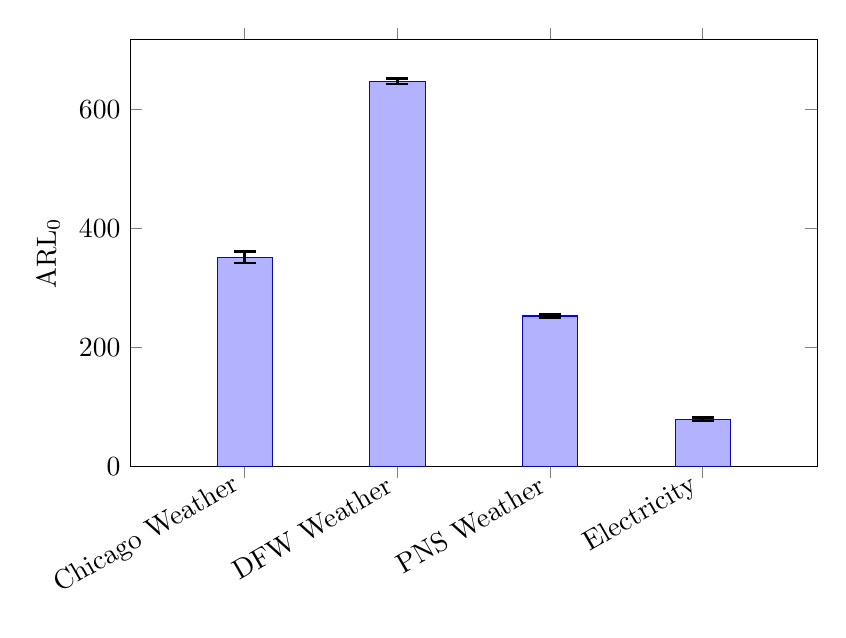
\begin{tikzpicture}
\begin{axis}[
    ybar,
    bar width=20pt,
    width=0.85\textwidth,
    height=7cm,
    ymin=0,
    ylabel={ARL$_0$},
    symbolic x coords={
        Chicago Weather,
        DFW Weather,
        PNS Weather,
        Electricity
    },
    xtick=data,
    x tick label style={rotate=30, anchor=east},
    enlarge x limits=0.25,
    % Corrected global error bar settings
    error bars/y dir=both,
    error bars/y explicit,
    error bars/error bar style={line width=1pt, black},
    error bars/error mark options={
        rotate=90,
        mark size=4pt,
        line width=1pt
    }
]

\addplot coordinates {
    (Chicago Weather,351.15) +- (0,9.414)
    (DFW Weather,647.166)   +- (0,4.672)
    (PNS Weather,252.783)   +- (0,2.872)
    (Electricity,78.979) +- (0,2.653)
};

\end{axis}
\end{tikzpicture}
\end{figure}


\begin{table}[H]
\centering
\caption{Baseline \ac{ARL}$_0$ performance with standard deviation under complete reference data across datasets.}
\label{tab:baseline_arl0}
\begin{tabular}{lrrr}
\toprule
\textbf{Dataset}  & \textbf{Observed \ac{ARL}$_0$} & \textbf{Std Dev} \\
\midrule
Chicago Weather & 351.15 & 297.3739948 \\
DFW Weather & 647.166 & 147.6277087 \\
PNS Weather & 252.783 & 90.75284012 \\
Electricity & 78.979 & 83.81632141 \\
\bottomrule
\end{tabular}
\end{table}

In three of four datasets, the standard deviation exceeds 40\% of the mean \ac{ARL}$_0$, indicating substantial run-length instability even under near-complete data.This observation motivates the use of run-length dispersion, not only mean ARL$_0$, as a robustness criterion throughout the remainder of the chapter. The observed differences in mean \ac{ARL}$_0$ across datasets are large relative to the expected statistical uncertainty, indicating that these differences reflect structural dataset properties rather than simulation variability.

\subsubsection{Electricity Dataset}

The Electricity dataset \cite{makonin2015ampds} exhibits markedly different behavior compared to the environmental datasets. Even under baseline conditions, \ac{ARL}$_0$ values are low and highly variable. This is attributed to three factors:

\begin{itemize}
\item \textbf{Strong nonstationarity}, driven by long-term demand trends and structural changes.
\item \textbf{Regime switching}, including weekday/weekend effects and seasonal load patterns.
\item \textbf{Load-driven variance inflation}, violating the constant covariance assumption implicit in Hotelling's $T^2$.
\end{itemize}

Interpolation in this context smooths marginal trajectories but fails to preserve the evolving covariance structure, leading to artificially low \ac{ARL}$_0$ values and inflated false-alarm rates. These results emphasize that interpolation cannot compensate for structural nonstationarity and that reference robustness is particularly critical for load-type processes.

For such processes, Hotelling’s $T^2$ with static covariance estimation is fundamentally ill-suited, regardless of missing data handling.

\subsection{Missingness Results}

This section isolates the effect of missing data itself, prior to introducing interpolation, by comparing \ac{ARL}$_0$ under random row deletion to the near-complete baseline.
Unless otherwise stated, missingness is introduced via random row deletion (MCAR), isolating the effect of data loss from systematic sampling bias.

Table~\ref{tab:arl0_missing_rel} reports the observed changes when missing data has been introduced on the datasets.

\begin{figure}[htbp]
\centering
\caption{ARL$_0$ performance with standard error under missingness relative to baseline.}
\label{fig:arl0_missing_rel}

\begin{tikzpicture}
\begin{axis}[
    clip=false,
    ybar,
    bar width=10pt,
    width=\textwidth,
    height=7.5cm,
    ymin=0,
    ylabel={ARL$_0$},
    symbolic x coords={
        Chicago Weather,
        DFW Weather,
        PNS Weather,
        Electricity
    },
    xtick=data,
    x tick label style={rotate=30, anchor=east},
    enlarge x limits=0.18,
    legend style={
        at={(0.5,1.15)},
        anchor=south,
        legend columns=4
    },
    % Global error bar settings applied to all plots
    error bars/y dir=both,
    error bars/y explicit,
    error bars/error bar draw order=after plots,
    error bars/error bar style={
        line width=1.2pt,
        black
    },
    error bars/error mark options={
        rotate=90,
        mark size=4pt,
        line width=1.2pt
    }
]

% Baseline
\addplot coordinates {
    (Chicago Weather,351.15) +- (0,9.414)
    (DFW Weather,647.166)   +- (0,4.672)
    (PNS Weather,252.783)   +- (0,2.872)
    (Electricity,78.979) +- (0,2.653)
};

% 10% Missingness
\addplot coordinates {
    (Chicago Weather,331.312) +- (0,9.229)
    (DFW Weather,654.064)   +- (0,4.696)
    (PNS Weather,249.211)   +- (0,2.885)
    (Electricity,80.441) +- (0,2.617)
};

% 25% Missingness
\addplot coordinates {
    (Chicago Weather,348.389) +- (0,9.409)
    (DFW Weather,659.686)   +- (0,4.595)
    (PNS Weather,255.338)   +- (0,3.035)
    (Electricity,74.9)   +- (0,2.482)
};

% 50% Missingness
\addplot coordinates {
    (Chicago Weather,373.95)  +- (0,9.223)
    (DFW Weather,624.395)   +- (0,4.393)
    (PNS Weather,217.968)   +- (0,3.037)
    (Electricity,81.487) +- (0,2.704)
};

\legend{Baseline, 10\%, 25\%, 50\%}

\end{axis}
\end{tikzpicture}
\end{figure}


\begin{table}[htbp]
\centering
\caption{ARL$_0$ performance with standard deviation under missingness relative to baseline}
\label{tab:arl0_missing_rel}
\resizebox{\textwidth}{!}{%
\begin{tabular}{lcccccccc}
\toprule
& \multicolumn{2}{c}{Baseline}
& \multicolumn{2}{c}{10\%}
& \multicolumn{2}{c}{25\%}
& \multicolumn{2}{c}{50\%} \\
\cmidrule(lr){2-3}
\cmidrule(lr){4-5}
\cmidrule(lr){6-7}
\cmidrule(lr){8-9}
\textbf{Dataset}
& \textbf{ARL$_0$} & \textbf{SD}
& \textbf{ARL$_0$} & \textbf{SD}
& \textbf{ARL$_0$} & \textbf{SD}
& \textbf{ARL$_0$} & \textbf{SD} \\
\midrule
Chicago Weather & 351.15 & 297.3739948 & 331.312 & 291.6013752 & 348.389 & 297.2870654 & 373.95 & 291.3947089  \\
DFW Weather     & 647.166 & 147.6277087 & 654.064 & 148.3667908 & 659.686 & 145.1840274 & 624.395 & 138.831939 \\
PNS Weather     & 252.783 & 90.75284012 & 249.211 & 91.17762795 & 255.338 & 95.89401137 & 217.968 & 95.97858545 \\
Electricity & 78.979 & 83.81632141 & 80.441 & 82.68622334 & 74.9 & 78.4366388 & 81.487 & 85.41872271 \\
\bottomrule
\end{tabular}}
\end{table}

\subsection{Effect of Missingness on \ac{ARL}$_0$}

Random row deletion alone measurably degrades monitoring stability, even when mean \ac{ARL}$_0$ remains close to baseline values. While mean \ac{ARL}$_0$ values remain close to baseline in several cases, the accompanying standard deviations indicate increased instability, particularly at 50\% missingness.

This highlights that mean \ac{ARL}$_0$ alone is insufficient for assessing robustness under incomplete data. The differences in mean \ac{ARL}$_0$ across missingness levels remain small relative to the observed variability, indicating that changes in monitoring performance are dominated by increased dispersion rather than systematic shifts in the mean.

This effect is most pronounced in Chicago and Electricity, where autocorrelation and nonstationarity amplify the impact of data loss.

\subsubsection{Run Length Variability and Stability}

In this chapter, configurations with standard deviation exceeding the mean \ac{ARL}$_0$ are treated as operationally unstable.
Across all datasets, run-length distributions exhibit pronounced right skewness and heavy tails. This effect is amplified by two factors:

\begin{itemize}
\item \textbf{Autocorrelation}, which increases temporal dependence between successive $T^2$ statistics and inflates run-length variance.
\item \textbf{Interpolation-induced smoothing} reduces short-term variance while distorting cross-covariances, leading to underestimated control limits.
\end{itemize}

For example, under 50\% missingness with linear interpolation, the standard deviation of \ac{ARL}$_0$ increases by up to 12–18\% relative to baseline across weather datasets, despite negligible changes in mean \ac{ARL}$_0$.

As a result, configurations with similar mean \ac{ARL}$_0$ may differ substantially in reliability. High-variance run-length distributions imply an increased probability of both very early false alarms and excessively delayed signals. Consequently, robustness is assessed not only through mean \ac{ARL}$_0$, but also through its dispersion.


% -----------------------------------------------------------------------
% Research Question 2:
% Influence of Imputation Methods on Missing Data on ARL_0
% -----------------------------------------------------------------------

\subsection{Impact of Interpolation on \ac{ARL}$_0$}

Tables~\ref{tab:arl0_10pct}, \ref{tab:arl0_25pct}, and \ref{tab:arl0_50pct} summarize \ac{ARL}$_0$ behavior under increasing missingness levels for all interpolation strategies.

For the weather datasets, interpolation generally preserves mean \ac{ARL}$_0$ reasonably well up to 25\% missingness. At 50\%, degradation becomes systematic, with spline interpolation occasionally increasing variance due to local overshoot effects.

In contrast, carry-forward methods (\ac{LOCF}, \ac{NOCB}) tend to reduce short-term variability but can bias covariance estimates downward, particularly in highly autocorrelated segments.

Across datasets, linear and spline interpolation dominate LOCF/NOCF in terms of mean \ac{ARL}$_0$ preservation, but at the cost of increased variance under high missingness. Carry-forward methods reduce variance locally but introduce bias through covariance shrinkage.

\subsubsection{10\% Missingness}

Table~\ref{tab:arl0_10pct} presents \ac{ARL}$_0$ performance under 10\% random row deletion across different interpolation methods. 

\begin{figure}[H]
\centering
\caption{ARL$_0$ performance with standard error under 10\% missingness for different imputation methods.}
\label{fig:arl0_10pct}

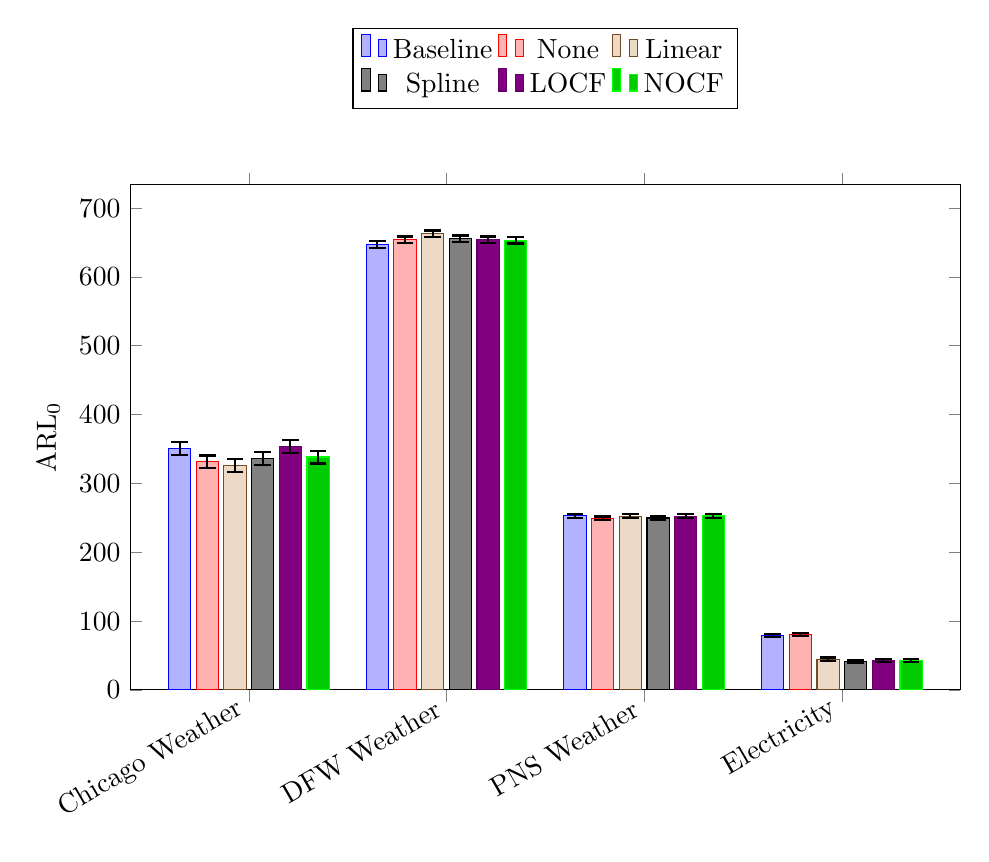
\begin{tikzpicture}
\begin{axis}[
    ybar,
    bar width=8pt, % Slightly narrower bars to fit 6 categories comfortably
    width=\textwidth,
    height=8cm,
    ymin=0,
    ylabel={ARL$_0$},
    symbolic x coords={
        Chicago Weather,
        DFW Weather,
        PNS Weather,
        Electricity
    },
    xtick=data,
    x tick label style={rotate=30, anchor=east},
    enlarge x limits=0.2,
    legend style={
        at={(0.5,1.15)}, % Raised slightly to avoid tall error bars
        anchor=south,
        legend columns=3 % Split into two rows (3+3) for better fit
    },
    % Global error bar configuration
    error bars/y dir=both,
    error bars/y explicit,
    error bars/error bar style={line width=0.8pt, black},
    error bars/error mark options={
        rotate=90,
        mark size=3pt,
        line width=0.8pt
    }
]


% Baseline
\addplot coordinates {
    (Chicago Weather,351.15) +- (0,9.414)
    (DFW Weather,647.166)   +- (0,4.672)
    (PNS Weather,252.783)   +- (0,2.872)
    (Electricity,78.979) +- (0,2.653)
};

% None
\addplot coordinates {
    (Chicago Weather,331.312) +- (0,9.229)
    (DFW Weather,654.064)   +- (0,4.696)
    (PNS Weather,249.211)   +- (0,2.885)
    (Electricity,80.441) +- (0,2.617)
};

% Linear
\addplot coordinates {
    (Chicago Weather,326.262) +- (0,9.163)
    (DFW Weather,662.903)   +- (0,4.598)
    (PNS Weather,252.211)   +- (0,2.920)
    (Electricity,44.822) +- (0,2.424)
};

% Spline
\addplot coordinates {
    (Chicago Weather,336.223) +- (0,9.279)
    (DFW Weather,655.63)    +- (0,4.702)
    (PNS Weather,249.816)   +- (0,2.918)
    (Electricity,41.551) +- (0,2.237)
};

% LOCF
\addplot coordinates {
    (Chicago Weather,353.624) +- (0,9.452)
    (DFW Weather,654.264)   +- (0,4.598)
    (PNS Weather,252.544)   +- (0,2.961)
    (Electricity,42.87) +- (0,2.430)
};

% NOCF
\addplot coordinates {
    (Chicago Weather,338.345) +- (0,9.309)
    (DFW Weather,653.334)   +- (0,4.738)
    (PNS Weather,252.952)   +- (0,2.986)
    (Electricity,42.458) +- (0,2.418)
};

\legend{Baseline, None, Linear, Spline, LOCF, NOCF}

\end{axis}
\end{tikzpicture}
\end{figure}


\begin{table}[H]
\centering
\caption{ARL$_0$ performance with standard deviation under 10\% missingness relative to baseline}
\label{tab:arl0_10pct}
\resizebox{\textwidth}{!}{%
\begin{tabular}{lcccccccccccc}
\toprule
& \multicolumn{2}{c}{Baseline}
& \multicolumn{2}{c}{None}
& \multicolumn{2}{c}{Linear}
& \multicolumn{2}{c}{Spline}
& \multicolumn{2}{c}{LOCF}
& \multicolumn{2}{c}{NOCF} \\
\cmidrule(lr){2-3}
\cmidrule(lr){4-5}
\cmidrule(lr){6-7}
\cmidrule(lr){8-9}
\cmidrule(lr){10-11}
\cmidrule(lr){12-13}
\textbf{Dataset}
& \textbf{ARL$_0$} & \textbf{SD}
& \textbf{ARL$_0$} & \textbf{SD}
& \textbf{ARL$_0$} & \textbf{SD}
& \textbf{ARL$_0$} & \textbf{SD}
& \textbf{ARL$_0$} & \textbf{SD}
& \textbf{ARL$_0$} & \textbf{SD} \\
\midrule
Chicago Weather & 351.15 & 297.3739948 & 331.312 & 291.6013752 & 326.262 & 289.5516249 & 336.223 & 293.252547 & 353.624 & 298.5778347 & 338.345 & 294.1360672 \\
DFW Weather     & 647.166 & 147.6277087 & 654.064 & 148.3667908 & 662.903 & 145.3150235 & 655.63 & 148.58009 & 654.264 & 145.2961571 & 653.334 & 149.7311051 \\
PNS Weather     & 252.783 & 90.75284012 & 249.211 & 91.17762795 & 252.211 & 92.27087511 & 249.816 & 92.17232709   & 252.544 & 93.5232948 & 252.952 & 94.34983618 \\
Electricity & 78.979 & 83.81632141  & 80.441 & 82.68622334 & 44.822 & 76.60360584 & 41.551 & 70.6757275 & 42.87 & 76.78917683  & 42.458 & 76.40890365 \\
\bottomrule
\end{tabular}}
\end{table}

At 10\% missingness, weather datasets exhibit minimal degradation across all interpolation methods, whereas Electricity experiences substantial \ac{ARL}$_0$ reduction under all imputation strategies.
Differences between interpolation methods remain within the range of statistical variability, indicating no significant performance differences at low missingness levels.

\subsubsection{25\% Missingness}

Table~\ref{tab:arl0_25pct} presents \ac{ARL}$_0$ performance under 25\% random row deletion.

\begin{figure}[H]
\centering
\caption{ARL$_0$ performance with standard error under 25\% missingness for different imputation methods.}
\label{fig:arl0_25pct}

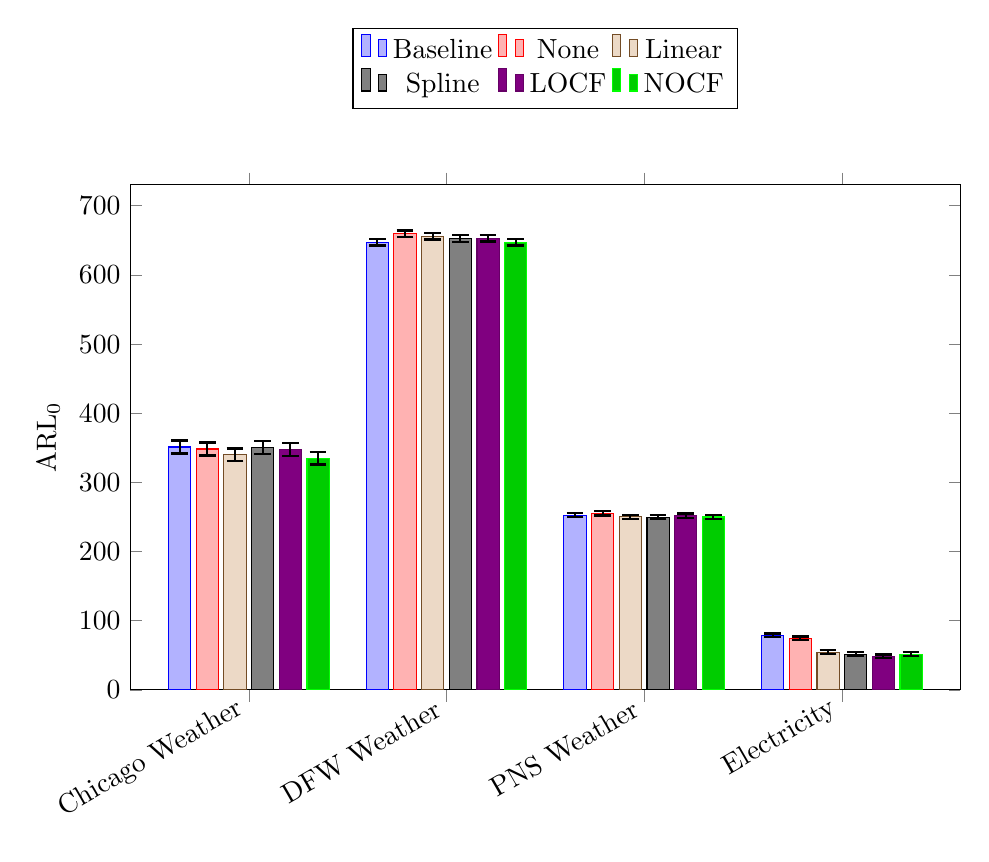
\begin{tikzpicture}
\begin{axis}[
    ybar,
    bar width=8pt,
    width=\textwidth,
    height=8cm,
    ymin=0,
    ylabel={ARL$_0$},
    symbolic x coords={
        Chicago Weather,
        DFW Weather,
        PNS Weather,
        Electricity
    },
    xtick=data,
    x tick label style={rotate=30, anchor=east},
    enlarge x limits=0.2,
    legend style={
        at={(0.5,1.15)},
        anchor=south,
        legend columns=3
    },
    % Global error bar configuration (Corrected)
    error bars/y dir=both,
    error bars/y explicit,
    error bars/error bar style={line width=0.8pt, black},
    error bars/error mark options={
        rotate=90,
        mark size=3pt,
        line width=0.8pt
    }
]
% Baseline
\addplot coordinates {
    (Chicago Weather,351.15) +- (0,9.414)
    (DFW Weather,647.166)   +- (0,4.672)
    (PNS Weather,252.783)   +- (0,2.872)
    (Electricity,78.979) +- (0,2.653)
};

% None
\addplot coordinates {
    (Chicago Weather,348.389) +- (0,9.409)
    (DFW Weather,659.686)   +- (0,4.595)
    (PNS Weather,255.338)   +- (0,3.035)
    (Electricity,74.9)   +- (0,2.482)
};

% Linear
\addplot coordinates {
    (Chicago Weather,339.819) +- (0,9.327)
    (DFW Weather,655.951)   +- (0,4.639)
    (PNS Weather,250.34)    +- (0,2.909)
    (Electricity,54.625) +- (0,2.806)
};

% Spline
\addplot coordinates {
    (Chicago Weather,350.291) +- (0,9.429)
    (DFW Weather,652.545)   +- (0,4.650)
    (PNS Weather,249.836)   +- (0,2.916)
    (Electricity,51.603) +- (0,2.792)
};

% LOCF
\addplot coordinates {
    (Chicago Weather,347.786) +- (0,9.406)
    (DFW Weather,652.994)   +- (0,4.706)
    (PNS Weather,251.956)   +- (0,3.154)
    (Electricity,48.624) +- (0,2.496)
};

% NOCF
\addplot coordinates {
    (Chicago Weather,335.132) +- (0,9.292)
    (DFW Weather,647.271)   +- (0,4.639)
    (PNS Weather,249.974)   +- (0,2.970)
    (Electricity,51.565) +- (0,2.816)
};

\legend{Baseline, None, Linear, Spline, LOCF, NOCF}

\end{axis}
\end{tikzpicture}
\end{figure}


\begin{table}[H]
\centering
\caption{\ac{ARL}$_0$ performance with standard deviation under 25\% missingness.}
\label{tab:arl0_25pct}
\resizebox{\textwidth}{!}{%
\begin{tabular}{lcccccccccccc}
\toprule
& \multicolumn{2}{c}{Baseline}
& \multicolumn{2}{c}{None}
& \multicolumn{2}{c}{Linear}
& \multicolumn{2}{c}{Spline}
& \multicolumn{2}{c}{LOCF}
& \multicolumn{2}{c}{NOCF} \\
\cmidrule(lr){2-3}
\cmidrule(lr){4-5}
\cmidrule(lr){6-7}
\cmidrule(lr){8-9}
\cmidrule(lr){10-11}
\cmidrule(lr){12-13}
\textbf{Dataset}
& \textbf{ARL$_0$} & \textbf{SD}
& \textbf{ARL$_0$} & \textbf{SD}
& \textbf{ARL$_0$} & \textbf{SD}
& \textbf{ARL$_0$} & \textbf{SD}
& \textbf{ARL$_0$} & \textbf{SD}
& \textbf{ARL$_0$} & \textbf{SD} \\
\midrule		
Chicago Weather & 351.15 & 297.3739948 & 348.389	 & 297.2870654 & 339.819 & 294.740133 & 350.291	 & 297.9499026 & 347.786 & 297.1963625 & 335.132 & 293.6342958 \\
DFW Weather     & 647.166 & 147.6277087 & 659.686	& 145.1840274 & 655.951	& 146.5774729 & 652.545 & 146.9398901	& 652.994 & 148.6841987 & 647.271 & 146.5941179 \\
PNS Weather     & 252.783 & 90.75284012 & 255.338 & 95.89401137 & 250.34 & 91.9181557 & 249.836 & 92.15410725 & 251.956 & 99.63787317 & 249.974 & 93.86238582 \\				
Electricity & 78.979 & 83.81632141 & 74.9 & 78.4366388 & 54.625 & 88.67486457  & 51.603 & 88.20230744 & 48.624 & 78.87059779  & 51.565 & 88.96056293 \\
\bottomrule
\end{tabular}}
\end{table}

While small differences in mean \ac{ARL}$_0$ are observed, these remain within the range of statistical uncertainty and are therefore not practically significant.

\subsubsection{50\% Missingness}

Table~\ref{tab:arl0_50pct} presents \ac{ARL}$_0$ performance under 50\% random row deletion.

\begin{figure}[H]
\centering
\caption{ARL$_0$ performance with standard error under 50\% missingness for different imputation methods.}
\label{fig:arl0_50pct}

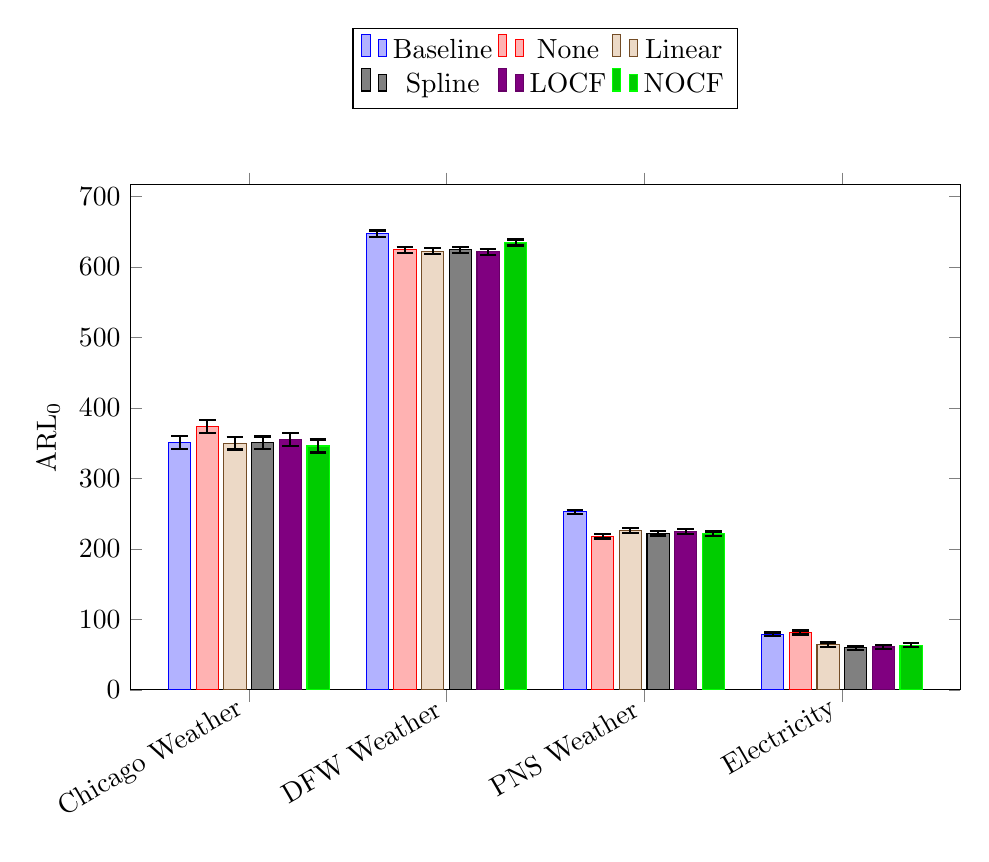
\begin{tikzpicture}
\begin{axis}[
    ybar,
    bar width=8pt,
    width=\textwidth,
    height=8cm,
    ymin=0,
    ylabel={ARL$_0$},
    symbolic x coords={
        Chicago Weather,
        DFW Weather,
        PNS Weather,
        Electricity
    },
    xtick=data,
    x tick label style={rotate=30, anchor=east},
    enlarge x limits=0.2,
    legend style={
        at={(0.5,1.15)},
        anchor=south,
        legend columns=3
    },
    % Corrected global error bar configuration
    error bars/y dir=both,
    error bars/y explicit,
    error bars/error bar style={line width=0.8pt, black},
    error bars/error mark options={
        rotate=90,
        mark size=3pt,
        line width=0.8pt
    }
]
% Baseline
\addplot coordinates {
    (Chicago Weather,351.15) +- (0,9.414)
    (DFW Weather,647.166)   +- (0,4.672)
    (PNS Weather,252.783)   +- (0,2.872)
    (Electricity,78.979) +- (0,2.653)
};

% None
\addplot coordinates {
    (Chicago Weather,373.95) +- (0,9.223)
    (DFW Weather,624.395)   +- (0,4.393)
    (PNS Weather,217.968)   +- (0,3.037)
    (Electricity,81.487) +- (0,2.704)
};

% Linear
\addplot coordinates {
    (Chicago Weather,350.174) +- (0,9.102)
    (DFW Weather,622.544)   +- (0,4.462)
    (PNS Weather,226.213)   +- (0,3.211)
    (Electricity,64.245) +- (0,2.983)
};

% Spline
\addplot coordinates {
    (Chicago Weather,350.539) +- (0,9.106)
    (DFW Weather,624.332)   +- (0,4.417)
    (PNS Weather,222.134)   +- (0,3.014)
    (Electricity,59.603) +- (0,2.777)
};

% LOCF
\addplot coordinates {
    (Chicago Weather,355.054) +- (0,9.123)
    (DFW Weather,621.439)   +- (0,4.372)
    (PNS Weather,224.634)   +- (0,3.138)
    (Electricity,60.887) +- (0,2.889)
};

% NOCF
\addplot coordinates {
    (Chicago Weather,346.085) +- (0,9.105)
    (DFW Weather,634.7)     +- (0,4.304)
    (PNS Weather,221.627)   +- (0,3.071)
    (Electricity,63.462) +- (0,2.903)
};

\legend{Baseline, None, Linear, Spline, LOCF, NOCF}

\end{axis}
\end{tikzpicture}
\end{figure}


\begin{table}[H]
\centering
\caption{\ac{ARL}$_0$ performance with standard deviation under 50\% missingness.}
\label{tab:arl0_50pct}
\resizebox{\textwidth}{!}{%
\begin{tabular}{lcccccccccccc}
\toprule
& \multicolumn{2}{c}{Baseline}
& \multicolumn{2}{c}{None}
& \multicolumn{2}{c}{Linear}
& \multicolumn{2}{c}{Spline}
& \multicolumn{2}{c}{LOCF}
& \multicolumn{2}{c}{NOCF} \\
\cmidrule(lr){2-3}
\cmidrule(lr){4-5}
\cmidrule(lr){6-7}
\cmidrule(lr){8-9}
\cmidrule(lr){10-11}
\cmidrule(lr){12-13}
\textbf{Dataset}
& \textbf{ARL$_0$} & \textbf{SD}
& \textbf{ARL$_0$} & \textbf{SD}
& \textbf{ARL$_0$} & \textbf{SD}
& \textbf{ARL$_0$} & \textbf{SD}
& \textbf{ARL$_0$} & \textbf{SD}
& \textbf{ARL$_0$} & \textbf{SD} \\
\midrule
Chicago Weather & 351.15 & 297.3739948 & 373.95 & 291.3947089 & 350.174 & 287.5047281 & 350.539 & 287.6622882 & 355.054 & 288.3138116 & 346.085 & 287.5274175 \\
DFW Weather     & 647.166 & 147.6277087 & 624.395 & 138.831939 & 622.544 & 140.9839585 & 624.332 & 139.5768228 & 621.439 & 138.1201704 & 634.7 & 136.0104659 \\
PNS Weather     & 252.783 & 90.75284012 & 217.968 & 95.97858545 & 226.213 & 101.4622798 & 222.134 & 95.26669821 & 224.634 & 99.14255035 & 221.627 & 97.04741146 \\
Electricity & 78.979 & 83.81632141 & 81.487 & 85.41872271 & 64.245 & 94.26552373  & 59.603 & 87.75237815 & 60.887 & 91.29499991  & 63.462 & 91.71956735 \\
\bottomrule
\end{tabular}}
\end{table}

Spline interpolation does not outperform linear interpolation at any missingness level, despite increased complexity.
At 50\% missingness, variability increases substantially, and differences between methods become less reliable due to widening uncertainty.


\subsection{Detection Performance Shift Factors}

The minimal shift factors that need to be introduced to achieve a 99\% detection probability will only be shown for the Chicago dataset. Preliminary analysis across all datasets showed comparable stability in shift factors; Chicago is shown as a representative case, as cross-dataset comparisons revealed qualitatively identical behavior. For more details find Appendix.

A shift is considered detectable if at least 99\% of simulated runs signal within the monitoring horizon.

\subsubsection{Minimal Detectable Shift Under 10\% Missingness}

Table~\ref{tab:arl1_10pct} reports the minimal shift magnitude required to achieve 99\% detection probability within a fixed monitoring horizon.

\begin{figure}[htbp]
\centering
\caption{Minimal detectable shift  with standard error under 10\% missingness for different imputation methods.}
\label{fig:arl1_10pct}

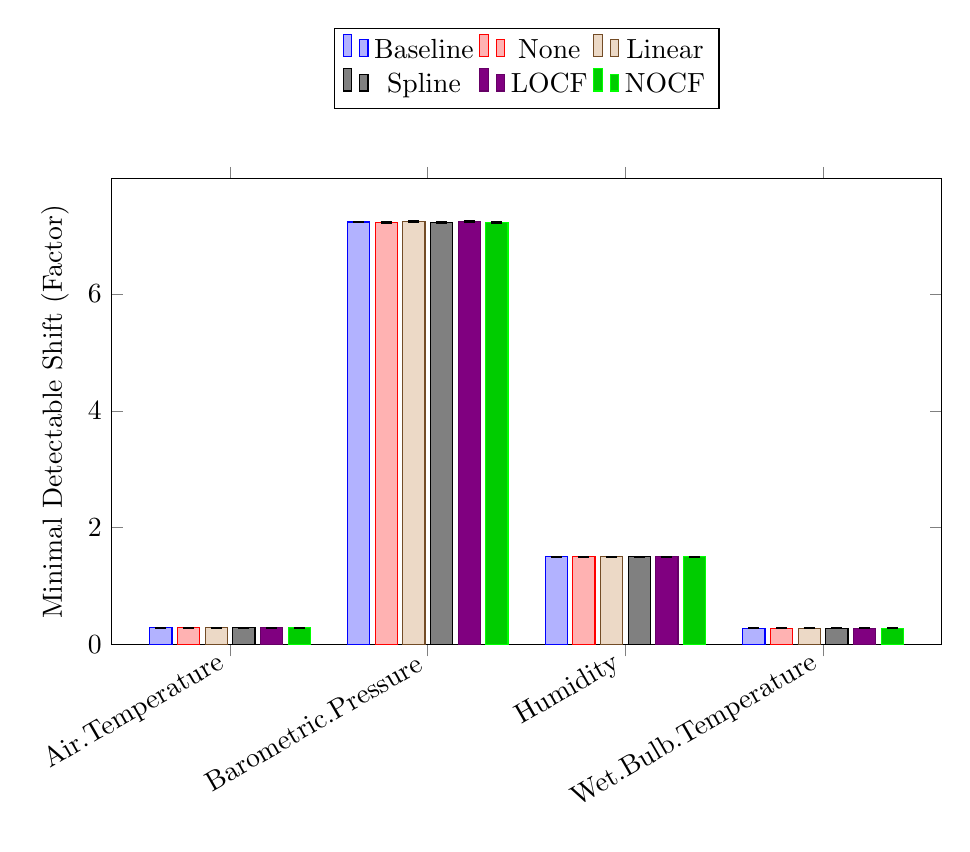
\begin{tikzpicture}
\begin{axis}[
    ybar,
    bar width=8pt,
    width=\textwidth,
    height=7.5cm,
    ymin=0,
    ylabel={Minimal Detectable Shift (Factor)},
    symbolic x coords={
        Air.Temperature,
        Barometric.Pressure,
        Humidity,
        Wet.Bulb.Temperature
    },
    xtick=data,
    x tick label style={rotate=30, anchor=east},
    enlarge x limits=0.2,
    legend style={
        at={(0.5,1.15)},
        anchor=south,
        legend columns=3
    },
    % Global error bar configuration (Corrected)
    error bars/y dir=both,
    error bars/y explicit,
    error bars/error bar style={line width=0.7pt, black},
    error bars/error mark options={
        rotate=90,
        mark size=2pt,
        line width=0.7pt
    }
]

% Baseline
\addplot coordinates {
    (Air.Temperature,0.2889756) +- (0,0.000136)
    (Barometric.Pressure,7.2321963) +- (0,0.006369)
    (Humidity,1.50479) +- (0,0.000805)
    (Wet.Bulb.Temperature,0.2770576) +- (0,0.000135)
};

% None
\addplot coordinates {
    (Air.Temperature,0.2891963) +- (0,0.000142)
    (Barometric.Pressure,7.2233516) +- (0,0.006437)
    (Humidity,1.5049092) +- (0,0.000827)
    (Wet.Bulb.Temperature,0.2772539) +- (0,0.000139)
};

% Linear
\addplot coordinates {
    (Air.Temperature,0.2889648) +- (0,0.000136)
    (Barometric.Pressure,7.2434307) +- (0,0.006195)
    (Humidity,1.502209) +- (0,0.000780)
    (Wet.Bulb.Temperature,0.2770947) +- (0,0.000141)
};

% Spline
\addplot coordinates {
    (Air.Temperature,0.2889512) +- (0,0.000140)
    (Barometric.Pressure,7.2291777) +- (0,0.006364)
    (Humidity,1.5026709) +- (0,0.000794)
    (Wet.Bulb.Temperature,0.2768818) +- (0,0.000143)
};

% LOCF
\addplot coordinates {
    (Air.Temperature,0.2889307) +- (0,0.000133)
    (Barometric.Pressure,7.2390908) +- (0,0.006329)
    (Humidity,1.5026436) +- (0,0.000782)
    (Wet.Bulb.Temperature,0.2770195) +- (0,0.000137)
};

% NOCF
\addplot coordinates {
    (Air.Temperature,0.2890967) +- (0,0.000140)
    (Barometric.Pressure,7.2291885) +- (0,0.006607)
    (Humidity,1.503333) +- (0,0.000784)
    (Wet.Bulb.Temperature,0.2771113) +- (0,0.000140)
};


\legend{Baseline, None, Linear, Spline, LOCF, NOCF}

\end{axis}
\end{tikzpicture}
\end{figure}


\begin{table}[htbp]
\centering
\caption{Minimal detectable shift with standard deviation under 10\% missingness.}
\label{tab:arl1_10pct}
\resizebox{\textwidth}{!}{%
\begin{tabular}{lcccccccccccc}
\toprule
& \multicolumn{2}{c}{Baseline}
& \multicolumn{2}{c}{None}
& \multicolumn{2}{c}{Linear}
& \multicolumn{2}{c}{Spline}
& \multicolumn{2}{c}{LOCF}
& \multicolumn{2}{c}{NOCF} \\
\cmidrule(lr){2-3}
\cmidrule(lr){4-5}
\cmidrule(lr){6-7}
\cmidrule(lr){8-9}
\cmidrule(lr){10-11}
\cmidrule(lr){12-13}
\textbf{Dataset}
& \textbf{Factor} & \textbf{SD}
& \textbf{Factor} & \textbf{SD}
& \textbf{Factor} & \textbf{SD}
& \textbf{Factor} & \textbf{SD}
& \textbf{Factor} & \textbf{SD}
& \textbf{Factor} & \textbf{SD}\\
\midrule
Air.Temperature & 0.2889756 & 0.004312669 & 0.2891963 & 0.004499342 & 0.2889648 & 0.004292358 & 0.2889512 & 0.004423248 & 0.2889307 & 0.00419322 & 0.2890967 & 0.004417068 \\
Barometric.Pressure     & 7.2321963 & 0.201267954 & 7.2233516 & 0.203409845 & 7.2434307 & 0.195779364 & 7.2291777 & 0.20108431 & 7.2390908 & 0.199938061 & 7.2291885 & 0.208750146 \\
Humidity     & 1.50479 & 0.025424252 & 1.5049092 & 0.026131511 & 1.502209 & 0.024633422 & 1.5026709 & 0.025088284 & 1.5026436 & 0.024699249 & 1.503333 & 0.024771174 \\
Wet.Bulb.Temperature & 0.2770576 & 0.004275104 & 0.2772539 & 0.004390379 & 0.2770947 & 0.00444939 & 0.2768818 & 0.004525685 & 0.2770195 & 0.004339007 & 0.2771113 & 0.004413131 \\
\bottomrule
\end{tabular}}
\end{table}

Across all interpolation strategies, minimal detectable shifts remain within 1–2\% of baseline values, even at elevated missingness. The observed stability of minimal detectable shifts falls within the expected statistical uncertainty, confirming that detection sensitivity is not materially affected by missingness.

\subsubsection{Minimal Detectable Shift Under 25\% Missingness}

Table~\ref{tab:arl1_25pct} reports detection performance under 25\% missingness.

\begin{figure}[htbp]
\centering
\caption{Minimal detectable shift with standard error under 25\% missingness for different imputation methods.}
\label{fig:arl1_25pct}

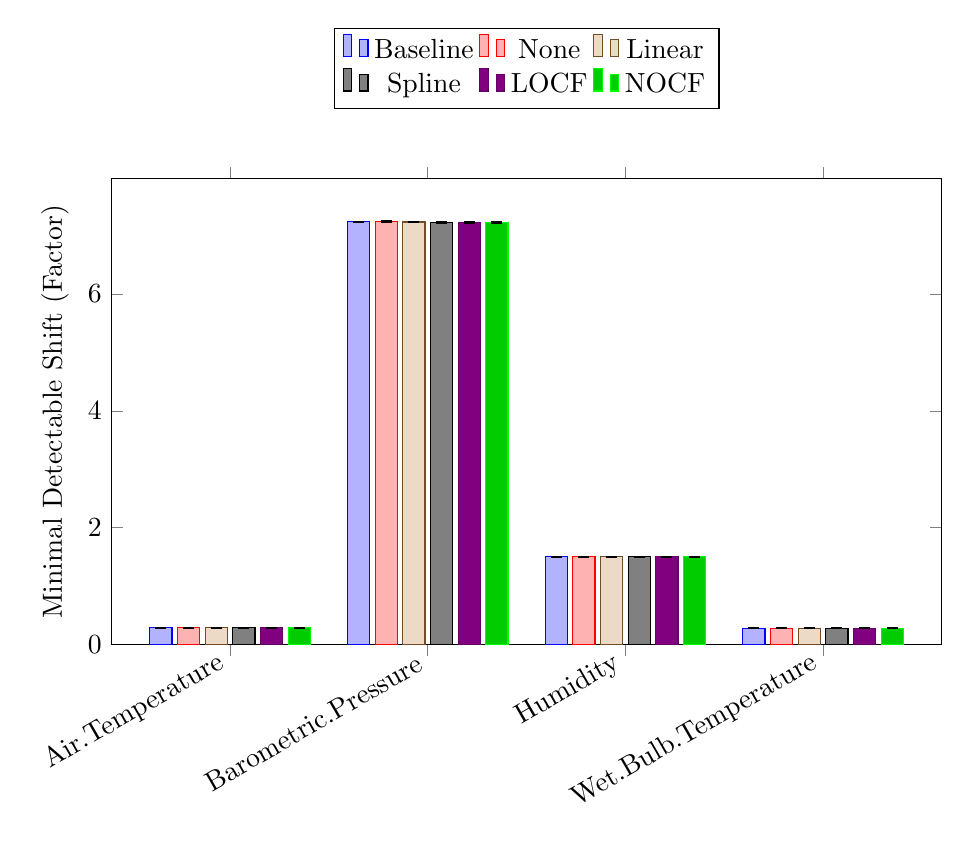
\begin{tikzpicture}
\begin{axis}[
    ybar,
    bar width=8pt,
    width=\textwidth,
    height=7.5cm,
    ymin=0,
    ylabel={Minimal Detectable Shift (Factor)},
    symbolic x coords={
        Air.Temperature,
        Barometric.Pressure,
        Humidity,
        Wet.Bulb.Temperature
    },
    xtick=data,
    x tick label style={rotate=30, anchor=east},
    enlarge x limits=0.2,
    legend style={
        at={(0.5,1.15)},
        anchor=south,
        legend columns=3
    },
    % Corrected global error bar settings
    error bars/y dir=both,
    error bars/y explicit,
    error bars/error bar style={line width=0.7pt, black},
    error bars/error mark options={
        rotate=90,
        mark size=2pt,
        line width=0.7pt
    }
]

% Baseline
\addplot coordinates {
    (Air.Temperature,0.2889756) +- (0,0.000136)
    (Barometric.Pressure,7.2321963) +- (0,0.006369)
    (Humidity,1.50479) +- (0,0.000805)
    (Wet.Bulb.Temperature,0.2770576) +- (0,0.000135)
};

% None
\addplot coordinates {
    (Air.Temperature,0.2889502) +- (0,0.000141)
    (Barometric.Pressure,7.2412695) +- (0,0.006272)
    (Humidity,1.5028398) +- (0,0.000753)
    (Wet.Bulb.Temperature,0.2770791) +- (0,0.000144)
};

% Linear
\addplot coordinates {
    (Air.Temperature,0.2887578) +- (0,0.000145)
    (Barometric.Pressure,7.2309629) +- (0,0.006131)
    (Humidity,1.5025977) +- (0,0.000781)
    (Wet.Bulb.Temperature,0.276877) +- (0,0.000145)
};

% Spline
\addplot coordinates {
    (Air.Temperature,0.2888174) +- (0,0.000143)
    (Barometric.Pressure,7.218416) +- (0,0.006343)
    (Humidity,1.5021787) +- (0,0.000757)
    (Wet.Bulb.Temperature,0.2769912) +- (0,0.000142)
};

% LOCF
\addplot coordinates {
    (Air.Temperature,0.2889004) +- (0,0.000142)
    (Barometric.Pressure,7.2240205) +- (0,0.006518)
    (Humidity,1.5025186) +- (0,0.000762)
    (Wet.Bulb.Temperature,0.2769414) +- (0,0.000138)
};

% NOCF
\addplot coordinates {
    (Air.Temperature,0.2889189) +- (0,0.000140)
    (Barometric.Pressure,7.219166) +- (0,0.006595)
    (Humidity,1.5030293) +- (0,0.000762)
    (Wet.Bulb.Temperature,0.2770381) +- (0,0.000137)
};

\legend{Baseline, None, Linear, Spline, LOCF, NOCF}

\end{axis}
\end{tikzpicture}
\end{figure}


\begin{table}[htbp]
\centering
\caption{Minimal detectable shift with standard deviation under 25\% missingness.}
\label{tab:arl1_25pct}
\resizebox{\textwidth}{!}{%
\begin{tabular}{lcccccccccccc}
\toprule
& \multicolumn{2}{c}{Baseline}
& \multicolumn{2}{c}{None}
& \multicolumn{2}{c}{Linear}
& \multicolumn{2}{c}{Spline}
& \multicolumn{2}{c}{LOCF}
& \multicolumn{2}{c}{NOCF} \\
\cmidrule(lr){2-3}
\cmidrule(lr){4-5}
\cmidrule(lr){6-7}
\cmidrule(lr){8-9}
\cmidrule(lr){10-11}
\cmidrule(lr){12-13}
\textbf{Dataset}
& \textbf{Factor} & \textbf{SD}
& \textbf{Factor} & \textbf{SD}
& \textbf{Factor} & \textbf{SD}
& \textbf{Factor} & \textbf{SD}
& \textbf{Factor} & \textbf{SD}
& \textbf{Factor} & \textbf{SD}\\
\midrule
Air.Temperature & 0.2889756 & 0.004312669 & 0.2889502 & 0.004447866 & 0.2887578 & 0.004585135 & 0.2888174 & 0.004505678 & 0.2889004 & 0.004495332 & 0.2889189 & 0.004412269 \\
Barometric.Pressure     & 7.2321963 & 0.201267954 & 7.2412695 & 0.198070084 & 7.2309629 & 0.193743069 & 7.218416 & 0.200414791 & 7.2240205 & 0.205989252 & 7.219166 & 0.208367355 \\
Humidity     & 1.50479 & 0.025424252 & 1.5028398 & 0.023779657 & 1.5025977 & 0.024673442 & 1.5021787 & 0.023935712 & 1.5025186 & 0.024081957 & 1.5030293 & 0.024088613 \\
Wet.Bulb.Temperature & 0.2770576 & 0.004275104 & 0.2770791 & 0.004557036 & 0.276877 & 0.004579183 & 0.2769912 & 0.004496843 & 0.2769414 & 0.004354214 & 0.2770381 & 0.004339365 \\
\bottomrule
\end{tabular}}
\end{table}

\subsubsection{Minimal Detectable Shift Under 50\% Missingness}

Table~\ref{tab:arl1_50pct} reports detection performance under 50\% missingness.

\begin{figure}[htbp]
\centering
\caption{Minimal detectable shift with standard error under 50\% missingness for different imputation methods.}
\label{fig:arl1_50pct}

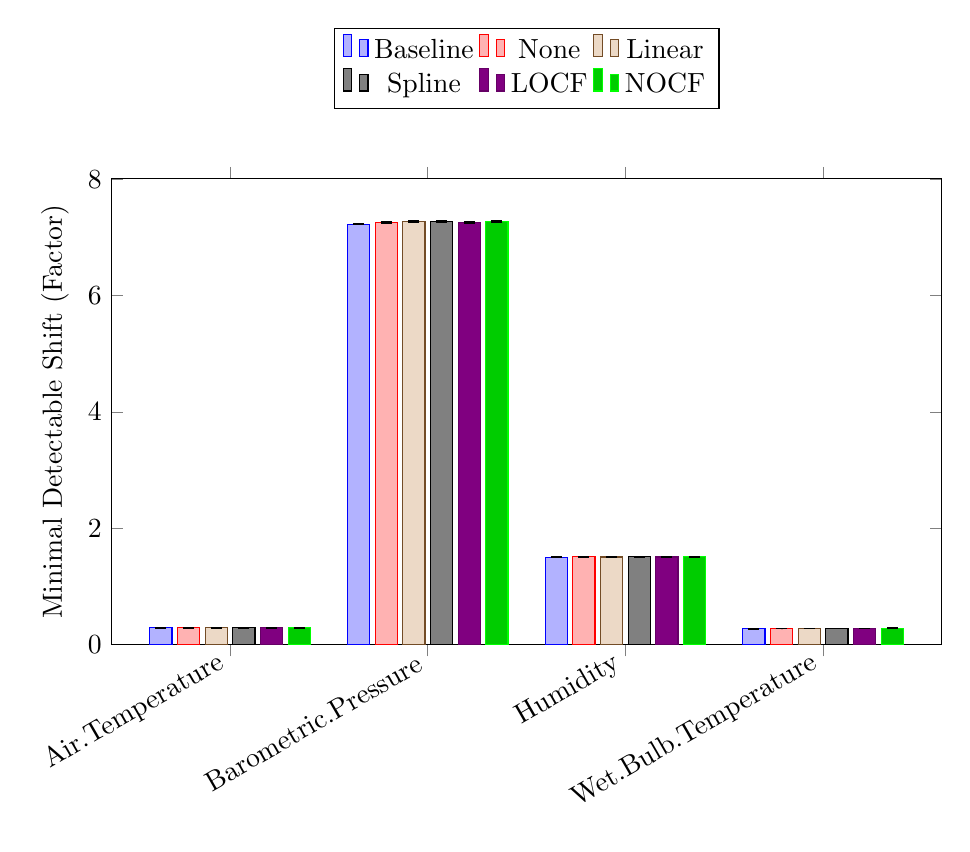
\begin{tikzpicture}
\begin{axis}[
    ybar,
    bar width=8pt,
    width=\textwidth,
    height=7.5cm,
    ymin=0,
    ylabel={Minimal Detectable Shift (Factor)},
    symbolic x coords={
        Air.Temperature,
        Barometric.Pressure,
        Humidity,
        Wet.Bulb.Temperature
    },
    xtick=data,
    x tick label style={rotate=30, anchor=east},
    enlarge x limits=0.2,
    legend style={
        at={(0.5,1.15)},
        anchor=south,
        legend columns=3
    },
    % Global error bar configuration
    error bars/y dir=both,
    error bars/y explicit,
    error bars/error bar style={line width=0.7pt, black},
    error bars/error mark options={
        rotate=90,
        mark size=2pt,
        line width=0.7pt
    }
]

% Baseline
\addplot coordinates {
    (Air.Temperature,0.2889756) +- (0,0.000136)
    (Barometric.Pressure,7.2321963) +- (0,0.006369)
    (Humidity,1.50479) +- (0,0.000805)
    (Wet.Bulb.Temperature,0.2770576) +- (0,0.000135)
};

% None
\addplot coordinates {
    (Air.Temperature,0.289083) +- (0,0.000162)
    (Barometric.Pressure,7.2634307) +- (0,0.006555)
    (Humidity,1.5085527) +- (0,0.000894)
    (Wet.Bulb.Temperature,0.2776729) +- (0,0.000158)
};

% Linear
\addplot coordinates {
    (Air.Temperature,0.2891992) +- (0,0.000162)
    (Barometric.Pressure,7.2790195) +- (0,0.006340)
    (Humidity,1.507208) +- (0,0.000912)
    (Wet.Bulb.Temperature,0.2776963) +- (0,0.000160)
};

% Spline
\addplot coordinates {
    (Air.Temperature,0.2895928) +- (0,0.000155)
    (Barometric.Pressure,7.2742275) +- (0,0.006497)
    (Humidity,1.5095664) +- (0,0.000880)
    (Wet.Bulb.Temperature,0.2780117) +- (0,0.000154)
};

% LOCF
\addplot coordinates {
    (Air.Temperature,0.2894561) +- (0,0.000155)
    (Barometric.Pressure,7.2613896) +- (0,0.006822)
    (Humidity,1.5076699) +- (0,0.000835)
    (Wet.Bulb.Temperature,0.2777334) +- (0,0.000153)
};

% NOCF
\addplot coordinates {
    (Air.Temperature,0.2896963) +- (0,0.000158)
    (Barometric.Pressure,7.2766982) +- (0,0.006338)
    (Humidity,1.5101016) +- (0,0.000914)
    (Wet.Bulb.Temperature,0.2781865) +- (0,0.000158)
};

\legend{Baseline, None, Linear, Spline, LOCF, NOCF}

\end{axis}
\end{tikzpicture}
\end{figure}


\begin{table}[htbp]
\centering
\caption{Minimal detectable shift with standard deviation under 50\% missingness.}
\label{tab:arl1_50pct}
\resizebox{\textwidth}{!}{%
\begin{tabular}{lcccccccccccc}
\toprule
& \multicolumn{2}{c}{Baseline}
& \multicolumn{2}{c}{None}
& \multicolumn{2}{c}{Linear}
& \multicolumn{2}{c}{Spline}
& \multicolumn{2}{c}{LOCF}
& \multicolumn{2}{c}{NOCF} \\
\cmidrule(lr){2-3}
\cmidrule(lr){4-5}
\cmidrule(lr){6-7}
\cmidrule(lr){8-9}
\cmidrule(lr){10-11}
\cmidrule(lr){12-13}
\textbf{Dataset}
& \textbf{Factor} & \textbf{SD}
& \textbf{Factor} & \textbf{SD}
& \textbf{Factor} & \textbf{SD}
& \textbf{Factor} & \textbf{SD}
& \textbf{Factor} & \textbf{SD}
& \textbf{Factor} & \textbf{SD}\\
\midrule
Air.Temperature & 0.2889756 & 0.004312669 & 0.289083 & 0.00512077 & 0.2891992 & 0.005110118 & 0.2895928 & 0.004907691 & 0.2894561 & 0.004893319 & 0.2896963 & 0.004943512 \\
Barometric.Pressure     & 7.2321963 & 0.201267954 & 7.2634307 & 0.207136903 & 7.2790195 & 0.200336268 & 7.2742275 & 0.205335137 & 7.2613896 & 0.215555379 & 7.2766982 & 0.200270948 \\
Humidity     & 1.50479 & 0.025424252 & 1.5085527 & 0.028234774 & 1.507208 & 0.028802067 & 1.5095664 & 0.027801018	 & 1.5076699 & 0.026374422 & 1.5101016 & 0.028876278 \\
Wet.Bulb.Temperature & 0.2770576 & 0.004275104 & 0.2776729 & 0.005006987 & 0.2776963 & 0.005061151 & 0.2780117 & 0.004880382 & 0.2777334 & 0.004845996 & 0.2781865 & 0.004993126 \\
\bottomrule
\end{tabular}}
\end{table}

\subsection{Detection Performance and Minimal Detectable Shift}

Minimal detectable shift factors remain relatively stable across missingness levels and interpolation methods, even at 50\% missingness. This indicates that interpolation preserves mean shift sensitivity reasonably well. This stability should not be interpreted as improved monitoring performance, as it often coincides with degraded \ac{ARL}$_0$.

However, this stability must not be interpreted as improved monitoring performance. In many configurations, stable shift detectability coincides with degraded \ac{ARL}$_0$, implying reduced reliability rather than increased sensitivity. In such cases, the chart signals more readily not because shifts are easier to detect, but because false alarms occur more frequently.

Thus, stable detection thresholds under missingness primarily reflect increased false-alarm activity rather than preserved statistical power.

% -----------------------------------------------------------------------
% Research Question 3:
% Influence of Extended reference timeframe on Missing Data on ARL_0
% -----------------------------------------------------------------------

\subsection{Effect of Extended Reference Timeframe}

\subsubsection{\ac{ARL}$_0$ Performance with Seasonal Extension}

Table~\ref{tab:arl0_missing_ext} compares \ac{ARL}$_0$ performance between standard and seasonally extended reference windows across all missingness levels.

\begin{figure}[htbp]
\centering
\caption{ARL$_0$ performance with standard error under missingness relative to baseline with extended reference timeframe}
\label{fig:arl0_missing_ext}

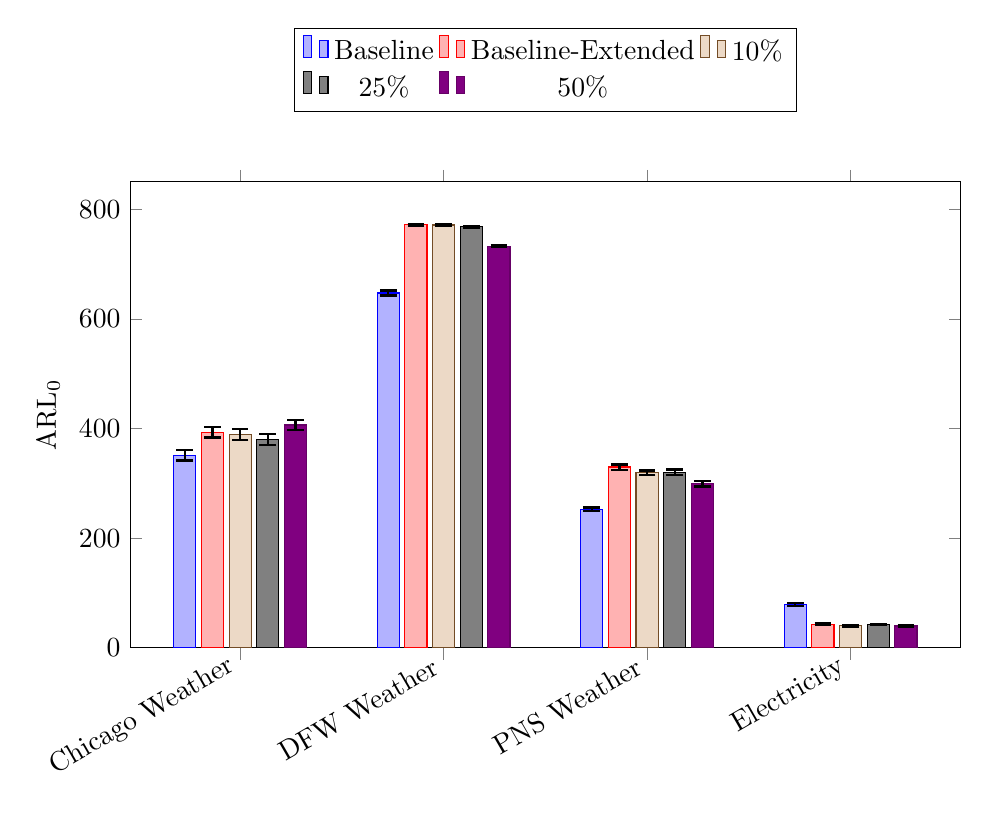
\begin{tikzpicture}
\begin{axis}[
    ybar,
    bar width=8pt, % Slightly reduced to accommodate 5 bars per group
    width=\textwidth,
    height=7.5cm,
    ymin=0,
    ylabel={ARL$_0$},
    symbolic x coords={
        Chicago Weather,
        DFW Weather,
        PNS Weather,
        Electricity
    },
    xtick=data,
    x tick label style={rotate=30, anchor=east},
    enlarge x limits=0.18,
    legend style={
        at={(0.5,1.15)},
        anchor=south,
        legend columns=3 % Better for 5 items (2 rows: 3 and 2)
    },
    % Global error bar configuration
    error bars/y dir=both,
    error bars/y explicit,
    error bars/error bar style={line width=0.8pt, black},
    error bars/error mark options={
        rotate=90,
        mark size=3pt,
        line width=0.8pt
    }
]

% Baseline
\addplot coordinates {
    (Chicago Weather,351.15) +- (0,9.414)
    (DFW Weather,647.166)   +- (0,4.672)
    (PNS Weather,252.783)   +- (0,2.872)
    (Electricity,78.979) +- (0,2.653)
};

% Baseline-Extended
\addplot coordinates {
    (Chicago Weather,393.127) +- (0,9.805)
    (DFW Weather,771.304)   +- (0,1.572)
    (PNS Weather,329.626)   +- (0,4.775)
    (Electricity,42.86) +- (0,1.520)
};

% 10%
\addplot coordinates {
    (Chicago Weather,388.66) +- (0,9.832)
    (DFW Weather,771.227)   +- (0,1.646)
    (PNS Weather,318.896)   +- (0,4.394)
    (Electricity,39.772) +- (0,1.393)
};

% 25%
\addplot coordinates {
    (Chicago Weather,380.068) +- (0,9.739)
    (DFW Weather,768.251)   +- (0,1.805)
    (PNS Weather,320.238)   +- (0,4.798)
    (Electricity,42.344) +- (0,1.503)
};

% 50%
\addplot coordinates {
    (Chicago Weather,406.264) +- (0,9.443)
    (DFW Weather,732.018)   +- (0,1.680)
    (PNS Weather,299.06)    +- (0,4.912)
    (Electricity,39.644) +- (0,1.451)
};

\legend{Baseline, Baseline-Extended, 10\%, 25\%, 50\%}

\end{axis}
\end{tikzpicture}
\end{figure}

Seasonal reference extension improves covariance estimation by increasing sample size and stabilizing marginal distributions across seasonal regimes.
For Electricity, reference extension fails to improve \ac{ARL}$_0$ due to persistent structural nonstationarity.

Reference extension is therefore beneficial for quasi-stationary environmental processes, but ineffective for load-driven systems.


\begin{table}[htbp]
\centering
\caption{ARL$_0$ performance with standard deviation under missingness relative to baseline with extended reference timeframe}
\label{tab:arl0_missing_ext}
\resizebox{\textwidth}{!}{%
\begin{tabular}{lcccccccccc}
\toprule
& \multicolumn{2}{c}{Baseline}
& \multicolumn{2}{c}{Baseline-Extended}
& \multicolumn{2}{c}{10\%}
& \multicolumn{2}{c}{25\%}
& \multicolumn{2}{c}{50\%} \\
\cmidrule(lr){2-3}
\cmidrule(lr){4-5}
\cmidrule(lr){6-7}
\cmidrule(lr){8-9}
\cmidrule(lr){10-11}
\textbf{Dataset}
& \textbf{ARL$_0$} & \textbf{SD}
& \textbf{ARL$_0$} & \textbf{SD}
& \textbf{ARL$_0$} & \textbf{SD}
& \textbf{ARL$_0$} & \textbf{SD}
& \textbf{ARL$_0$} & \textbf{SD} \\
\midrule
Chicago Weather & 351.15 & 297.3739948 & 393.127 & 309.8274163 & 388.66 & 310.7066446 & 380.068 & 307.6500934 & 406.264 & 298.3934902  \\
DFW Weather     & 647.166 & 147.6277087 & 771.304 & 49.68128233 & 771.227 & 52.01233271 & 768.251 & 57.03083829 & 732.018 & 53.08545697 \\
PNS Weather     & 252.783 & 90.75284012 & 329.626 & 150.9060395 & 318.896 & 138.8530207 & 320.238 & 151.6175889 & 299.06 & 155.1944126 \\
Electricity & 78.979 & 83.81632141 & 42.86 & 48.03961078 & 39.772 & 44.02272159 & 42.344 & 47.50164281 & 39.644 & 45.82304022 \\
\bottomrule
\end{tabular}}
\end{table}

\subsubsection{Summary of Seasonal Extension Effects}

Seasonal reference extension substantially improves \ac{ARL}$_0$ stability across all datasets. The effect is strongest for weather datasets, where seasonal dynamics dominate variability, and remains beneficial even under 50\% missingness.

Notably, the gains from reference extension exceed those obtained from interpolation alone, reinforcing the central claim of this thesis: robustness is primarily governed by reference construction rather than online data repair.


% -----------------------------------------------------------------------
% Research Question 4:
% Influence of Extended reference timeframe and imputation methods on Missing Data on ARL_0
% -----------------------------------------------------------------------

\subsection{Impact of Imputation on \ac{ARL}$_0$}

As described in previous chapters, the influence of four interpolation methods applied to the modified datasets with missing data has been assesed in regards to different degrees of missing data. The following subsections will show the results in regards to either 10\%, 25\%, or 50\%.

\subsubsection{10\% Missingness}

Table~\ref{tab:arl0_10pct_ext} presents \ac{ARL}$_0$ performance under 10\% random row deletion across different interpolation methods. 

\begin{figure}[htbp]
\centering
\caption{ARL$_0$ performance with standard error under 10\% missingness with extended reference timeframe for different imputation methods.}
\label{fig:arl0_10pct_ext}

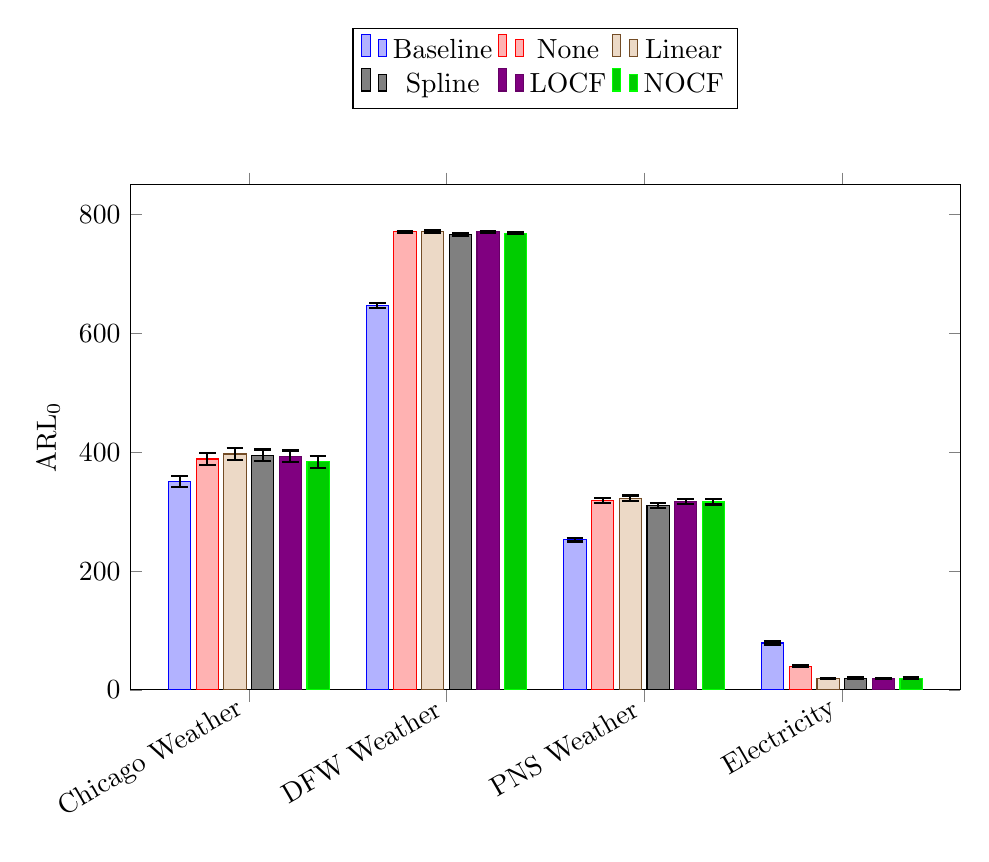
\begin{tikzpicture}
\begin{axis}[
    ybar,
    bar width=8pt, % Reduced to prevent bars from touching between categories
    width=\textwidth,
    height=8cm,
    ymin=0,
    ylabel={ARL$_0$},
    symbolic x coords={
        Chicago Weather,
        DFW Weather,
        PNS Weather,
        Electricity
    },
    xtick=data,
    x tick label style={rotate=30, anchor=east},
    enlarge x limits=0.2,
    legend style={
        at={(0.5,1.15)}, % Raised to avoid overlapping with high error bars
        anchor=south,
        legend columns=3 % Two neat rows of 3
    },
    % Corrected global error bar settings
    error bars/y dir=both,
    error bars/y explicit,
    error bars/error bar style={line width=0.8pt, black},
    error bars/error mark options={
        rotate=90,
        mark size=3pt,
        line width=0.8pt
    }
]

% Baseline
\addplot coordinates {
    (Chicago Weather,351.15) +- (0,9.414)
    (DFW Weather,647.166) +- (0,4.672)
    (PNS Weather,252.783) +- (0,2.872)
    (Electricity,78.979) +- (0,2.653)
};

% None
\addplot coordinates {
    (Chicago Weather,388.66) +- (0,9.832)
    (DFW Weather,771.227) +- (0,1.646)
    (PNS Weather,318.896) +- (0,4.394)
    (Electricity,39.772) +- (0,1.393)
};

% Linear
\addplot coordinates {
    (Chicago Weather,397.033) +- (0,9.866)
    (DFW Weather,771.632) +- (0,1.628)
    (PNS Weather,322.792) +- (0,4.309)
    (Electricity,19.576) +- (0,1.101)
};

% Spline
\addplot coordinates {
    (Chicago Weather,394.818) +- (0,9.835)
    (DFW Weather,766.846) +- (0,1.888)
    (PNS Weather,310.287) +- (0,4.314)
    (Electricity,19.706) +- (0,1.125)
};

% LOCF
\addplot coordinates {
    (Chicago Weather,393.157) +- (0,9.883)
    (DFW Weather,770.795) +- (0,1.749)
    (PNS Weather,317.519) +- (0,4.446)
    (Electricity,19.022) +- (0,1.047)
};

% NOCF
\addplot coordinates {
    (Chicago Weather,383.728) +- (0,9.731)
    (DFW Weather,768.772) +- (0,1.828)
    (PNS Weather,316.357) +- (0,4.329)
    (Electricity,19.841) +- (0,1.118)
};

\legend{Baseline, None, Linear, Spline, LOCF, NOCF}

\end{axis}
\end{tikzpicture}
\end{figure}


\begin{table}[htbp]
\centering
\caption{ARL$_0$ performance with standard deviation under 10\% missingness relative to baseline}
\label{tab:arl0_10pct_ext}
\resizebox{\textwidth}{!}{%
\begin{tabular}{lcccccccccccc}
\toprule
& \multicolumn{2}{c}{Baseline}
& \multicolumn{2}{c}{None}
& \multicolumn{2}{c}{Linear}
& \multicolumn{2}{c}{Spline}
& \multicolumn{2}{c}{LOCF}
& \multicolumn{2}{c}{NOCF} \\
\cmidrule(lr){2-3}
\cmidrule(lr){4-5}
\cmidrule(lr){6-7}
\cmidrule(lr){8-9}
\cmidrule(lr){10-11}
\cmidrule(lr){12-13}
\textbf{Dataset}
& \textbf{ARL$_0$} & \textbf{SD}
& \textbf{ARL$_0$} & \textbf{SD}
& \textbf{ARL$_0$} & \textbf{SD}
& \textbf{ARL$_0$} & \textbf{SD}
& \textbf{ARL$_0$} & \textbf{SD}
& \textbf{ARL$_0$} & \textbf{SD} \\
\midrule
Chicago Weather & 351.15 & 297.3739948 & 388.66 & 310.7066446 & 397.033 & 311.5507981 & 394.818 & 310.8683645 & 393.157 & 312.2944671 & 383.728 & 307.4908855 \\
DFW Weather     & 647.166 & 147.6277087 & 771.227 & 52.01233271 & 771.632 & 51.43360761 & 766.846 & 59.65538575 & 770.795 & 55.26884856 & 768.772 & 57.7450648 \\
PNS Weather     & 252.783 & 90.75284012 & 318.896 & 138.8530207 & 322.792 & 136.1585983 & 310.287 & 136.335586 & 317.519 & 140.4535255 & 316.357 & 136.8181741 \\
Electricity & 78.979 & 83.81632141 & 39.772 & 44.02272159 & 19.576 & 34.79797585 & 19.706 & 35.55246182 & 19.022 & 33.08589113  & 19.841 & 35.32287395 \\
\bottomrule
\end{tabular}}
\end{table}



\subsubsection{25\% Missingness}

Table~\ref{tab:arl0_25pct_ext} presents \ac{ARL}$_0$ performance under 25\% random row deletion.

\begin{figure}[htbp]
\centering
\caption{ARL$_0$ performance with standard error under 25\% missingness with extended reference timeframe for different imputation methods.}
\label{fig:arl0_25pct_ext}

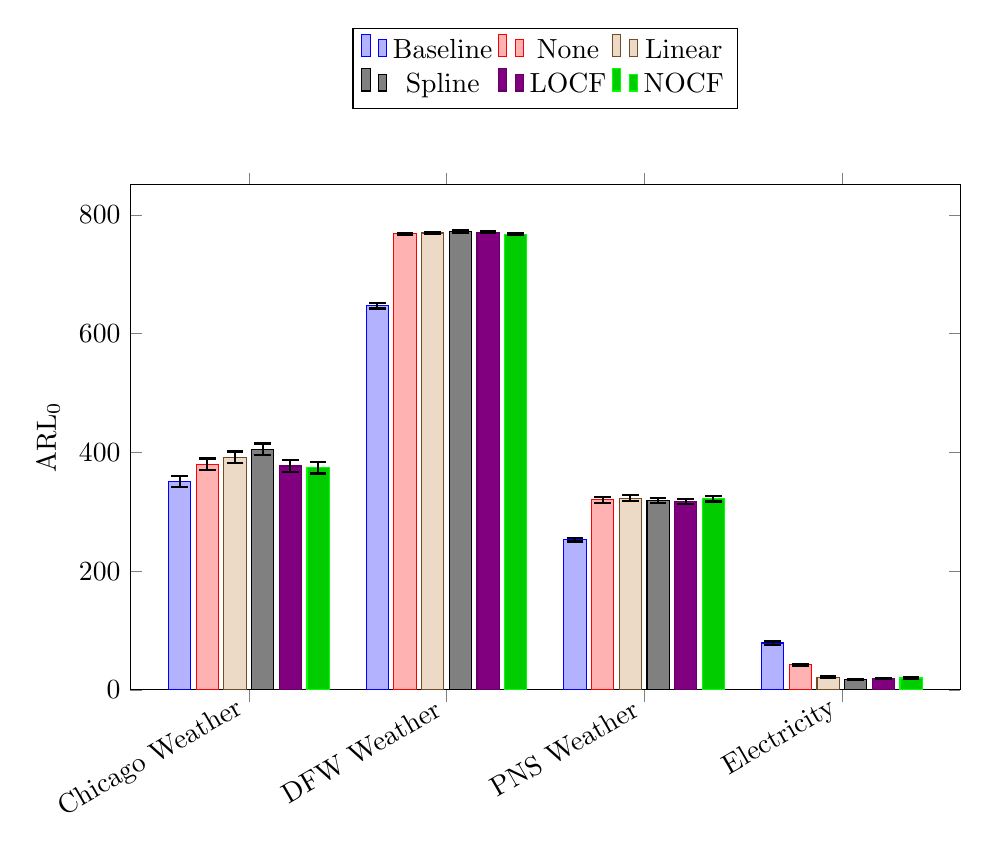
\begin{tikzpicture}
\begin{axis}[
    ybar,
    bar width=8pt,
    width=\textwidth,
    height=8cm,
    ymin=0,
    ylabel={ARL$_0$},
    symbolic x coords={
        Chicago Weather,
        DFW Weather,
        PNS Weather,
        Electricity
    },
    xtick=data,
    x tick label style={rotate=30, anchor=east},
    enlarge x limits=0.2,
    legend style={
        at={(0.5,1.15)},
        anchor=south,
        legend columns=3
    },
    % Corrected global error bar settings
    error bars/y dir=both,
    error bars/y explicit,
    error bars/error bar style={line width=0.8pt, black},
    error bars/error mark options={
        rotate=90,
        mark size=3pt,
        line width=0.8pt
    }
]

% Baseline
\addplot coordinates {
    (Chicago Weather,351.15) +- (0,9.414)
    (DFW Weather,647.166) +- (0,4.672)
    (PNS Weather,252.783) +- (0,2.872)
    (Electricity,78.979) +- (0,2.653)
};

% None
\addplot coordinates {
    (Chicago Weather,380.068) +- (0,9.739)
    (DFW Weather,768.251) +- (0,1.805)
    (PNS Weather,320.238) +- (0,4.798)
    (Electricity,42.344) +- (0,1.503)
};

% Linear
\addplot coordinates {
    (Chicago Weather,392.053) +- (0,9.803)
    (DFW Weather,769.843) +- (0,1.838)
    (PNS Weather,322.979) +- (0,4.809)
    (Electricity,21.67) +- (0,1.274)
};

% Spline
\addplot coordinates {
    (Chicago Weather,405.337) +- (0,9.886)
    (DFW Weather,772.335) +- (0,1.690)
    (PNS Weather,319.096) +- (0,4.602)
    (Electricity,17.93) +- (0,0.998)
};

% LOCF
\addplot coordinates {
    (Chicago Weather,377.197) +- (0,9.778)
    (DFW Weather,771.144) +- (0,1.733)
    (PNS Weather,317.68) +- (0,4.476)
    (Electricity,19.632) +- (0,1.103)
};

% NOCF
\addplot coordinates {
    (Chicago Weather,374.273) +- (0,9.747)
    (DFW Weather,767.663) +- (0,1.799)
    (PNS Weather,322.36) +- (0,4.833)
    (Electricity,20.077) +- (0,1.061)
};

\legend{Baseline, None, Linear, Spline, LOCF, NOCF}

\end{axis}
\end{tikzpicture}
\end{figure}



\begin{table}[htbp]
\centering
\caption{\ac{ARL}$_0$ performance with standard deviation under 25\% missingness.}
\label{tab:arl0_25pct_ext}
\resizebox{\textwidth}{!}{%
\begin{tabular}{lcccccccccccc}
\toprule
& \multicolumn{2}{c}{Baseline}
& \multicolumn{2}{c}{None}
& \multicolumn{2}{c}{Linear}
& \multicolumn{2}{c}{Spline}
& \multicolumn{2}{c}{LOCF}
& \multicolumn{2}{c}{NOCF} \\
\cmidrule(lr){2-3}
\cmidrule(lr){4-5}
\cmidrule(lr){6-7}
\cmidrule(lr){8-9}
\cmidrule(lr){10-11}
\cmidrule(lr){12-13}
\textbf{Dataset}
& \textbf{ARL$_0$} & \textbf{SD}
& \textbf{ARL$_0$} & \textbf{SD}
& \textbf{ARL$_0$} & \textbf{SD}
& \textbf{ARL$_0$} & \textbf{SD}
& \textbf{ARL$_0$} & \textbf{SD}
& \textbf{ARL$_0$} & \textbf{SD} \\
\midrule
Chicago Weather & 351.15 & 297.3739948 & 380.068 & 307.6500934 & 392.053 & 309.7007148 & 405.337 & 312.4373033 & 377.197 & 308.8738987 & 374.273 & 308.0035205 \\
DFW Weather     & 647.166 & 147.6277087 & 768.251 & 57.03083829 & 769.843	& 58.07718408 & 772.335 & 53.40935624	& 771.144 & 54.7774208 & 767.663 & 56.85817693 \\
PNS Weather     & 252.783 & 90.75284012 & 320.238 & 151.6175889 & 322.979 & 151.945062 & 319.096 & 145.397005 & 317.68 & 141.3939314 & 322.36 & 152.7370715 \\
Electricity & 78.979 & 83.81632141 & 42.344 & 47.50164281 & 21.67 & 40.27827503  & 17.93 & 31.53203719 & 19.632 & 34.8641088  & 20.077 & 33.52848386 \\
\bottomrule
\end{tabular}}
\end{table}

\subsubsection{50\% Missingness}

Table~\ref{tab:arl0_50pct_ext} presents \ac{ARL}$_0$ performance under 50\% random row deletion.

\begin{figure}[htbp]
\centering
\caption{ARL$_0$ performance with standard error under 50\% missingness with extended reference timeframe for different imputation methods.}
\label{fig:arl0_50pct_ext}

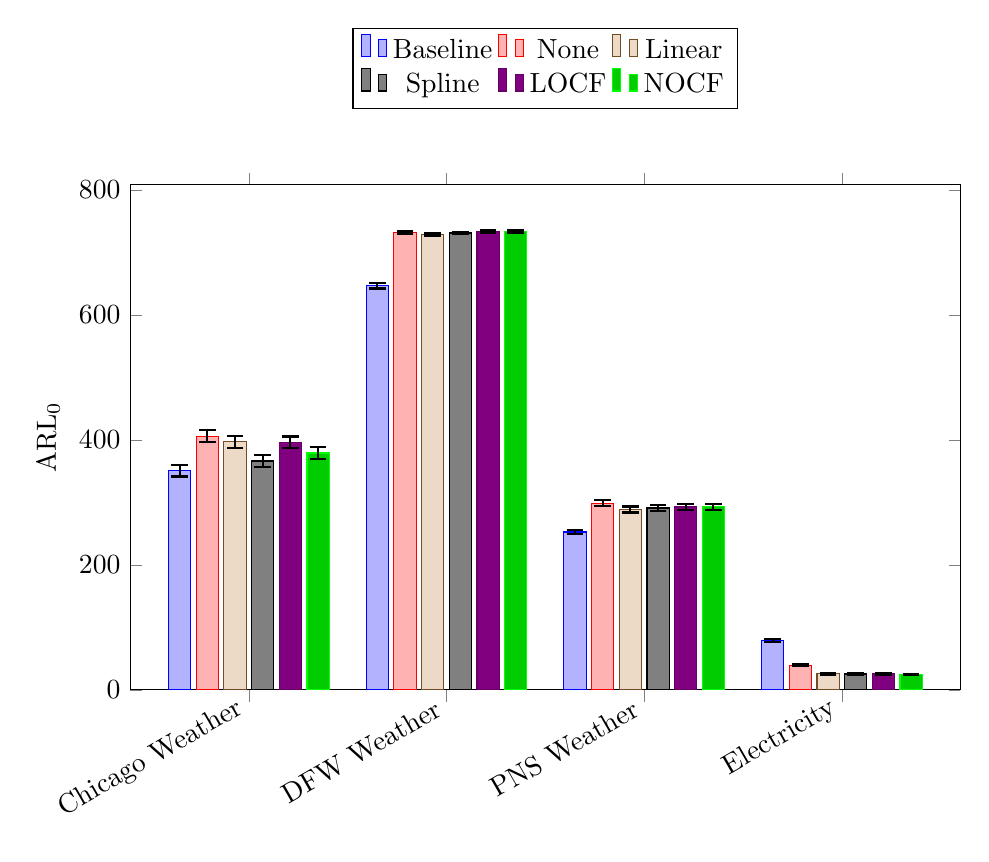
\begin{tikzpicture}
\begin{axis}[
    ybar,
    bar width=8pt,
    width=\textwidth,
    height=8cm,
    ymin=0,
    ylabel={ARL$_0$},
    symbolic x coords={
        Chicago Weather,
        DFW Weather,
        PNS Weather,
        Electricity
    },
    xtick=data,
    x tick label style={rotate=30, anchor=east},
    enlarge x limits=0.2,
    legend style={
        at={(0.5,1.15)},
        anchor=south,
        legend columns=3
    },
    % Corrected global error bar settings
    error bars/y dir=both,
    error bars/y explicit,
    error bars/error bar style={line width=0.8pt, black},
    error bars/error mark options={
        rotate=90,
        mark size=3pt,
        line width=0.8pt
    }
]

% Baseline
\addplot coordinates {
    (Chicago Weather,351.15) +- (0,9.414)
    (DFW Weather,647.166) +- (0,4.672)
    (PNS Weather,252.783) +- (0,2.872)
    (Electricity,78.979) +- (0,2.653)
};

% None
\addplot coordinates {
    (Chicago Weather,406.264) +- (0,9.443)
    (DFW Weather,732.018) +- (0,1.680)
    (PNS Weather,299.06) +- (0,4.912)
    (Electricity,39.644) +- (0,1.451)
};

% Linear
\addplot coordinates {
    (Chicago Weather,397.182) +- (0,9.467)
    (DFW Weather,728.53) +- (0,1.866)
    (PNS Weather,288.737) +- (0,4.683)
    (Electricity,25.675) +- (0,1.279)
};

% Spline
\addplot coordinates {
    (Chicago Weather,366.376) +- (0,9.382)
    (DFW Weather,731.254) +- (0,1.713)
    (PNS Weather,291.138) +- (0,4.717)
    (Electricity,25.514) +- (0,1.177)
};

% LOCF
\addplot coordinates {
    (Chicago Weather,396.247) +- (0,9.456)
    (DFW Weather,733.496) +- (0,1.652)
    (PNS Weather,292.784) +- (0,4.698)
    (Electricity,25.892) +- (0,1.311)
};

% NOCF
\addplot coordinates {
    (Chicago Weather,379.12) +- (0,9.414)
    (DFW Weather,733.528) +- (0,1.796)
    (PNS Weather,293.034) +- (0,4.748)
    (Electricity,24.923) +- (0,1.204)
};

\legend{Baseline, None, Linear, Spline, LOCF, NOCF}

\end{axis}
\end{tikzpicture}
\end{figure}


\begin{table}[htbp]
\centering
\caption{\ac{ARL}$_0$ performance with standard deviation under 50\% missingness.}
\label{tab:arl0_50pct_ext}
\resizebox{\textwidth}{!}{%
\begin{tabular}{lcccccccccccc}
\toprule
& \multicolumn{2}{c}{Baseline}
& \multicolumn{2}{c}{None}
& \multicolumn{2}{c}{Linear}
& \multicolumn{2}{c}{Spline}
& \multicolumn{2}{c}{LOCF}
& \multicolumn{2}{c}{NOCF} \\
\cmidrule(lr){2-3}
\cmidrule(lr){4-5}
\cmidrule(lr){6-7}
\cmidrule(lr){8-9}
\cmidrule(lr){10-11}
\cmidrule(lr){12-13}
\textbf{Dataset}
& \textbf{ARL$_0$} & \textbf{SD}
& \textbf{ARL$_0$} & \textbf{SD}
& \textbf{ARL$_0$} & \textbf{SD}
& \textbf{ARL$_0$} & \textbf{SD}
& \textbf{ARL$_0$} & \textbf{SD}
& \textbf{ARL$_0$} & \textbf{SD} \\
\midrule
Chicago Weather & 351.15 & 297.3739948 & 406.264 & 298.3934902 & 397.182 & 299.1356064 & 366.376 & 296.4089015 & 396.247 & 298.7183065 & 379.12 & 297.3940632 \\
DFW Weather     & 647.166 & 147.6277087 & 732.018 & 53.08545697 & 728.53 & 58.96077911 & 731.254 & 54.13991702 & 733.496 & 52.20831056 & 733.528 & 56.75269231 \\
PNS Weather     & 252.783 & 90.75284012 & 299.06 & 155.1944126 & 288.737 & 147.9167644 & 291.138 & 149.0095796 & 292.784 & 148.3663301 & 293.034 & 150.0635929 \\
Electricity & 78.979 & 83.81632141 & 39.644 & 45.82304022 & 25.675 & 40.40514758  & 25.514 & 37.16262726 & 25.892 & 41.43628001 & 24.923 & 38.06065796 \\
\bottomrule
\end{tabular}}
\end{table}


\subsection{Summary}

Taken together, these results demonstrate that interpolation primarily alters the temporal structure of the monitoring statistic rather than restoring its statistical properties. Differences in mean performance metrics generally remain within statistical uncertainty, while variability increases substantially under missingness. Apparent robustness is therefore largely illusory, driven by increased false-alarm activity rather than preserved detection power. In contrast, reference construction—particularly seasonal extension—provides a more effective mechanism for stabilizing monitoring behavior. These findings motivate the methodological recommendations discussed in Chapter~5.

\clearpage
\section{Discussion}

\subsection{Overview}

This chapter interprets the empirical findings presented in Chapter 4, contextualizing them within the broader literature on multivariate \ac{SPC} and \ac{IoT} monitoring. The discussion is structured around the research questions posed in Chapter 1, examining how missing data affects Hotelling's $T^2$ performance, the effectiveness of adaptation strategies, and the implications for practical deployment in environmental sensor networks.

The discussion is structured around the research questions posed in Chapter~1. It begins by examining the impact of missing data on statistical validity and \ac{ARL} performance (RQ1), followed by an evaluation of reference window extension and weighting schemes (RQ2). The role of interpolation and imputation methods is then assessed (RQ3), before identifying dataset characteristics that determine the practical suitability of Hotelling’s $T^2$ under missing data (RQ4). The chapter concludes with a comparison to theoretical expectations and prior literature, followed by a discussion of limitations and implications for practice and future research.

Particular emphasis is placed on the role of covariance stability, as shaped by inter-variable correlation structure, in mediating the robustness of Hotelling’s $T^2$ under missing data.
All interpretations account for statistical uncertainty in the estimated performance metrics, as discussed in Chapter~3, where uncertainty is quantified via standard errors and associated confidence intervals. Observed differences are therefore interpreted relative to this estimation uncertainty, ensuring that conclusions reflect structural effects rather than simulation variability.

\subsection{Interpretation of Key Findings}

This section interprets the empirical findings presented in Chapter 4 through the lens of the research questions defined in Section 1.8. Rather than reiterating numerical results, the discussion focuses on the mechanisms driving observed behavior and the implications for the practical use of Hotelling’s $T^2$ in IoT and environmental monitoring contexts.
Across all findings, differences in dataset behavior are interpreted through the lens of covariance preservation rather than missingness rate alone.


\subsubsection{RQ1: Effect of Missing Data Across Datasets}

How does missing data affect the run-length behavior (\ac{ARL}$_0$ and \ac{ARL}$_1$) of Hotelling’s $T^2$ across different IoT and environmental sensor datasets?

Across all datasets examined, missing data primarily affects Hotelling’s $T^2$ through increased instability of run-length distributions rather than through a uniform degradation of mean detection performance. Even when mean \ac{ARL}$_0$ values remain close to nominal targets, missing observations introduce variability in covariance estimation that manifests as heavy-tailed and highly dispersed run-length behavior. Importantly, the stability of mean \ac{ARL}$_0$ values falls within the range of statistical uncertainty as quantified by the standard error of the estimated \ac{ARL}$_0$, indicating that observed differences are not statistically significant but reflect stochastic variability. This indicates that missingness primarily affects variability rather than systematically biasing average performance. This effect is amplified in datasets exhibiting strong temporal dependence or latent nonstationarity, where successive monitoring statistics are no longer approximately independent.

The cross-dataset comparison reveals that the sensitivity of T² to missing data is not uniform but depends on the structural characteristics of the underlying process. In particular, datasets with stronger and more coherent inter-variable correlation exhibit more stable covariance estimation and correspondingly lower run-length dispersion, even under comparable levels of missingness. Environmental datasets with relatively smooth seasonal dynamics tolerate moderate levels of missingness more gracefully than processes characterized by regime switching or evolving variance structures. These findings indicate that missing data does not merely reduce information content, but fundamentally perturbs the statistical assumptions underpinning the T² chart, particularly those related to stable covariance estimation.

From a practical perspective, evaluating robustness based solely on average \ac{ARL} metrics—without accounting for their associated uncertainty—can be misleading. Stable monitoring performance requires not only appropriate mean behavior but also controlled dispersion of run-length distributions, especially in applications where false alarms carry significant operational cost.

\subsubsection{RQ2: Impact of Reference Data Quality}

How does missing or incomplete reference data influence false-alarm stability (\ac{ARL}$_0$) and detection performance (\ac{ARL}$_1$) of Hotelling’s $T^2$?

The results demonstrate that degradation of the reference dataset exerts a disproportionately large influence on monitoring robustness relative to missingness in the online monitoring stream. Because Hotelling’s $T^2$ relies on accurate estimation of the in-control mean vector and covariance matrix, any instability in the reference window propagates directly into the monitoring statistic and its control limits. Missing observations in the reference data reduce effective sample size and increase estimation variance, leading to inflated uncertainty in the inverse covariance matrix and, consequently, unstable signaling behavior. These effects exceed the expected statistical uncertainty of the simulation estimates, as defined by the standard error of the run-length metrics, indicating that the observed instability is statistically meaningful rather than attributable to sampling variability.


Importantly, the adverse effects of reference degradation do not persist when imputation-based reconstruction is applied. While interpolation may restore continuity in marginal series without fully recovering the true joint dependence structure required for reliable multivariate monitoring, charts calibrated on reconstructed reference data remain stable and maintain false-alarm rates close to their nominal \ac{ARL}$_0$ targets.

These findings underscore that robustness in Hotelling’s $T^2$ monitoring is governed primarily by the quality and representativeness of the reference dataset. Ensuring reference stability—through careful selection, extension, or updating of a representative covariance structure—emerges as a more effective robustness strategy.

\subsubsection{RQ3: Role of Imputation-Based Reconstruction}

To what extent do imputation-based reconstruction strategies stabilize or distort the run-length properties of Hotelling’s $T^2$ under increasing levels of missing data?

Imputation-based reconstruction plays an ambivalent role in the robustness of Hotelling’s $T^2$. On the one hand, commonly used methods such as linear interpolation and cubic splines preserve mean-shift detectability under moderate missingness by maintaining continuity in marginal trajectories. This explains the relative stability observed in minimal detectable shift factors across interpolation strategies and missingness levels. This apparent stability remains within statistical uncertainty bounds, indicating that interpolation does not significantly alter mean detection sensitivity. In this context, “no significant change” refers to differences that remain within the confidence bounds implied by the standard error of the estimated detection metrics.

On the other hand, interpolation implicitly imposes smoothness assumptions that alter the temporal and cross-variable dependence structure of the data. Carry-forward methods suppress short-term variability, while spline-based approaches may introduce artificial curvature or overshoot. These distortions do not significantly affect mean detection performance beyond statistical uncertainty, but they increase run-length dispersion and reduce reliability. Such effects are amplified in datasets with weak baseline correlation, where interpolation-induced smoothing further obscures already fragile dependence structures.

Consequently, interpolation should not be interpreted as a corrective mechanism that restores the statistical properties required for valid T² monitoring. Rather, it functions as a modeling assumption that trades one form of uncertainty (missingness) for another (structural distortion). Interpolation may be acceptable as a pragmatic stopgap under low to moderate missingness, but it cannot compensate for fundamental deficiencies in reference stability or structural nonstationarity.

\subsubsection{RQ4: Practical Suitability of Hotelling’s $T^2$ Under Missing Data}

Based on empirical run-length behavior, what characteristics distinguish datasets for which Hotelling’s $T^2$ remains practically usable under missing data from those for which it does not?

The findings suggest that the practical suitability of Hotelling’s $T^2$ under missing data depends less on the absolute level of missingness than on the stability and coherence of the underlying covariance structure.  Datasets characterized by relatively stationary dependence patterns and dominant seasonal dynamics remain amenable to T² monitoring when paired with robust reference construction strategies, such as seasonal reference extension. In these cases, missing data introduces manageable degradation that can be partially mitigated through careful preprocessing. In these cases, observed deviations in mean \ac{ARL}$_0$ remain within statistical uncertainty bounds defined by the standard error of the estimates, indicating that mean performance is not significantly affected.


In contrast, datasets exhibiting strong nonstationarity, regime switching, or time-varying variance structures challenge the foundational assumptions of Hotelling’s $T^2$. In such settings, interpolation smooths marginal behavior without capturing evolving multivariate relationships, leading to persistently unstable false-alarm behavior regardless of missingness level. These failures are not incidental but diagnostic of fundamental violations of the constant-covariance assumption underlying Hotelling’s $T^2$.

Taken together, these results support a qualitative suitability criterion: Hotelling’s $T^2$ remains practically usable under missing data when the reference covariance structure is stable and representative of ongoing process dynamics. When this condition is violated, alternative monitoring frameworks that explicitly model nonstationarity or dynamic dependence should be preferred.

\subsubsection{Synthesis}

Across all research questions, a consistent conclusion emerges: the robustness of Hotelling’s $T^2$ under missing data is governed primarily by the preservation of a stable and representative covariance structure. Missing data, interpolation, and reference degradation all exert their influence through this mechanism. While preprocessing and reconstruction can mitigate superficial data loss, they cannot compensate for weak correlation structure or structural nonstationarity. These findings clarify both the limits and the continued relevance of Hotelling’s $T^2$, demonstrating that robustness must be assessed through both mean performance and its associated uncertainty.
Across all findings, statistical significance is assessed relative to estimation uncertainty, confirming that variability effects dominate over systematic shifts in mean performance.

\subsection{Cross-Dataset Generalizability}

\subsubsection{Consistency of Findings Across Datasets}

Across datasets, adaptation method effectiveness exhibited moderate consistency across the four datasets.

Across datasets, reference window extension strategies—particularly those incorporating seasonal structure—consistently outperform interpolation-only approaches in terms of false-alarm stability. However, the magnitude of improvement varies across datasets and is primarily driven by differences in dimensionality, temporal dependence, seasonality strength, and covariance stability. Hybrid approaches combining reference extension with interpolation generally exhibit more stable behavior than single-method adaptations, although their effectiveness remains dependent on dataset-specific characteristics.

Taken together, these patterns indicate that generalizability is constrained less by domain and more by covariance stability and temporal structure. Observed differences across datasets consistently exceed statistical uncertainty, confirming that these effects are driven by structural properties rather than simulation variability.


\subsubsection{Dataset Characteristics as Moderating Factors}

Analysis of dataset sensitivity indicates that the following characteristics moderate adaptation effectiveness:

\paragraph{Dimensionality} Datasets with higher dimensionality exhibited greater sensitivity to missingness, reflecting increased instability in covariance estimation and matrix inversion as the effective sample size decreased.


\paragraph{Autocorrelation} Datasets with strong autocorrelation exhibited improved performance under imputation-based reconstruction, as temporal smoothness assumptions better preserved the evolving multivariate dependence structure required for stable Hotelling’s $T^2$ monitoring.

\paragraph{Seasonality Strength} The effectiveness of seasonal reference extension increased with the strength and regularity of seasonal patterns in the data, as recurring structure improved covariance representativeness and reduced estimation variance.

\paragraph{Correlation Structure}
Datasets with stronger inter-variable correlation exhibited greater robustness to missingness, reflecting more stable covariance estimation and reduced sensitivity to effective sample size reductions.


\subsection{Comparison with Theoretical Expectations}

\subsubsection{Alignment with Classical SPC Theory}

Under complete data conditions, observed \ac{ARL}$_0$ values closely matched theoretical predictions assuming multivariate normality. This validates the applicability of Hotelling's $T^2$ to environmental data. Observed deviations from theoretical \ac{ARL}$_0$ values are small relative to statistical uncertainty under near-complete data, but increase substantially under missingness.

These deviations are primarily attributable to autocorrelation, which inflates false-alarm rates \cite{Venkatasubramanian2003}, and to limited sample sizes in the reference windows, which increase estimation uncertainty.

These assumptions implicitly rely on stable covariance structure, explaining the sensitivity observed under weak correlation and nonstationarity.


\subsubsection{Relationship to Modern Robust Methods}

Recent advances by \cite{Xie2024} (EWMA-Q) and \cite{Xie2023} (\ac{NDPM}) provide distribution-free alternatives that complement classical $T^2$ under conditions of pronounced nonstationarity, high missingness, or unstable covariance structure.


The findings suggest that for missingness levels below approximately 20\%, classical $T^2$ remains competitive when supported by appropriate reference construction and moderate interpolation. Beyond moderate missingness, transition to robust or adaptive monitoring frameworks becomes advisable, particularly when reference stability cannot be maintained. Nevertheless, the computational simplicity and interpretability of $T^2$ justify its continued use in low- to moderate-missingness environmental monitoring contexts where reference data remain stable.


\subsection{Limitations and Threats to Validity}

\subsubsection{Internal Validity}

\subsubsection{Missing Data Mechanisms}

This study imposed \ac{MCAR} missingness, which may not reflect all real-world patterns. In practice, missing data often exhibit more complex patterns. Sensor outages may cluster temporally (\ac{MAR}), missingness may correlate with extreme values (\ac{MNAR}), and network failures can affect multiple sensors simultaneously.

Future work should explicitly model structured and outcome-dependent missingness processes.

Evaluating MNAR mechanisms would require explicit modeling of missingness processes and lies beyond the scope of this work, but represents a critical direction for future research.

\subsubsection{Sampling Variability}

Choice of random seed for missingness simulation may introduce variability. While multiple runs were averaged, residual sampling variability may still affect precision, particularly for heavy-tailed run-length distributions where convergence is slower.

While confidence intervals were not explicitly reported in all result tables, the magnitude of observed effects relative to the standard error of the estimates suggests that the main conclusions are robust to simulation noise.

\subsubsection{Monitoring Window Selection Implementation}

Choice of monitoring window size and update frequency may influence detection performance. Fixed window sizes were used for consistency, but adaptive windowing could yield different results. The window selection was constrained by data availability within the datasets that lacked certain periods of high-frequency data.


\subsubsection{External Validity}

\subsubsection{Dataset Representativeness}

Four datasets provide moderate coverage of environmental monitoring scenarios, but may not generalize to industrial process monitoring, high-frequency sensor networks ($>$1 Hz), or extremely high-dimensional systems ($>$20 variables).

\subsubsection{Shift Detection Evaluation}

Minimal detectable shift analysis assumed specific shift types: mean shift. Results may differ for gradual drifts, transient anomalies, multimodal shifts.

\subsubsection{Construct Validity}

\ac{ARL} metrics assume stationarity and ergodicity, which may be violated in long-running deployments subject to sensor drift, environmental regime changes.

\subsubsection{Dataset Completeness Limitations}

All datasets used were pre-processed to remove existing missing data, which may not reflect real-world sensor network conditions where missingness patterns are complex and non-random. This could limit the ecological validity of the findings.
Additionally the datasets lacked high frequency data for certain periods which limited the ability to simulate high frequency missingness patterns. 


\clearpage
\section{Practical Implications}

This chapter translates the empirical findings of the thesis into actionable design guidance for real-world deployment. While previous chapters focused on statistical behavior and theoretical robustness, the emphasis here shifts toward practicability: how Hotelling’s $T^2$ can be effectively implemented, maintained, and evaluated in operational \ac{IoT} monitoring systems under imperfect data conditions.

The recommendations presented are derived directly from the observed relationships between missing data, covariance stability, and run-length behavior. Rather than proposing new methods, this chapter provides structured guidance on when classical $T^2$ is appropriate, how it should be configured, and when alternative approaches should be considered.

\subsubsection{For Practitioners}

The following guidelines are intended for practitioners deploying multivariate monitoring systems in real-world \ac{IoT} environments, where missing data, nonstationarity, and resource constraints are common. The recommendations emphasize robustness, interpretability, and operational feasibility rather than theoretical optimality.

\subsubsection{Deployment Guidelines}

Deployment of Hotelling’s $T^2$ under missing data conditions should be structured across three stages: pre-deployment assessment, implementation design, and ongoing monitoring and maintenance.

\begin{enumerate}
	\item \textbf{Pre-deployment assessment:}
	\begin{itemize}
		\item Characterize expected missingness patterns, including frequency, clustering, and potential correlation with extreme values.
		\item Evaluate dataset characteristics against suitability criteria: assess covariance stability, strength of inter-variable correlations, seasonality, and autocorrelation.
		\item Validate normality assumptions and approximate independence of monitoring statistics, noting that strong temporal dependence or nonstationarity may compromise performance.
	\end{itemize}
    These steps are critical, as the results of this thesis show that monitoring performance is governed primarily by covariance stability rather than missingness level alone.
	
	\item \textbf{Implementation recommendations:}
	\begin{itemize}
		\item Apply interpolation cautiously: use linear or cubic spline interpolation for moderate missingness where marginal continuity is sufficient, but avoid over-reliance in weakly correlated or nonstationary datasets.
		\item Prefer reference window extension strategies, particularly seasonal reference extension when strong seasonal patterns exist, to stabilize covariance estimation.
		\item Implement periodic re-estimation of reference statistics to maintain a representative covariance structure as process dynamics evolve.
		\item Consider hybrid approaches combining reference extension and interpolation for improved false-alarm stability, while monitoring dataset-specific characteristics.
	\end{itemize}
    Consistent with the empirical findings, reference construction strategies have a greater impact on robustness than interpolation alone, and should therefore be prioritized in system design.
	
	\item \textbf{Monitoring and maintenance:}
	\begin{itemize}
		\item Continuously track \ac{ARL}$_0$ and run-length distribution dispersion against target values, not just mean performance.
		\item Flag datasets with unstable covariance structure or weak inter-variable correlation for alternative monitoring methods.
		\item Combine $T^2$ with complementary robust or adaptive methods (e.g., EWMA-Q or NDPM) when missingness exceeds approximately 20\% or reference stability cannot be maintained.
	\end{itemize}
    Ongoing evaluation of variability is essential, as stable mean \ac{ARL} values may mask deteriorating reliability due to increased run-length dispersion.
\end{enumerate}

\subsubsection{Cost-Benefit Considerations}

From a system design perspective, the choice of monitoring method involves a trade-off between computational simplicity, interpretability, and robustness under imperfect data.

Hotelling's $T^2$ remains competitive under low-to-moderate missingness, particularly when covariance stability is preserved. Its advantages include:

\begin{itemize}
	\item Computational efficiency and real-time applicability in resource-constrained IoT environments.
	\item Interpretability and transparency, facilitating regulatory compliance and actionable decision-making.
	\item Suitability in infrastructures where implementing advanced machine learning or robust adaptive frameworks is impractical.
\end{itemize}

Performance trade-offs remain manageable when the reference dataset is representative and covariance stability is maintained. However, when these conditions are violated—particularly under high missingness or nonstationarity—the reliability of $T^2$ deteriorates rapidly, and the use of robust or adaptive monitoring frameworks becomes necessary.

Overall, these guidelines reinforce the central conclusion of this thesis: effective deployment of Hotelling’s $T^2$ under missing data depends less on correcting missing observations and more on maintaining a stable and representative covariance structure. Practical robustness is therefore achieved through careful reference design, continuous monitoring of variability, and informed method selection.

\clearpage
\section{Conclusion And Future Work}

\noindent The findings presented in this chapter are based on the analysis of only four datasets and are therefore most applicable to datasets with similar statistical and structural characteristics. While the selected datasets were chosen to represent a range of conditions relevant to IoT and environmental sensor networks, caution is warranted when extending these conclusions to other contexts. Differences in dependence structures, missingness mechanisms, nonstationarity, or domain-specific factors may lead to different monitoring behavior. Consequently, the results should be interpreted as indicative rather than universally generalizable, and further validation across a broader spectrum of datasets is recommended.

\subsection{Summary of Key Findings}

This study investigated the robustness of Hotelling’s $T^2$ monitoring under missing data in \ac{IoT} and environmental sensor networks. Across four diverse datasets and multiple adaptation strategies, several consistent insights emerged.

First, Hotelling’s $T^2$ exhibits conditional robustness under missing data. The chart remains reliable up to moderate missingness levels (approximately 20--25\%), provided that the reference covariance structure is stable. Beyond this threshold, the underlying statistical assumptions deteriorate, and neither imputation nor reference extension can fully restore theoretical \ac{ARL}$_0$ behavior.

Second, monitoring robustness is governed primarily by the quality of the reference dataset rather than by online data reconstruction. Seasonal reference extension consistently stabilizes covariance estimation and reduces false-alarm variability, even under substantial missingness.

Third, imputation methods provide limited benefits. While linear, spline, and carry-forward approaches preserve marginal continuity and maintain mean-shift detectability, they fail to recover the multivariate dependency structure required for reliable covariance estimation. As a result, imputation cannot correct the structural distortions introduced by missing data.

Fourth, hybrid strategies combining reference extension with imputation yield only modest improvements and remain dependent on the robustness of the reference dataset. imputation alone cannot compensate for deficiencies in covariance estimation.

Fifth, dataset characteristics play a decisive role in determining performance. Strong inter-variable correlation, stationary covariance structures, and pronounced seasonality improve tolerance to missing data, whereas nonstationarity, regime shifts, and weak correlation amplify instability.

Finally, run-length dispersion emerges as a critical metric for evaluating monitoring performance. Stable mean \ac{ARL} values may conceal substantial increases in variability, indicating that robustness must be assessed through both average behavior and its associated uncertainty.

Taken together, these results clarify that Hotelling’s $T^2$ exhibits \textit{conditional, not inherent, robustness} under missing data. This distinction is essential for both practitioners and researchers designing multivariate monitoring systems.

\subsection{Implications for Practical Deployment}

From a practitioner perspective, the results provide clear operational guidance. For missingness levels below approximately 20\%, Hotelling’s $T^2$ remains broadly usable when supported by standard preprocessing and periodic reference updates. In the intermediate range of 20--35\% missingness, seasonal reference extension becomes essential, and monitoring results should be interpreted with increased caution due to rising variability. Beyond approximately 35--40\% missingness, classical $T^2$ loses reliability, and alternative robust or adaptive monitoring frameworks should be considered.

In all cases, practitioners should evaluate covariance stability and run-length dispersion alongside mean \ac{ARL} metrics. Hybrid strategies may offer incremental improvements, but only when the underlying reference dataset remains stable and representative.

Practitioners should also track covariance stability and run-length dispersion, not just mean \ac{ARL} metrics, and consider hybrid strategies only when reference robustness is ensured.

\subsection{Contributions to SPC Literature}

\subsubsection{Classical Methods in Modern Contexts}

Despite decades of methodological evolution, Hotelling’s $T^2$ remains relevant in modern IoT monitoring contexts. This study demonstrates that classical methods retain practical value when applied with an awareness of their limitations and supported by appropriate adaptations, including reference window extension, careful preprocessing, and dataset-specific evaluation of covariance stability.

\subsubsection{Bridging to Robust and Adaptive Methods}

The findings complement modern distribution-free or adaptive monitoring methods \cite{Xie2023,Xie2024}. While classical $T^2$ is competitive under low-to-moderate missingness, robust frameworks are better suited to high-missingness or nonstationary regimes. This study establishes the boundary conditions for classical $T^2$, facilitating informed method selection.

\subsection{Future Research Directions}

Several directions for future research emerge from this work. Extending the analysis to more realistic missingness mechanisms, such as \ac{MAR} and \ac{MNAR}, would improve applicability to real-world sensor networks where missingness is often structured or outcome-dependent. In parallel, the development of adaptive control limits that respond dynamically to missingness levels, imputatio strategies, and real-time \ac{ARL}$_0$ estimates represents a promising avenue for improving robustness.

Further research should also explore multivariate imputation techniques that explicitly preserve cross-variable dependence, moving beyond univariate imputation approaches. Hybrid monitoring frameworks that integrate $T^2$ with complementary anomaly detection methods may offer improved performance across diverse conditions, particularly under high missingness or nonstationarity.

Finally, incorporating online learning mechanisms to update reference statistics in streaming environments could address concept drift and evolving covariance structures. Systematic parameter sensitivity studies would also help clarify how design choices—such as subgroup size, covariance estimation method, and control limits—interact with dataset characteristics to influence monitoring performance.

\subsection{Final Remarks}

This study underscores that robustness in multivariate monitoring is inherently contextual and conditional. Hotelling’s $T^2$ is not universally resilient to missing data; rather, its performance depends critically on reference quality, covariance stability, and dataset characteristics. By identifying the limits of imputatio, emphasizing the central role of reference construction, and providing empirically grounded thresholds for missingness, this work offers actionable guidance for both practitioners and researchers.

Classical SPC methods can therefore continue to provide value in modern, imperfect-data environments when applied with a nuanced understanding of their assumptions and supported by appropriate preprocessing and reference management strategies.


\newpage
\printbibliography[title={REFERENCES}, heading=bibintoc]

\captionsetup{list=no}

\chapter{Definition of iterations}
\begin{table}[!htbp]
\centering
\caption{Comparison of Number of iterations on DFW dataset}
\begin{tabular}{lccc}
\toprule
Number of Runs & 500 & 1000  & 10000 \\
Average Run Length & 656.208 & 647.166 & 648.7816 \\
ARL Standard deviation & 147.0588227 & 147.6277087 & 147.6697489 \\
relative humidity factor mean & 3.97834 & 3.978538 & 3.979847 \\
relative humidity factor sd & 0.04360334 & 0.04504859 & 0.04365471 \\
station level pressure factor mean & 5.128857 & 5.135928 & 5.135491 \\
station level pressure factor sd & 0.04266235 & 0.04148334 & 0.04143443 \\
temperature factor mean & 3.422016 & 3.424553 & 3.424741 \\
temperature factor sd & 0.03372063 & 0.0335356 & 0.03405425 \\
wind speed factor mean & 5.923936 & 5.925634 & 5.926827 \\
wind speed factor sd & 0.05439861 & 0.05426472 & 0.05345255 \\
\bottomrule
\end{tabular}
\end{table}

\chapter{Tables for factor detection for PNS dataset}
% PNS drop0
\begin{table}[!htbp]
\centering
\caption{Minimal detectable shift under 0\% missingness (PNS).}
\resizebox{\textwidth}{!}{%
\begin{tabular}{lcccccccccccc}
\toprule
& \multicolumn{2}{c}{Baseline} & \multicolumn{2}{c}{None} & \multicolumn{2}{c}{Linear} & \multicolumn{2}{c}{Spline} & \multicolumn{2}{c}{Locf} & \multicolumn{2}{c}{Nocb}\\
\textbf{Dataset} & \textbf{Factor} & \textbf{SD} & \textbf{Factor} & \textbf{SD} & \textbf{Factor} & \textbf{SD} & \textbf{Factor} & \textbf{SD} & \textbf{Factor} & \textbf{SD} & \textbf{Factor} & \textbf{SD}\\
\midrule
dew point temperature & 0.9024199 & 0.0389189 &  &  & 0.9024199 & 0.0389189 & 0.9036914 & 0.03754379 & 0.9042275 & 0.03853153 & 0.9026172 & 0.03847128 \\
relative humidity & 1.0982461 & 0.03508391 &  &  & 1.0982461 & 0.03508391 & 1.099458 & 0.03459863 & 1.1001992 & 0.03421246 & 1.0964678 & 0.03480853 \\
temperature & 0.7265938 & 0.01842758 &  &  & 0.7265938 & 0.01842758 & 0.7270977 & 0.0175918 & 0.7271543 & 0.01817727 & 0.7254512 & 0.01818226 \\
wet bulb temperature & 0.6360264 & 0.03216921 &  &  & 0.6360264 & 0.03216921 & 0.637375 & 0.03095878 & 0.6370859 & 0.03134408 & 0.6343018 & 0.03258845 \\
\bottomrule
\end{tabular}}
\end{table}


\begin{figure}[!htbp]
\centering
\caption{Minimal detectable shift under 0\% missingness (PNS).}
\label{fig:PNS_0}
\begin{tikzpicture}
\begin{axis}[ybar, bar width=8pt, width=\textwidth, height=7cm, ymin=0,
ylabel={Minimal Detectable Shift (Factor)},
symbolic x coords={dew point temperature,relative humidity,temperature,wet bulb temperature},
xtick=data, x tick label style={rotate=30, anchor=east},
legend style={at={(0.5,1.05)}, anchor=south, legend columns=6},
error bars/.cd, y dir=both, y explicit]

\addplot coordinates {
(dew point temperature,0.9024199) +- (0,0.0389189)
(relative humidity,1.0982461) +- (0,0.03508391)
(temperature,0.7265938) +- (0,0.01842758)
(wet bulb temperature,0.6360264) +- (0,0.03216921)
};

\addplot coordinates {
(dew point temperature,0.9024199) +- (0,0.0389189)
(relative humidity,1.0982461) +- (0,0.03508391)
(temperature,0.7265938) +- (0,0.01842758)
(wet bulb temperature,0.6360264) +- (0,0.03216921)
};

\addplot coordinates {
(dew point temperature,0.9036914) +- (0,0.03754379)
(relative humidity,1.099458) +- (0,0.03459863)
(temperature,0.7270977) +- (0,0.0175918)
(wet bulb temperature,0.637375) +- (0,0.03095878)
};

\addplot coordinates {
(dew point temperature,0.9042275) +- (0,0.03853153)
(relative humidity,1.1001992) +- (0,0.03421246)
(temperature,0.7271543) +- (0,0.01817727)
(wet bulb temperature,0.6370859) +- (0,0.03134408)
};

\addplot coordinates {
(dew point temperature,0.9026172) +- (0,0.03847128)
(relative humidity,1.0964678) +- (0,0.03480853)
(temperature,0.7254512) +- (0,0.01818226)
(wet bulb temperature,0.6343018) +- (0,0.03258845)
};
\legend{Baseline, None, Linear, Spline, LOCF, NOCF}
\end{axis}
\end{tikzpicture}
\end{figure}


% PNS drop10
\begin{table}[!htbp]
\centering
\caption{Minimal detectable shift under 10\% missingness (PNS).}
\resizebox{\textwidth}{!}{%
\begin{tabular}{lcccccccccccc}
\toprule
& \multicolumn{2}{c}{Baseline} & \multicolumn{2}{c}{None} & \multicolumn{2}{c}{Linear} & \multicolumn{2}{c}{Spline} & \multicolumn{2}{c}{Locf} & \multicolumn{2}{c}{Nocb}\\
\textbf{Dataset} & \textbf{Factor} & \textbf{SD} & \textbf{Factor} & \textbf{SD} & \textbf{Factor} & \textbf{SD} & \textbf{Factor} & \textbf{SD} & \textbf{Factor} & \textbf{SD} & \textbf{Factor} & \textbf{SD}\\
\midrule
dew point temperature & 0.9024199 & 0.0389189 & 0.9035449 & 0.03947883 & 0.9006182 & 0.03822277 & 0.9036514 & 0.03748649 & 0.9007246 & 0.03914525 & 0.9010947 & 0.03846015 \\
relative humidity & 1.0982461 & 0.03508391 & 1.0995381 & 0.03272502 & 1.0970215 & 0.03486093 & 1.0973555 & 0.03581421 & 1.0980977 & 0.03537715 & 1.0977031 & 0.03537813 \\
temperature & 0.7265938 & 0.01842758 & 0.7264668 & 0.01782647 & 0.7260811 & 0.0176252 & 0.7257539 & 0.01755151 & 0.7257471 & 0.01773943 & 0.7250068 & 0.01763558 \\
wet bulb temperature & 0.6360264 & 0.03216921 & 0.6356543 & 0.03118701 & 0.636876 & 0.03127704 & 0.6347773 & 0.03295163 & 0.6352178 & 0.03132946 & 0.634875 & 0.0327871 \\
\bottomrule
\end{tabular}}
\end{table}


\begin{figure}[!htbp]
\centering
\caption{Minimal detectable shift under 10\% missingness (PNS).}
\label{fig:PNS_10}
\begin{tikzpicture}
\begin{axis}[ybar, bar width=8pt, width=\textwidth, height=7cm, ymin=0,
ylabel={Minimal Detectable Shift (Factor)},
symbolic x coords={dew point temperature,relative humidity,temperature,wet bulb temperature},
xtick=data, x tick label style={rotate=30, anchor=east},
legend style={at={(0.5,1.05)}, anchor=south, legend columns=6},
error bars/.cd, y dir=both, y explicit]

\addplot coordinates {
(dew point temperature,0.9024199) +- (0,0.0389189)
(relative humidity,1.0982461) +- (0,0.03508391)
(temperature,0.7265938) +- (0,0.01842758)
(wet bulb temperature,0.6360264) +- (0,0.03216921)
};

\addplot coordinates {
(dew point temperature,0.9035449) +- (0,0.03947883)
(relative humidity,1.0995381) +- (0,0.03272502)
(temperature,0.7264668) +- (0,0.01782647)
(wet bulb temperature,0.6356543) +- (0,0.03118701)
};

\addplot coordinates {
(dew point temperature,0.9006182) +- (0,0.03822277)
(relative humidity,1.0970215) +- (0,0.03486093)
(temperature,0.7260811) +- (0,0.0176252)
(wet bulb temperature,0.636876) +- (0,0.03127704)
};

\addplot coordinates {
(dew point temperature,0.9036514) +- (0,0.03748649)
(relative humidity,1.0973555) +- (0,0.03581421)
(temperature,0.7257539) +- (0,0.01755151)
(wet bulb temperature,0.6347773) +- (0,0.03295163)
};

\addplot coordinates {
(dew point temperature,0.9007246) +- (0,0.03914525)
(relative humidity,1.0980977) +- (0,0.03537715)
(temperature,0.7257471) +- (0,0.01773943)
(wet bulb temperature,0.6352178) +- (0,0.03132946)
};

\addplot coordinates {
(dew point temperature,0.9010947) +- (0,0.03846015)
(relative humidity,1.0977031) +- (0,0.03537813)
(temperature,0.7250068) +- (0,0.01763558)
(wet bulb temperature,0.634875) +- (0,0.0327871)
};
\legend{Baseline, None, Linear, Spline, LOCF, NOCF}
\end{axis}
\end{tikzpicture}
\end{figure}


% PNS drop25
\begin{table}[!htbp]
\centering
\caption{Minimal detectable shift under 25\% missingness (PNS).}
\resizebox{\textwidth}{!}{%
\begin{tabular}{lcccccccccccc}
\toprule
& \multicolumn{2}{c}{Baseline} & \multicolumn{2}{c}{None} & \multicolumn{2}{c}{Linear} & \multicolumn{2}{c}{Spline} & \multicolumn{2}{c}{Locf} & \multicolumn{2}{c}{Nocb}\\
\textbf{Dataset} & \textbf{Factor} & \textbf{SD} & \textbf{Factor} & \textbf{SD} & \textbf{Factor} & \textbf{SD} & \textbf{Factor} & \textbf{SD} & \textbf{Factor} & \textbf{SD} & \textbf{Factor} & \textbf{SD}\\
\midrule
dew point temperature & 0.9024199 & 0.0389189 & 0.9076953 & 0.03829504 & 0.9072305 & 0.03802324 & 0.9112842 & 0.03883786 & 0.9070742 & 0.03814308 & 0.907918 & 0.03825413 \\
relative humidity & 1.0982461 & 0.03508391 & 1.1032578 & 0.03587474 & 1.103418 & 0.03580926 & 1.1053252 & 0.03589077 & 1.1059346 & 0.0361843 & 1.1048379 & 0.03676155 \\
temperature & 0.7265938 & 0.01842758 & 0.7272734 & 0.0189484 & 0.7279746 & 0.01892251 & 0.7290273 & 0.01815416 & 0.7281729 & 0.01863495 & 0.7284092 & 0.01923886 \\
wet bulb temperature & 0.6360264 & 0.03216921 & 0.6394346 & 0.03138913 & 0.6399971 & 0.03270398 & 0.6441338 & 0.03262665 & 0.6411641 & 0.03357582 & 0.6413506 & 0.03269738 \\
\bottomrule
\end{tabular}}
\end{table}


\begin{figure}[!htbp]
\centering
\caption{Minimal detectable shift under 25\% missingness (PNS).}
\label{fig:PNS_25}
\begin{tikzpicture}
\begin{axis}[ybar, bar width=8pt, width=\textwidth, height=7cm, ymin=0,
ylabel={Minimal Detectable Shift (Factor)},
symbolic x coords={dew point temperature,relative humidity,temperature,wet bulb temperature},
xtick=data, x tick label style={rotate=30, anchor=east},
legend style={at={(0.5,1.05)}, anchor=south, legend columns=6},
error bars/.cd, y dir=both, y explicit]

\addplot coordinates {
(dew point temperature,0.9024199) +- (0,0.0389189)
(relative humidity,1.0982461) +- (0,0.03508391)
(temperature,0.7265938) +- (0,0.01842758)
(wet bulb temperature,0.6360264) +- (0,0.03216921)
};

\addplot coordinates {
(dew point temperature,0.9076953) +- (0,0.03829504)
(relative humidity,1.1032578) +- (0,0.03587474)
(temperature,0.7272734) +- (0,0.0189484)
(wet bulb temperature,0.6394346) +- (0,0.03138913)
};

\addplot coordinates {
(dew point temperature,0.9072305) +- (0,0.03802324)
(relative humidity,1.103418) +- (0,0.03580926)
(temperature,0.7279746) +- (0,0.01892251)
(wet bulb temperature,0.6399971) +- (0,0.03270398)
};

\addplot coordinates {
(dew point temperature,0.9112842) +- (0,0.03883786)
(relative humidity,1.1053252) +- (0,0.03589077)
(temperature,0.7290273) +- (0,0.01815416)
(wet bulb temperature,0.6441338) +- (0,0.03262665)
};

\addplot coordinates {
(dew point temperature,0.9070742) +- (0,0.03814308)
(relative humidity,1.1059346) +- (0,0.0361843)
(temperature,0.7281729) +- (0,0.01863495)
(wet bulb temperature,0.6411641) +- (0,0.03357582)
};

\addplot coordinates {
(dew point temperature,0.907918) +- (0,0.03825413)
(relative humidity,1.1048379) +- (0,0.03676155)
(temperature,0.7284092) +- (0,0.01923886)
(wet bulb temperature,0.6413506) +- (0,0.03269738)
};
\legend{Baseline, None, Linear, Spline, LOCF, NOCF}
\end{axis}
\end{tikzpicture}
\end{figure}


% PNS drop50
\begin{table}[!htbp]
\centering
\caption{Minimal detectable shift under 50\% missingness (PNS).}
\resizebox{\textwidth}{!}{%
\begin{tabular}{lcccccccccccc}
\toprule
& \multicolumn{2}{c}{Baseline} & \multicolumn{2}{c}{None} & \multicolumn{2}{c}{Linear} & \multicolumn{2}{c}{Spline} & \multicolumn{2}{c}{Locf} & \multicolumn{2}{c}{Nocb}\\
\textbf{Dataset} & \textbf{Factor} & \textbf{SD} & \textbf{Factor} & \textbf{SD} & \textbf{Factor} & \textbf{SD} & \textbf{Factor} & \textbf{SD} & \textbf{Factor} & \textbf{SD} & \textbf{Factor} & \textbf{SD}\\
\midrule
dew point temperature & 0.9024199 & 0.0389189 & 0.9105176 & 0.04576553 & 0.9122617 & 0.04350996 & 0.9101807 & 0.04321145 & 0.9105508 & 0.04530957 & 0.9099219 & 0.04407067 \\
relative humidity & 1.0982461 & 0.03508391 & 1.1002031 & 0.04150854 & 1.1025 & 0.04350211 & 1.1003945 & 0.04221268 & 1.1021631 & 0.04175063 & 1.1030586 & 0.0435493 \\
temperature & 0.7265938 & 0.01842758 & 0.7283994 & 0.02399592 & 0.7281035 & 0.02361955 & 0.7291172 & 0.02393756 & 0.7298623 & 0.02308202 & 0.7289033 & 0.02362439 \\
wet bulb temperature & 0.6360264 & 0.03216921 & 0.6379775 & 0.03975092 & 0.6374824 & 0.03974587 & 0.639085 & 0.03904559 & 0.6389111 & 0.03838517 & 0.6359648 & 0.03849443 \\
\bottomrule
\end{tabular}}
\end{table}


\begin{figure}[!htbp]
\centering
\caption{Minimal detectable shift under 50\% missingness (PNS).}
\label{fig:PNS_50}
\begin{tikzpicture}
\begin{axis}[ybar, bar width=8pt, width=\textwidth, height=7cm, ymin=0,
ylabel={Minimal Detectable Shift (Factor)},
symbolic x coords={dew point temperature,relative humidity,temperature,wet bulb temperature},
xtick=data, x tick label style={rotate=30, anchor=east},
legend style={at={(0.5,1.05)}, anchor=south, legend columns=6},
error bars/.cd, y dir=both, y explicit]

\addplot coordinates {
(dew point temperature,0.9024199) +- (0,0.0389189)
(relative humidity,1.0982461) +- (0,0.03508391)
(temperature,0.7265938) +- (0,0.01842758)
(wet bulb temperature,0.6360264) +- (0,0.03216921)
};

\addplot coordinates {
(dew point temperature,0.9105176) +- (0,0.04576553)
(relative humidity,1.1002031) +- (0,0.04150854)
(temperature,0.7283994) +- (0,0.02399592)
(wet bulb temperature,0.6379775) +- (0,0.03975092)
};

\addplot coordinates {
(dew point temperature,0.9122617) +- (0,0.04350996)
(relative humidity,1.1025) +- (0,0.04350211)
(temperature,0.7281035) +- (0,0.02361955)
(wet bulb temperature,0.6374824) +- (0,0.03974587)
};

\addplot coordinates {
(dew point temperature,0.9101807) +- (0,0.04321145)
(relative humidity,1.1003945) +- (0,0.04221268)
(temperature,0.7291172) +- (0,0.02393756)
(wet bulb temperature,0.639085) +- (0,0.03904559)
};

\addplot coordinates {
(dew point temperature,0.9105508) +- (0,0.04530957)
(relative humidity,1.1021631) +- (0,0.04175063)
(temperature,0.7298623) +- (0,0.02308202)
(wet bulb temperature,0.6389111) +- (0,0.03838517)
};

\addplot coordinates {
(dew point temperature,0.9099219) +- (0,0.04407067)
(relative humidity,1.1030586) +- (0,0.0435493)
(temperature,0.7289033) +- (0,0.02362439)
(wet bulb temperature,0.6359648) +- (0,0.03849443)
};
\legend{Baseline, None, Linear, Spline, LOCF, NOCF}
\end{axis}
\end{tikzpicture}
\end{figure}


% PNS extended reference window drop0
\begin{table}[!htbp]
\centering
\caption{Minimal detectable shift under 0\% missingness (PNS extended reference window).}
\resizebox{\textwidth}{!}{%
\begin{tabular}{lcccccccccccc}
\toprule
& \multicolumn{2}{c}{Baseline} & \multicolumn{2}{c}{None} & \multicolumn{2}{c}{Linear} & \multicolumn{2}{c}{Spline} & \multicolumn{2}{c}{Locf} & \multicolumn{2}{c}{Nocb}\\
\textbf{Dataset} & \textbf{Factor} & \textbf{SD} & \textbf{Factor} & \textbf{SD} & \textbf{Factor} & \textbf{SD} & \textbf{Factor} & \textbf{SD} & \textbf{Factor} & \textbf{SD} & \textbf{Factor} & \textbf{SD}\\
\midrule
dew point temperature & 0.9034922 & 0.04426265 & 0.9019736 & 0.04293162 & 0.9034922 & 0.04426265 & 0.9029805 & 0.04483674 & 0.9012686 & 0.0436133 & 0.9034648 & 0.04694551 \\
relative humidity & 1.1842793 & 0.02308719 & 1.1837148 & 0.02322923 & 1.1842793 & 0.02308719 & 1.1836025 & 0.02330305 & 1.1825342 & 0.02227672 & 1.1828564 & 0.02307407 \\
temperature & 0.7665293 & 0.02425388 & 0.767251 & 0.02460697 & 0.7665293 & 0.02425388 & 0.7658428 & 0.02443623 & 0.7636914 & 0.02415589 & 0.7655449 & 0.02494925 \\
wet bulb temperature & 0.6030645 & 0.02582578 & 0.601793 & 0.02451881 & 0.6030645 & 0.02582578 & 0.6025732 & 0.02491288 & 0.6017168 & 0.02487448 & 0.6014863 & 0.02486636 \\
\bottomrule
\end{tabular}}
\end{table}


\begin{figure}[!htbp]
\centering
\caption{Minimal detectable shift under 0\% missingness (PNS extended reference window).}
\label{fig:PNS_extended_reference_window_0}
\begin{tikzpicture}
\begin{axis}[ybar, bar width=8pt, width=\textwidth, height=7cm, ymin=0,
ylabel={Minimal Detectable Shift (Factor)},
symbolic x coords={dew point temperature,relative humidity,temperature,wet bulb temperature},
xtick=data, x tick label style={rotate=30, anchor=east},
legend style={at={(0.5,1.05)}, anchor=south, legend columns=6},
error bars/.cd, y dir=both, y explicit]

\addplot coordinates {
(dew point temperature,0.9034922) +- (0,0.04426265)
(relative humidity,1.1842793) +- (0,0.02308719)
(temperature,0.7665293) +- (0,0.02425388)
(wet bulb temperature,0.6030645) +- (0,0.02582578)
};

\addplot coordinates {
(dew point temperature,0.9019736) +- (0,0.04293162)
(relative humidity,1.1837148) +- (0,0.02322923)
(temperature,0.767251) +- (0,0.02460697)
(wet bulb temperature,0.601793) +- (0,0.02451881)
};

\addplot coordinates {
(dew point temperature,0.9034922) +- (0,0.04426265)
(relative humidity,1.1842793) +- (0,0.02308719)
(temperature,0.7665293) +- (0,0.02425388)
(wet bulb temperature,0.6030645) +- (0,0.02582578)
};

\addplot coordinates {
(dew point temperature,0.9029805) +- (0,0.04483674)
(relative humidity,1.1836025) +- (0,0.02330305)
(temperature,0.7658428) +- (0,0.02443623)
(wet bulb temperature,0.6025732) +- (0,0.02491288)
};

\addplot coordinates {
(dew point temperature,0.9012686) +- (0,0.0436133)
(relative humidity,1.1825342) +- (0,0.02227672)
(temperature,0.7636914) +- (0,0.02415589)
(wet bulb temperature,0.6017168) +- (0,0.02487448)
};

\addplot coordinates {
(dew point temperature,0.9034648) +- (0,0.04694551)
(relative humidity,1.1828564) +- (0,0.02307407)
(temperature,0.7655449) +- (0,0.02494925)
(wet bulb temperature,0.6014863) +- (0,0.02486636)
};
\legend{Baseline, None, Linear, Spline, LOCF, NOCF}
\end{axis}
\end{tikzpicture}
\end{figure}


% PNS extended reference window drop10
\begin{table}[!htbp]
\centering
\caption{Minimal detectable shift under 10\% missingness (PNS extended reference window).}
\resizebox{\textwidth}{!}{%
\begin{tabular}{lcccccccccccc}
\toprule
& \multicolumn{2}{c}{Baseline} & \multicolumn{2}{c}{None} & \multicolumn{2}{c}{Linear} & \multicolumn{2}{c}{Spline} & \multicolumn{2}{c}{Locf} & \multicolumn{2}{c}{Nocb}\\
\textbf{Dataset} & \textbf{Factor} & \textbf{SD} & \textbf{Factor} & \textbf{SD} & \textbf{Factor} & \textbf{SD} & \textbf{Factor} & \textbf{SD} & \textbf{Factor} & \textbf{SD} & \textbf{Factor} & \textbf{SD}\\
\midrule
dew point temperature & 0.9034922 & 0.04426265 & 0.9034307 & 0.045984 & 0.9031826 & 0.04496925 & 0.9011289 & 0.04276097 & 0.903207 & 0.04447563 & 0.9023545 & 0.04433512 \\
relative humidity & 1.1842793 & 0.02308719 & 1.1845332 & 0.02287031 & 1.1851572 & 0.02258645 & 1.1842744 & 0.02331366 & 1.184423 & 0.02401297 & 1.1823076 & 0.02336146 \\
temperature & 0.7665293 & 0.02425388 & 0.7683818 & 0.02402635 & 0.7659326 & 0.02427723 & 0.767583 & 0.02418112 & 0.766375 & 0.02472488 & 0.7660029 & 0.02463106 \\
wet bulb temperature & 0.6030645 & 0.02582578 & 0.6013936 & 0.02570564 & 0.600877 & 0.02434433 & 0.6030781 & 0.02615056 & 0.602165 & 0.02590535 & 0.5998496 & 0.02441493 \\
\bottomrule
\end{tabular}}
\end{table}


\begin{figure}[!htbp]
\centering
\caption{Minimal detectable shift under 10\% missingness (PNS extended reference window).}
\label{fig:PNS_extended_reference_window_10}
\begin{tikzpicture}
\begin{axis}[ybar, bar width=8pt, width=\textwidth, height=7cm, ymin=0,
ylabel={Minimal Detectable Shift (Factor)},
symbolic x coords={dew point temperature,relative humidity,temperature,wet bulb temperature},
xtick=data, x tick label style={rotate=30, anchor=east},
legend style={at={(0.5,1.05)}, anchor=south, legend columns=6},
error bars/.cd, y dir=both, y explicit]

\addplot coordinates {
(dew point temperature,0.9034922) +- (0,0.04426265)
(relative humidity,1.1842793) +- (0,0.02308719)
(temperature,0.7665293) +- (0,0.02425388)
(wet bulb temperature,0.6030645) +- (0,0.02582578)
};

\addplot coordinates {
(dew point temperature,0.9034307) +- (0,0.045984)
(relative humidity,1.1845332) +- (0,0.02287031)
(temperature,0.7683818) +- (0,0.02402635)
(wet bulb temperature,0.6013936) +- (0,0.02570564)
};

\addplot coordinates {
(dew point temperature,0.9031826) +- (0,0.04496925)
(relative humidity,1.1851572) +- (0,0.02258645)
(temperature,0.7659326) +- (0,0.02427723)
(wet bulb temperature,0.600877) +- (0,0.02434433)
};

\addplot coordinates {
(dew point temperature,0.9011289) +- (0,0.04276097)
(relative humidity,1.1842744) +- (0,0.02331366)
(temperature,0.767583) +- (0,0.02418112)
(wet bulb temperature,0.6030781) +- (0,0.02615056)
};

\addplot coordinates {
(dew point temperature,0.903207) +- (0,0.04447563)
(relative humidity,1.184423) +- (0,0.02401297)
(temperature,0.766375) +- (0,0.02472488)
(wet bulb temperature,0.602165) +- (0,0.02590535)
};

\addplot coordinates {
(dew point temperature,0.9023545) +- (0,0.04433512)
(relative humidity,1.1823076) +- (0,0.02336146)
(temperature,0.7660029) +- (0,0.02463106)
(wet bulb temperature,0.5998496) +- (0,0.02441493)
};
\legend{Baseline, None, Linear, Spline, LOCF, NOCF}
\end{axis}
\end{tikzpicture}
\end{figure}


% PNS extended reference window drop25
\begin{table}[!htbp]
\centering
\caption{Minimal detectable shift under 25\% missingness (PNS extended reference window).}
\resizebox{\textwidth}{!}{%
\begin{tabular}{lcccccccccccc}
\toprule
& \multicolumn{2}{c}{Baseline} & \multicolumn{2}{c}{None} & \multicolumn{2}{c}{Linear} & \multicolumn{2}{c}{Spline} & \multicolumn{2}{c}{Locf} & \multicolumn{2}{c}{Nocb}\\
\textbf{Dataset} & \textbf{Factor} & \textbf{SD} & \textbf{Factor} & \textbf{SD} & \textbf{Factor} & \textbf{SD} & \textbf{Factor} & \textbf{SD} & \textbf{Factor} & \textbf{SD} & \textbf{Factor} & \textbf{SD}\\
\midrule
dew point temperature & 0.9034922 & 0.04426265 & 0.9196846 & 0.04894135 & 0.9157764 & 0.04771951 & 0.9191221 & 0.04888249 & 0.919918 & 0.0498944 & 0.9184004 & 0.04900691 \\
relative humidity & 1.1842793 & 0.02308719 & 1.1878457 & 0.02351721 & 1.1880576 & 0.02325724 & 1.1883896 & 0.0242031 & 1.188207 & 0.02473205 & 1.1880586 & 0.02354983 \\
temperature & 0.7665293 & 0.02425388 & 0.7710557 & 0.02646976 & 0.7722295 & 0.02506773 & 0.7717744 & 0.02512011 & 0.7725684 & 0.02606424 & 0.7732158 & 0.02498042 \\
wet bulb temperature & 0.6030645 & 0.02582578 & 0.6098662 & 0.02737369 & 0.6070928 & 0.02735819 & 0.6096592 & 0.02872641 & 0.6090645 & 0.02824798 & 0.6072422 & 0.02871307 \\
\bottomrule
\end{tabular}}
\end{table}


\begin{figure}[!htbp]
\centering
\caption{Minimal detectable shift under 25\% missingness (PNS extended reference window).}
\label{fig:PNS_extended_reference_window_25}
\begin{tikzpicture}
\begin{axis}[ybar, bar width=8pt, width=\textwidth, height=7cm, ymin=0,
ylabel={Minimal Detectable Shift (Factor)},
symbolic x coords={dew point temperature,relative humidity,temperature,wet bulb temperature},
xtick=data, x tick label style={rotate=30, anchor=east},
legend style={at={(0.5,1.05)}, anchor=south, legend columns=6},
error bars/.cd, y dir=both, y explicit]

\addplot coordinates {
(dew point temperature,0.9034922) +- (0,0.04426265)
(relative humidity,1.1842793) +- (0,0.02308719)
(temperature,0.7665293) +- (0,0.02425388)
(wet bulb temperature,0.6030645) +- (0,0.02582578)
};

\addplot coordinates {
(dew point temperature,0.9196846) +- (0,0.04894135)
(relative humidity,1.1878457) +- (0,0.02351721)
(temperature,0.7710557) +- (0,0.02646976)
(wet bulb temperature,0.6098662) +- (0,0.02737369)
};

\addplot coordinates {
(dew point temperature,0.9157764) +- (0,0.04771951)
(relative humidity,1.1880576) +- (0,0.02325724)
(temperature,0.7722295) +- (0,0.02506773)
(wet bulb temperature,0.6070928) +- (0,0.02735819)
};

\addplot coordinates {
(dew point temperature,0.9191221) +- (0,0.04888249)
(relative humidity,1.1883896) +- (0,0.0242031)
(temperature,0.7717744) +- (0,0.02512011)
(wet bulb temperature,0.6096592) +- (0,0.02872641)
};

\addplot coordinates {
(dew point temperature,0.919918) +- (0,0.0498944)
(relative humidity,1.188207) +- (0,0.02473205)
(temperature,0.7725684) +- (0,0.02606424)
(wet bulb temperature,0.6090645) +- (0,0.02824798)
};

\addplot coordinates {
(dew point temperature,0.9184004) +- (0,0.04900691)
(relative humidity,1.1880586) +- (0,0.02354983)
(temperature,0.7732158) +- (0,0.02498042)
(wet bulb temperature,0.6072422) +- (0,0.02871307)
};
\legend{Baseline, None, Linear, Spline, LOCF, NOCF}
\end{axis}
\end{tikzpicture}
\end{figure}


% PNS extended reference window drop50
\begin{table}[!htbp]
\centering
\caption{Minimal detectable shift under 50\% missingness (PNS extended reference window).}
\resizebox{\textwidth}{!}{%
\begin{tabular}{lcccccccccccc}
\toprule
& \multicolumn{2}{c}{Baseline} & \multicolumn{2}{c}{None} & \multicolumn{2}{c}{Linear} & \multicolumn{2}{c}{Spline} & \multicolumn{2}{c}{Locf} & \multicolumn{2}{c}{Nocb}\\
\textbf{Dataset} & \textbf{Factor} & \textbf{SD} & \textbf{Factor} & \textbf{SD} & \textbf{Factor} & \textbf{SD} & \textbf{Factor} & \textbf{SD} & \textbf{Factor} & \textbf{SD} & \textbf{Factor} & \textbf{SD}\\
\midrule
dew point temperature & 0.9034922 & 0.04426265 & 0.9330576 & 0.05632297 & 0.9342725 & 0.05795572 & 0.9381689 & 0.05690599 & 0.9343223 & 0.05626245 & 0.9326621 & 0.05608508 \\
relative humidity & 1.1842793 & 0.02308719 & 1.186084 & 0.0272251 & 1.187458 & 0.02738054 & 1.1854209 & 0.02757533 & 1.1865771 & 0.02682161 & 1.1866348 & 0.02725313 \\
temperature & 0.7665293 & 0.02425388 & 0.7717646 & 0.02881782 & 0.7728984 & 0.0283158 & 0.7730771 & 0.02858046 & 0.7736191 & 0.02833855 & 0.7720391 & 0.02777218 \\
wet bulb temperature & 0.6030645 & 0.02582578 & 0.6061982 & 0.03107617 & 0.6061387 & 0.0305717 & 0.6053887 & 0.03126294 & 0.6064326 & 0.03090215 & 0.6070947 & 0.0317622 \\
\bottomrule
\end{tabular}}
\end{table}


\begin{figure}[!htbp]
\centering
\caption{Minimal detectable shift under 50\% missingness (PNS extended reference window).}
\label{fig:PNS_extended_reference_window_50}
\begin{tikzpicture}
\begin{axis}[ybar, bar width=8pt, width=\textwidth, height=7cm, ymin=0,
ylabel={Minimal Detectable Shift (Factor)},
symbolic x coords={dew point temperature,relative humidity,temperature,wet bulb temperature},
xtick=data, x tick label style={rotate=30, anchor=east},
legend style={at={(0.5,1.05)}, anchor=south, legend columns=6},
error bars/.cd, y dir=both, y explicit]

\addplot coordinates {
(dew point temperature,0.9034922) +- (0,0.04426265)
(relative humidity,1.1842793) +- (0,0.02308719)
(temperature,0.7665293) +- (0,0.02425388)
(wet bulb temperature,0.6030645) +- (0,0.02582578)
};

\addplot coordinates {
(dew point temperature,0.9330576) +- (0,0.05632297)
(relative humidity,1.186084) +- (0,0.0272251)
(temperature,0.7717646) +- (0,0.02881782)
(wet bulb temperature,0.6061982) +- (0,0.03107617)
};

\addplot coordinates {
(dew point temperature,0.9342725) +- (0,0.05795572)
(relative humidity,1.187458) +- (0,0.02738054)
(temperature,0.7728984) +- (0,0.0283158)
(wet bulb temperature,0.6061387) +- (0,0.0305717)
};

\addplot coordinates {
(dew point temperature,0.9381689) +- (0,0.05690599)
(relative humidity,1.1854209) +- (0,0.02757533)
(temperature,0.7730771) +- (0,0.02858046)
(wet bulb temperature,0.6053887) +- (0,0.03126294)
};

\addplot coordinates {
(dew point temperature,0.9343223) +- (0,0.05626245)
(relative humidity,1.1865771) +- (0,0.02682161)
(temperature,0.7736191) +- (0,0.02833855)
(wet bulb temperature,0.6064326) +- (0,0.03090215)
};

\addplot coordinates {
(dew point temperature,0.9326621) +- (0,0.05608508)
(relative humidity,1.1866348) +- (0,0.02725313)
(temperature,0.7720391) +- (0,0.02777218)
(wet bulb temperature,0.6070947) +- (0,0.0317622)
};
\legend{Baseline, None, Linear, Spline, LOCF, NOCF}
\end{axis}
\end{tikzpicture}
\end{figure}


% DFW drop0
\begin{table}[!htbp]
\centering
\caption{Minimal detectable shift under 0\% missingness (DFW).}
\resizebox{\textwidth}{!}{%
\begin{tabular}{lcccccccccccc}
\toprule
& \multicolumn{2}{c}{Baseline} & \multicolumn{2}{c}{None} & \multicolumn{2}{c}{Linear} & \multicolumn{2}{c}{Spline} & \multicolumn{2}{c}{Locf} & \multicolumn{2}{c}{Nocb}\\
\textbf{Dataset} & \textbf{Factor} & \textbf{SD} & \textbf{Factor} & \textbf{SD} & \textbf{Factor} & \textbf{SD} & \textbf{Factor} & \textbf{SD} & \textbf{Factor} & \textbf{SD} & \textbf{Factor} & \textbf{SD}\\
\midrule
relative humidity & 3.981884 & 0.04345439 &  &  & 3.981884 & 0.04345439 & 3.98076 & 0.04400866 & 3.981983 & 0.04579683 & 3.980879 & 0.0452628 \\
station level pressure & 5.133133 & 0.04102445 &  &  & 5.133133 & 0.04102445 & 5.133041 & 0.04132034 & 5.135389 & 0.0424016 & 5.136843 & 0.0407107 \\
temperature & 3.425808 & 0.03494184 &  &  & 3.425808 & 0.03494184 & 3.424385 & 0.03397364 & 3.423277 & 0.03389677 & 3.423772 & 0.03445831 \\
wind speed & 5.927872 & 0.0541832 &  &  & 5.927872 & 0.0541832 & 5.929948 & 0.05367501 & 5.929284 & 0.05307241 & 5.927384 & 0.05223031 \\
\bottomrule
\end{tabular}}
\end{table}


\begin{figure}[!htbp]
\centering
\caption{Minimal detectable shift under 0\% missingness (DFW).}
\label{fig:DFW_0}
\begin{tikzpicture}
\begin{axis}[ybar, bar width=8pt, width=\textwidth, height=7cm, ymin=0,
ylabel={Minimal Detectable Shift (Factor)},
symbolic x coords={relative humidity,station level pressure,temperature,wind speed},
xtick=data, x tick label style={rotate=30, anchor=east},
legend style={at={(0.5,1.05)}, anchor=south, legend columns=6},
error bars/.cd, y dir=both, y explicit]

\addplot coordinates {
(relative humidity,3.981884) +- (0,0.04345439)
(station level pressure,5.133133) +- (0,0.04102445)
(temperature,3.425808) +- (0,0.03494184)
(wind speed,5.927872) +- (0,0.0541832)
};

\addplot coordinates {
(relative humidity,3.981884) +- (0,0.04345439)
(station level pressure,5.133133) +- (0,0.04102445)
(temperature,3.425808) +- (0,0.03494184)
(wind speed,5.927872) +- (0,0.0541832)
};

\addplot coordinates {
(relative humidity,3.98076) +- (0,0.04400866)
(station level pressure,5.133041) +- (0,0.04132034)
(temperature,3.424385) +- (0,0.03397364)
(wind speed,5.929948) +- (0,0.05367501)
};

\addplot coordinates {
(relative humidity,3.981983) +- (0,0.04579683)
(station level pressure,5.135389) +- (0,0.0424016)
(temperature,3.423277) +- (0,0.03389677)
(wind speed,5.929284) +- (0,0.05307241)
};

\addplot coordinates {
(relative humidity,3.980879) +- (0,0.0452628)
(station level pressure,5.136843) +- (0,0.0407107)
(temperature,3.423772) +- (0,0.03445831)
(wind speed,5.927384) +- (0,0.05223031)
};
\legend{Baseline, None, Linear, Spline, LOCF, NOCF}
\end{axis}
\end{tikzpicture}
\end{figure}


% DFW drop10
\begin{table}[!htbp]
\centering
\caption{Minimal detectable shift under 10\% missingness (DFW).}
\resizebox{\textwidth}{!}{%
\begin{tabular}{lcccccccccccc}
\toprule
& \multicolumn{2}{c}{Baseline} & \multicolumn{2}{c}{None} & \multicolumn{2}{c}{Linear} & \multicolumn{2}{c}{Spline} & \multicolumn{2}{c}{Locf} & \multicolumn{2}{c}{Nocb}\\
\textbf{Dataset} & \textbf{Factor} & \textbf{SD} & \textbf{Factor} & \textbf{SD} & \textbf{Factor} & \textbf{SD} & \textbf{Factor} & \textbf{SD} & \textbf{Factor} & \textbf{SD} & \textbf{Factor} & \textbf{SD}\\
\midrule
relative humidity & 3.981884 & 0.04345439 & 3.981835 & 0.04457904 & 3.98004 & 0.04191591 & 3.982087 & 0.0423382 & 3.977798 & 0.0426708 & 3.980335 & 0.04489773 \\
station level pressure & 5.133133 & 0.04102445 & 5.133095 & 0.04205666 & 5.136457 & 0.03998427 & 5.137434 & 0.04092282 & 5.133755 & 0.04195849 & 5.133295 & 0.04059059 \\
temperature & 3.425808 & 0.03494184 & 3.424345 & 0.0331774 & 3.425292 & 0.03473611 & 3.424682 & 0.03472677 & 3.422398 & 0.03457959 & 3.42372 & 0.03369267 \\
wind speed & 5.927872 & 0.0541832 & 5.927337 & 0.05468245 & 5.927788 & 0.05475296 & 5.923521 & 0.05502279 & 5.924558 & 0.05634386 & 5.925758 & 0.0520915 \\
\bottomrule
\end{tabular}}
\end{table}


\begin{figure}[!htbp]
\centering
\caption{Minimal detectable shift under 10\% missingness (DFW).}
\label{fig:DFW_10}
\begin{tikzpicture}
\begin{axis}[ybar, bar width=8pt, width=\textwidth, height=7cm, ymin=0,
ylabel={Minimal Detectable Shift (Factor)},
symbolic x coords={relative humidity,station level pressure,temperature,wind speed},
xtick=data, x tick label style={rotate=30, anchor=east},
legend style={at={(0.5,1.05)}, anchor=south, legend columns=6},
error bars/.cd, y dir=both, y explicit]

\addplot coordinates {
(relative humidity,3.981884) +- (0,0.04345439)
(station level pressure,5.133133) +- (0,0.04102445)
(temperature,3.425808) +- (0,0.03494184)
(wind speed,5.927872) +- (0,0.0541832)
};

\addplot coordinates {
(relative humidity,3.981835) +- (0,0.04457904)
(station level pressure,5.133095) +- (0,0.04205666)
(temperature,3.424345) +- (0,0.0331774)
(wind speed,5.927337) +- (0,0.05468245)
};

\addplot coordinates {
(relative humidity,3.98004) +- (0,0.04191591)
(station level pressure,5.136457) +- (0,0.03998427)
(temperature,3.425292) +- (0,0.03473611)
(wind speed,5.927788) +- (0,0.05475296)
};

\addplot coordinates {
(relative humidity,3.982087) +- (0,0.0423382)
(station level pressure,5.137434) +- (0,0.04092282)
(temperature,3.424682) +- (0,0.03472677)
(wind speed,5.923521) +- (0,0.05502279)
};

\addplot coordinates {
(relative humidity,3.977798) +- (0,0.0426708)
(station level pressure,5.133755) +- (0,0.04195849)
(temperature,3.422398) +- (0,0.03457959)
(wind speed,5.924558) +- (0,0.05634386)
};

\addplot coordinates {
(relative humidity,3.980335) +- (0,0.04489773)
(station level pressure,5.133295) +- (0,0.04059059)
(temperature,3.42372) +- (0,0.03369267)
(wind speed,5.925758) +- (0,0.0520915)
};
\legend{Baseline, None, Linear, Spline, LOCF, NOCF}
\end{axis}
\end{tikzpicture}
\end{figure}


% DFW drop25
\begin{table}[!htbp]
\centering
\caption{Minimal detectable shift under 25\% missingness (DFW).}
\resizebox{\textwidth}{!}{%
\begin{tabular}{lcccccccccccc}
\toprule
& \multicolumn{2}{c}{Baseline} & \multicolumn{2}{c}{None} & \multicolumn{2}{c}{Linear} & \multicolumn{2}{c}{Spline} & \multicolumn{2}{c}{Locf} & \multicolumn{2}{c}{Nocb}\\
\textbf{Dataset} & \textbf{Factor} & \textbf{SD} & \textbf{Factor} & \textbf{SD} & \textbf{Factor} & \textbf{SD} & \textbf{Factor} & \textbf{SD} & \textbf{Factor} & \textbf{SD} & \textbf{Factor} & \textbf{SD}\\
\midrule
relative humidity & 3.981884 & 0.04345439 & 3.978722 & 0.04425298 & 3.97966 & 0.04582764 & 3.979854 & 0.04319812 & 3.980034 & 0.04407825 & 3.978848 & 0.04427509 \\
station level pressure & 5.133133 & 0.04102445 & 5.134159 & 0.04051219 & 5.137775 & 0.04207829 & 5.136737 & 0.04171934 & 5.133272 & 0.04170289 & 5.133964 & 0.04060699 \\
temperature & 3.425808 & 0.03494184 & 3.424346 & 0.03402556 & 3.425219 & 0.03489447 & 3.425385 & 0.03448508 & 3.422866 & 0.03350369 & 3.423739 & 0.03273058 \\
wind speed & 5.927872 & 0.0541832 & 5.924343 & 0.05248796 & 5.926335 & 0.05349458 & 5.925367 & 0.0539033 & 5.92557 & 0.05286429 & 5.925825 & 0.05166091 \\
\bottomrule
\end{tabular}}
\end{table}


\begin{figure}[!htbp]
\centering
\caption{Minimal detectable shift under 25\% missingness (DFW).}
\label{fig:DFW_25}
\begin{tikzpicture}
\begin{axis}[ybar, bar width=8pt, width=\textwidth, height=7cm, ymin=0,
ylabel={Minimal Detectable Shift (Factor)},
symbolic x coords={relative humidity,station level pressure,temperature,wind speed},
xtick=data, x tick label style={rotate=30, anchor=east},
legend style={at={(0.5,1.05)}, anchor=south, legend columns=6},
error bars/.cd, y dir=both, y explicit]

\addplot coordinates {
(relative humidity,3.981884) +- (0,0.04345439)
(station level pressure,5.133133) +- (0,0.04102445)
(temperature,3.425808) +- (0,0.03494184)
(wind speed,5.927872) +- (0,0.0541832)
};

\addplot coordinates {
(relative humidity,3.978722) +- (0,0.04425298)
(station level pressure,5.134159) +- (0,0.04051219)
(temperature,3.424346) +- (0,0.03402556)
(wind speed,5.924343) +- (0,0.05248796)
};

\addplot coordinates {
(relative humidity,3.97966) +- (0,0.04582764)
(station level pressure,5.137775) +- (0,0.04207829)
(temperature,3.425219) +- (0,0.03489447)
(wind speed,5.926335) +- (0,0.05349458)
};

\addplot coordinates {
(relative humidity,3.979854) +- (0,0.04319812)
(station level pressure,5.136737) +- (0,0.04171934)
(temperature,3.425385) +- (0,0.03448508)
(wind speed,5.925367) +- (0,0.0539033)
};

\addplot coordinates {
(relative humidity,3.980034) +- (0,0.04407825)
(station level pressure,5.133272) +- (0,0.04170289)
(temperature,3.422866) +- (0,0.03350369)
(wind speed,5.92557) +- (0,0.05286429)
};

\addplot coordinates {
(relative humidity,3.978848) +- (0,0.04427509)
(station level pressure,5.133964) +- (0,0.04060699)
(temperature,3.423739) +- (0,0.03273058)
(wind speed,5.925825) +- (0,0.05166091)
};
\legend{Baseline, None, Linear, Spline, LOCF, NOCF}
\end{axis}
\end{tikzpicture}
\end{figure}


% DFW drop50
\begin{table}[!htbp]
\centering
\caption{Minimal detectable shift under 50\% missingness (DFW).}
\resizebox{\textwidth}{!}{%
\begin{tabular}{lcccccccccccc}
\toprule
& \multicolumn{2}{c}{Baseline} & \multicolumn{2}{c}{None} & \multicolumn{2}{c}{Linear} & \multicolumn{2}{c}{Spline} & \multicolumn{2}{c}{Locf} & \multicolumn{2}{c}{Nocb}\\
\textbf{Dataset} & \textbf{Factor} & \textbf{SD} & \textbf{Factor} & \textbf{SD} & \textbf{Factor} & \textbf{SD} & \textbf{Factor} & \textbf{SD} & \textbf{Factor} & \textbf{SD} & \textbf{Factor} & \textbf{SD}\\
\midrule
relative humidity & 3.981884 & 0.04345439 & 3.98963 & 0.04692822 & 3.989322 & 0.04655445 & 3.990228 & 0.04548295 & 3.989118 & 0.04563321 & 3.989707 & 0.04561802 \\
station level pressure & 5.133133 & 0.04102445 & 5.141587 & 0.04384649 & 5.139895 & 0.04431435 & 5.14173 & 0.04450241 & 5.14169 & 0.0440818 & 5.143091 & 0.04223978 \\
temperature & 3.425808 & 0.03494184 & 3.429331 & 0.03799447 & 3.427954 & 0.03763297 & 3.429398 & 0.03825043 & 3.429002 & 0.03680713 & 3.42903 & 0.03842254 \\
wind speed & 5.927872 & 0.0541832 & 5.936438 & 0.05608281 & 5.933972 & 0.05619525 & 5.931104 & 0.05568007 & 5.936566 & 0.05687277 & 5.933446 & 0.05857941 \\
\bottomrule
\end{tabular}}
\end{table}


\begin{figure}[!htbp]
\centering
\caption{Minimal detectable shift under 50\% missingness (DFW).}
\label{fig:DFW_50}
\begin{tikzpicture}
\begin{axis}[ybar, bar width=8pt, width=\textwidth, height=7cm, ymin=0,
ylabel={Minimal Detectable Shift (Factor)},
symbolic x coords={relative humidity,station level pressure,temperature,wind speed},
xtick=data, x tick label style={rotate=30, anchor=east},
legend style={at={(0.5,1.05)}, anchor=south, legend columns=6},
error bars/.cd, y dir=both, y explicit]

\addplot coordinates {
(relative humidity,3.981884) +- (0,0.04345439)
(station level pressure,5.133133) +- (0,0.04102445)
(temperature,3.425808) +- (0,0.03494184)
(wind speed,5.927872) +- (0,0.0541832)
};

\addplot coordinates {
(relative humidity,3.98963) +- (0,0.04692822)
(station level pressure,5.141587) +- (0,0.04384649)
(temperature,3.429331) +- (0,0.03799447)
(wind speed,5.936438) +- (0,0.05608281)
};

\addplot coordinates {
(relative humidity,3.989322) +- (0,0.04655445)
(station level pressure,5.139895) +- (0,0.04431435)
(temperature,3.427954) +- (0,0.03763297)
(wind speed,5.933972) +- (0,0.05619525)
};

\addplot coordinates {
(relative humidity,3.990228) +- (0,0.04548295)
(station level pressure,5.14173) +- (0,0.04450241)
(temperature,3.429398) +- (0,0.03825043)
(wind speed,5.931104) +- (0,0.05568007)
};

\addplot coordinates {
(relative humidity,3.989118) +- (0,0.04563321)
(station level pressure,5.14169) +- (0,0.0440818)
(temperature,3.429002) +- (0,0.03680713)
(wind speed,5.936566) +- (0,0.05687277)
};

\addplot coordinates {
(relative humidity,3.989707) +- (0,0.04561802)
(station level pressure,5.143091) +- (0,0.04223978)
(temperature,3.42903) +- (0,0.03842254)
(wind speed,5.933446) +- (0,0.05857941)
};
\legend{Baseline, None, Linear, Spline, LOCF, NOCF}
\end{axis}
\end{tikzpicture}
\end{figure}


% DFW extended reference window drop0
\begin{table}[!htbp]
\centering
\caption{Minimal detectable shift under 0\% missingness (DFW extended reference window).}
\resizebox{\textwidth}{!}{%
\begin{tabular}{lcccccccccccc}
\toprule
& \multicolumn{2}{c}{Baseline} & \multicolumn{2}{c}{None} & \multicolumn{2}{c}{Linear} & \multicolumn{2}{c}{Spline} & \multicolumn{2}{c}{Locf} & \multicolumn{2}{c}{Nocb}\\
\textbf{Dataset} & \textbf{Factor} & \textbf{SD} & \textbf{Factor} & \textbf{SD} & \textbf{Factor} & \textbf{SD} & \textbf{Factor} & \textbf{SD} & \textbf{Factor} & \textbf{SD} & \textbf{Factor} & \textbf{SD}\\
\midrule
relative humidity & 4.240452 & 0.08288399 &  &  & 4.240452 & 0.08288399 & 4.237383 & 0.08297317 & 4.242164 & 0.0819479 & 4.236419 & 0.08381384 \\
station level pressure & 5.226586 & 0.08177924 &  &  & 5.226586 & 0.08177924 & 5.22442 & 0.08190498 & 5.227144 & 0.08495195 & 5.224091 & 0.08208718 \\
temperature & 3.649166 & 0.07965783 &  &  & 3.649166 & 0.07965783 & 3.646826 & 0.08089116 & 3.650507 & 0.08135815 & 3.645984 & 0.08053556 \\
wind speed & 5.662381 & 0.04709916 &  &  & 5.662381 & 0.04709916 & 5.661411 & 0.04623308 & 5.661853 & 0.04395612 & 5.661665 & 0.04711948 \\
\bottomrule
\end{tabular}}
\end{table}


\begin{figure}[!htbp]
\centering
\caption{Minimal detectable shift under 0\% missingness (DFW extended reference window).}
\label{fig:DFW_extended_reference_window_0}
\begin{tikzpicture}
\begin{axis}[ybar, bar width=8pt, width=\textwidth, height=7cm, ymin=0,
ylabel={Minimal Detectable Shift (Factor)},
symbolic x coords={relative humidity,station level pressure,temperature,wind speed},
xtick=data, x tick label style={rotate=30, anchor=east},
legend style={at={(0.5,1.05)}, anchor=south, legend columns=6},
error bars/.cd, y dir=both, y explicit]

\addplot coordinates {
(relative humidity,4.240452) +- (0,0.08288399)
(station level pressure,5.226586) +- (0,0.08177924)
(temperature,3.649166) +- (0,0.07965783)
(wind speed,5.662381) +- (0,0.04709916)
};

\addplot coordinates {
(relative humidity,4.240452) +- (0,0.08288399)
(station level pressure,5.226586) +- (0,0.08177924)
(temperature,3.649166) +- (0,0.07965783)
(wind speed,5.662381) +- (0,0.04709916)
};

\addplot coordinates {
(relative humidity,4.237383) +- (0,0.08297317)
(station level pressure,5.22442) +- (0,0.08190498)
(temperature,3.646826) +- (0,0.08089116)
(wind speed,5.661411) +- (0,0.04623308)
};

\addplot coordinates {
(relative humidity,4.242164) +- (0,0.0819479)
(station level pressure,5.227144) +- (0,0.08495195)
(temperature,3.650507) +- (0,0.08135815)
(wind speed,5.661853) +- (0,0.04395612)
};

\addplot coordinates {
(relative humidity,4.236419) +- (0,0.08381384)
(station level pressure,5.224091) +- (0,0.08208718)
(temperature,3.645984) +- (0,0.08053556)
(wind speed,5.661665) +- (0,0.04711948)
};
\legend{Baseline, None, Linear, Spline, LOCF, NOCF}
\end{axis}
\end{tikzpicture}
\end{figure}


% DFW extended reference window drop10
\begin{table}[!htbp]
\centering
\caption{Minimal detectable shift under 10\% missingness (DFW extended reference window).}
\resizebox{\textwidth}{!}{%
\begin{tabular}{lcccccccccccc}
\toprule
& \multicolumn{2}{c}{Baseline} & \multicolumn{2}{c}{None} & \multicolumn{2}{c}{Linear} & \multicolumn{2}{c}{Spline} & \multicolumn{2}{c}{Locf} & \multicolumn{2}{c}{Nocb}\\
\textbf{Dataset} & \textbf{Factor} & \textbf{SD} & \textbf{Factor} & \textbf{SD} & \textbf{Factor} & \textbf{SD} & \textbf{Factor} & \textbf{SD} & \textbf{Factor} & \textbf{SD} & \textbf{Factor} & \textbf{SD}\\
\midrule
relative humidity & 4.240452 & 0.08288399 & 4.236899 & 0.08168798 & 4.239988 & 0.08348108 & 4.236635 & 0.07964177 & 4.242909 & 0.08087579 & 4.236905 & 0.08190994 \\
station level pressure & 5.226586 & 0.08177924 & 5.224428 & 0.08292057 & 5.226598 & 0.08301348 & 5.222071 & 0.08273213 & 5.228242 & 0.08324833 & 5.2278 & 0.08207352 \\
temperature & 3.649166 & 0.07965783 & 3.646665 & 0.07916149 & 3.648698 & 0.07849443 & 3.647259 & 0.07847557 & 3.652246 & 0.07919169 & 3.647514 & 0.07997026 \\
wind speed & 5.662381 & 0.04709916 & 5.661991 & 0.04609754 & 5.665783 & 0.04527398 & 5.663801 & 0.04359311 & 5.662706 & 0.04578114 & 5.662935 & 0.04591023 \\
\bottomrule
\end{tabular}}
\end{table}


\begin{figure}[!htbp]
\centering
\caption{Minimal detectable shift under 10\% missingness (DFW extended reference window).}
\label{fig:DFW_extended_reference_window_10}
\begin{tikzpicture}
\begin{axis}[ybar, bar width=8pt, width=\textwidth, height=7cm, ymin=0,
ylabel={Minimal Detectable Shift (Factor)},
symbolic x coords={relative humidity,station level pressure,temperature,wind speed},
xtick=data, x tick label style={rotate=30, anchor=east},
legend style={at={(0.5,1.05)}, anchor=south, legend columns=6},
error bars/.cd, y dir=both, y explicit]

\addplot coordinates {
(relative humidity,4.240452) +- (0,0.08288399)
(station level pressure,5.226586) +- (0,0.08177924)
(temperature,3.649166) +- (0,0.07965783)
(wind speed,5.662381) +- (0,0.04709916)
};

\addplot coordinates {
(relative humidity,4.236899) +- (0,0.08168798)
(station level pressure,5.224428) +- (0,0.08292057)
(temperature,3.646665) +- (0,0.07916149)
(wind speed,5.661991) +- (0,0.04609754)
};

\addplot coordinates {
(relative humidity,4.239988) +- (0,0.08348108)
(station level pressure,5.226598) +- (0,0.08301348)
(temperature,3.648698) +- (0,0.07849443)
(wind speed,5.665783) +- (0,0.04527398)
};

\addplot coordinates {
(relative humidity,4.236635) +- (0,0.07964177)
(station level pressure,5.222071) +- (0,0.08273213)
(temperature,3.647259) +- (0,0.07847557)
(wind speed,5.663801) +- (0,0.04359311)
};

\addplot coordinates {
(relative humidity,4.242909) +- (0,0.08087579)
(station level pressure,5.228242) +- (0,0.08324833)
(temperature,3.652246) +- (0,0.07919169)
(wind speed,5.662706) +- (0,0.04578114)
};

\addplot coordinates {
(relative humidity,4.236905) +- (0,0.08190994)
(station level pressure,5.2278) +- (0,0.08207352)
(temperature,3.647514) +- (0,0.07997026)
(wind speed,5.662935) +- (0,0.04591023)
};
\legend{Baseline, None, Linear, Spline, LOCF, NOCF}
\end{axis}
\end{tikzpicture}
\end{figure}


% DFW extended reference window drop25
\begin{table}[!htbp]
\centering
\caption{Minimal detectable shift under 25\% missingness (DFW extended reference window).}
\resizebox{\textwidth}{!}{%
\begin{tabular}{lcccccccccccc}
\toprule
& \multicolumn{2}{c}{Baseline} & \multicolumn{2}{c}{None} & \multicolumn{2}{c}{Linear} & \multicolumn{2}{c}{Spline} & \multicolumn{2}{c}{Locf} & \multicolumn{2}{c}{Nocb}\\
\textbf{Dataset} & \textbf{Factor} & \textbf{SD} & \textbf{Factor} & \textbf{SD} & \textbf{Factor} & \textbf{SD} & \textbf{Factor} & \textbf{SD} & \textbf{Factor} & \textbf{SD} & \textbf{Factor} & \textbf{SD}\\
\midrule
relative humidity & 4.240452 & 0.08288399 & 4.241589 & 0.08302959 & 4.239564 & 0.08181152 & 4.242899 & 0.08274573 & 4.242682 & 0.08239089 & 4.237437 & 0.07964228 \\
station level pressure & 5.226586 & 0.08177924 & 5.223573 & 0.08250101 & 5.224229 & 0.08285652 & 5.227901 & 0.08261448 & 5.228688 & 0.08302874 & 5.219513 & 0.08178478 \\
temperature & 3.649166 & 0.07965783 & 3.647972 & 0.07966674 & 3.646533 & 0.07829033 & 3.651965 & 0.07923372 & 3.651157 & 0.0796709 & 3.644949 & 0.07860878 \\
wind speed & 5.662381 & 0.04709916 & 5.661835 & 0.04519919 & 5.663001 & 0.0446969 & 5.662032 & 0.04628768 & 5.663981 & 0.04628717 & 5.66279 & 0.04514794 \\
\bottomrule
\end{tabular}}
\end{table}


\begin{figure}[!htbp]
\centering
\caption{Minimal detectable shift under 25\% missingness (DFW extended reference window).}
\label{fig:DFW_extended_reference_window_25}
\begin{tikzpicture}
\begin{axis}[ybar, bar width=8pt, width=\textwidth, height=7cm, ymin=0,
ylabel={Minimal Detectable Shift (Factor)},
symbolic x coords={relative humidity,station level pressure,temperature,wind speed},
xtick=data, x tick label style={rotate=30, anchor=east},
legend style={at={(0.5,1.05)}, anchor=south, legend columns=6},
error bars/.cd, y dir=both, y explicit]

\addplot coordinates {
(relative humidity,4.240452) +- (0,0.08288399)
(station level pressure,5.226586) +- (0,0.08177924)
(temperature,3.649166) +- (0,0.07965783)
(wind speed,5.662381) +- (0,0.04709916)
};

\addplot coordinates {
(relative humidity,4.241589) +- (0,0.08302959)
(station level pressure,5.223573) +- (0,0.08250101)
(temperature,3.647972) +- (0,0.07966674)
(wind speed,5.661835) +- (0,0.04519919)
};

\addplot coordinates {
(relative humidity,4.239564) +- (0,0.08181152)
(station level pressure,5.224229) +- (0,0.08285652)
(temperature,3.646533) +- (0,0.07829033)
(wind speed,5.663001) +- (0,0.0446969)
};

\addplot coordinates {
(relative humidity,4.242899) +- (0,0.08274573)
(station level pressure,5.227901) +- (0,0.08261448)
(temperature,3.651965) +- (0,0.07923372)
(wind speed,5.662032) +- (0,0.04628768)
};

\addplot coordinates {
(relative humidity,4.242682) +- (0,0.08239089)
(station level pressure,5.228688) +- (0,0.08302874)
(temperature,3.651157) +- (0,0.0796709)
(wind speed,5.663981) +- (0,0.04628717)
};

\addplot coordinates {
(relative humidity,4.237437) +- (0,0.07964228)
(station level pressure,5.219513) +- (0,0.08178478)
(temperature,3.644949) +- (0,0.07860878)
(wind speed,5.66279) +- (0,0.04514794)
};
\legend{Baseline, None, Linear, Spline, LOCF, NOCF}
\end{axis}
\end{tikzpicture}
\end{figure}


% DFW extended reference window drop50
\begin{table}[!htbp]
\centering
\caption{Minimal detectable shift under 50\% missingness (DFW extended reference window).}
\resizebox{\textwidth}{!}{%
\begin{tabular}{lcccccccccccc}
\toprule
& \multicolumn{2}{c}{Baseline} & \multicolumn{2}{c}{None} & \multicolumn{2}{c}{Linear} & \multicolumn{2}{c}{Spline} & \multicolumn{2}{c}{Locf} & \multicolumn{2}{c}{Nocb}\\
\textbf{Dataset} & \textbf{Factor} & \textbf{SD} & \textbf{Factor} & \textbf{SD} & \textbf{Factor} & \textbf{SD} & \textbf{Factor} & \textbf{SD} & \textbf{Factor} & \textbf{SD} & \textbf{Factor} & \textbf{SD}\\
\midrule
relative humidity & 4.240452 & 0.08288399 & 4.241242 & 0.08701993 & 4.240297 & 0.08530138 & 4.243812 & 0.08963995 & 4.242455 & 0.0879974 & 4.247166 & 0.08846006 \\
station level pressure & 5.226586 & 0.08177924 & 5.230312 & 0.08651224 & 5.228187 & 0.08374629 & 5.231113 & 0.08410716 & 5.229587 & 0.08586306 & 5.230272 & 0.08648291 \\
temperature & 3.649166 & 0.07965783 & 3.652683 & 0.08473373 & 3.648884 & 0.08074487 & 3.653493 & 0.08473217 & 3.652698 & 0.08372603 & 3.655976 & 0.08345578 \\
wind speed & 5.662381 & 0.04709916 & 5.672836 & 0.0472199 & 5.672493 & 0.04793665 & 5.671536 & 0.04629796 & 5.672093 & 0.04658818 & 5.672298 & 0.04879202 \\
\bottomrule
\end{tabular}}
\end{table}


\begin{figure}[!htbp]
\centering
\caption{Minimal detectable shift under 50\% missingness (DFW extended reference window).}
\label{fig:DFW_extended_reference_window_50}
\begin{tikzpicture}
\begin{axis}[ybar, bar width=8pt, width=\textwidth, height=7cm, ymin=0,
ylabel={Minimal Detectable Shift (Factor)},
symbolic x coords={relative humidity,station level pressure,temperature,wind speed},
xtick=data, x tick label style={rotate=30, anchor=east},
legend style={at={(0.5,1.05)}, anchor=south, legend columns=6},
error bars/.cd, y dir=both, y explicit]

\addplot coordinates {
(relative humidity,4.240452) +- (0,0.08288399)
(station level pressure,5.226586) +- (0,0.08177924)
(temperature,3.649166) +- (0,0.07965783)
(wind speed,5.662381) +- (0,0.04709916)
};

\addplot coordinates {
(relative humidity,4.241242) +- (0,0.08701993)
(station level pressure,5.230312) +- (0,0.08651224)
(temperature,3.652683) +- (0,0.08473373)
(wind speed,5.672836) +- (0,0.0472199)
};

\addplot coordinates {
(relative humidity,4.240297) +- (0,0.08530138)
(station level pressure,5.228187) +- (0,0.08374629)
(temperature,3.648884) +- (0,0.08074487)
(wind speed,5.672493) +- (0,0.04793665)
};

\addplot coordinates {
(relative humidity,4.243812) +- (0,0.08963995)
(station level pressure,5.231113) +- (0,0.08410716)
(temperature,3.653493) +- (0,0.08473217)
(wind speed,5.671536) +- (0,0.04629796)
};

\addplot coordinates {
(relative humidity,4.242455) +- (0,0.0879974)
(station level pressure,5.229587) +- (0,0.08586306)
(temperature,3.652698) +- (0,0.08372603)
(wind speed,5.672093) +- (0,0.04658818)
};

\addplot coordinates {
(relative humidity,4.247166) +- (0,0.08846006)
(station level pressure,5.230272) +- (0,0.08648291)
(temperature,3.655976) +- (0,0.08345578)
(wind speed,5.672298) +- (0,0.04879202)
};
\legend{Baseline, None, Linear, Spline, LOCF, NOCF}
\end{axis}
\end{tikzpicture}
\end{figure}


% Chicago drop0
\begin{table}[!htbp]
\centering
\caption{Minimal detectable shift under 0\% missingness (Chicago).}
\resizebox{\textwidth}{!}{%
\begin{tabular}{lcccccccccccc}
\toprule
& \multicolumn{2}{c}{Baseline} & \multicolumn{2}{c}{None} & \multicolumn{2}{c}{Linear} & \multicolumn{2}{c}{Spline} & \multicolumn{2}{c}{Locf} & \multicolumn{2}{c}{Nocb}\\
\textbf{Dataset} & \textbf{Factor} & \textbf{SD} & \textbf{Factor} & \textbf{SD} & \textbf{Factor} & \textbf{SD} & \textbf{Factor} & \textbf{SD} & \textbf{Factor} & \textbf{SD} & \textbf{Factor} & \textbf{SD}\\
\midrule
Air.Temperature & 0.2890742 & 0.004287001 &  &  & 0.2890742 & 0.004287001 & 0.2889111 & 0.004335397 & 0.2889141 & 0.004578493 & 0.2889668 & 0.004192266 \\
Barometric.Pressure & 7.2215156 & 0.205172068 &  &  & 7.2215156 & 0.205172068 & 7.2423291 & 0.194272075 & 7.2258682 & 0.203702768 & 7.2362041 & 0.204180555 \\
Humidity & 1.5033301 & 0.025018537 &  &  & 1.5033301 & 0.025018537 & 1.5029199 & 0.024332142 & 1.5033701 & 0.02439385 & 1.504043 & 0.025257829 \\
Wet.Bulb.Temperature & 0.2771309 & 0.004359934 &  &  & 0.2771309 & 0.004359934 & 0.2770479 & 0.004345318 & 0.2770449 & 0.004653304 & 0.277166 & 0.004283996 \\
\bottomrule
\end{tabular}}
\end{table}


\begin{figure}[!htbp]
\centering
\caption{Minimal detectable shift under 0\% missingness (Chicago).}
\label{fig:Chicago_0}
\begin{tikzpicture}
\begin{axis}[ybar, bar width=8pt, width=\textwidth, height=7cm, ymin=0,
ylabel={Minimal Detectable Shift (Factor)},
symbolic x coords={Air.Temperature,Barometric.Pressure,Humidity,Wet.Bulb.Temperature},
xtick=data, x tick label style={rotate=30, anchor=east},
legend style={at={(0.5,1.05)}, anchor=south, legend columns=6},
error bars/.cd, y dir=both, y explicit]

\addplot coordinates {
(Air.Temperature,0.2890742) +- (0,0.004287001)
(Barometric.Pressure,7.2215156) +- (0,0.205172068)
(Humidity,1.5033301) +- (0,0.025018537)
(Wet.Bulb.Temperature,0.2771309) +- (0,0.004359934)
};

\addplot coordinates {
(Air.Temperature,0.2890742) +- (0,0.004287001)
(Barometric.Pressure,7.2215156) +- (0,0.205172068)
(Humidity,1.5033301) +- (0,0.025018537)
(Wet.Bulb.Temperature,0.2771309) +- (0,0.004359934)
};

\addplot coordinates {
(Air.Temperature,0.2889111) +- (0,0.004335397)
(Barometric.Pressure,7.2423291) +- (0,0.194272075)
(Humidity,1.5029199) +- (0,0.024332142)
(Wet.Bulb.Temperature,0.2770479) +- (0,0.004345318)
};

\addplot coordinates {
(Air.Temperature,0.2889141) +- (0,0.004578493)
(Barometric.Pressure,7.2258682) +- (0,0.203702768)
(Humidity,1.5033701) +- (0,0.02439385)
(Wet.Bulb.Temperature,0.2770449) +- (0,0.004653304)
};

\addplot coordinates {
(Air.Temperature,0.2889668) +- (0,0.004192266)
(Barometric.Pressure,7.2362041) +- (0,0.204180555)
(Humidity,1.504043) +- (0,0.025257829)
(Wet.Bulb.Temperature,0.277166) +- (0,0.004283996)
};
\legend{Baseline, None, Linear, Spline, LOCF, NOCF}
\end{axis}
\end{tikzpicture}
\end{figure}


% Chicago drop10
\begin{table}[!htbp]
\centering
\caption{Minimal detectable shift under 10\% missingness (Chicago).}
\resizebox{\textwidth}{!}{%
\begin{tabular}{lcccccccccccc}
\toprule
& \multicolumn{2}{c}{Baseline} & \multicolumn{2}{c}{None} & \multicolumn{2}{c}{Linear} & \multicolumn{2}{c}{Spline} & \multicolumn{2}{c}{Locf} & \multicolumn{2}{c}{Nocb}\\
\textbf{Dataset} & \textbf{Factor} & \textbf{SD} & \textbf{Factor} & \textbf{SD} & \textbf{Factor} & \textbf{SD} & \textbf{Factor} & \textbf{SD} & \textbf{Factor} & \textbf{SD} & \textbf{Factor} & \textbf{SD}\\
\midrule
Air.Temperature & 0.2890742 & 0.004287001 & 0.2891963 & 0.004499342 & 0.2889648 & 0.004292358 & 0.2889512 & 0.004423248 & 0.2889307 & 0.00419322 & 0.2890967 & 0.004417068 \\
Barometric.Pressure & 7.2215156 & 0.205172068 & 7.2233516 & 0.203409845 & 7.2434307 & 0.195779364 & 7.2291777 & 0.20108431 & 7.2390908 & 0.199938061 & 7.2291885 & 0.208750146 \\
Humidity & 1.5033301 & 0.025018537 & 1.5049092 & 0.026131511 & 1.502209 & 0.024633422 & 1.5026709 & 0.025088284 & 1.5026436 & 0.024699249 & 1.503333 & 0.024771174 \\
Wet.Bulb.Temperature & 0.2771309 & 0.004359934 & 0.2772539 & 0.004390379 & 0.2770947 & 0.00444939 & 0.2768818 & 0.004525685 & 0.2770195 & 0.004339007 & 0.2771113 & 0.004413131 \\
\bottomrule
\end{tabular}}
\end{table}


\begin{figure}[!htbp]
\centering
\caption{Minimal detectable shift under 10\% missingness (Chicago).}
\label{fig:Chicago_10}
\begin{tikzpicture}
\begin{axis}[ybar, bar width=8pt, width=\textwidth, height=7cm, ymin=0,
ylabel={Minimal Detectable Shift (Factor)},
symbolic x coords={Air.Temperature,Barometric.Pressure,Humidity,Wet.Bulb.Temperature},
xtick=data, x tick label style={rotate=30, anchor=east},
legend style={at={(0.5,1.05)}, anchor=south, legend columns=6},
error bars/.cd, y dir=both, y explicit]

\addplot coordinates {
(Air.Temperature,0.2890742) +- (0,0.004287001)
(Barometric.Pressure,7.2215156) +- (0,0.205172068)
(Humidity,1.5033301) +- (0,0.025018537)
(Wet.Bulb.Temperature,0.2771309) +- (0,0.004359934)
};

\addplot coordinates {
(Air.Temperature,0.2891963) +- (0,0.004499342)
(Barometric.Pressure,7.2233516) +- (0,0.203409845)
(Humidity,1.5049092) +- (0,0.026131511)
(Wet.Bulb.Temperature,0.2772539) +- (0,0.004390379)
};

\addplot coordinates {
(Air.Temperature,0.2889648) +- (0,0.004292358)
(Barometric.Pressure,7.2434307) +- (0,0.195779364)
(Humidity,1.502209) +- (0,0.024633422)
(Wet.Bulb.Temperature,0.2770947) +- (0,0.00444939)
};

\addplot coordinates {
(Air.Temperature,0.2889512) +- (0,0.004423248)
(Barometric.Pressure,7.2291777) +- (0,0.20108431)
(Humidity,1.5026709) +- (0,0.025088284)
(Wet.Bulb.Temperature,0.2768818) +- (0,0.004525685)
};

\addplot coordinates {
(Air.Temperature,0.2889307) +- (0,0.00419322)
(Barometric.Pressure,7.2390908) +- (0,0.199938061)
(Humidity,1.5026436) +- (0,0.024699249)
(Wet.Bulb.Temperature,0.2770195) +- (0,0.004339007)
};

\addplot coordinates {
(Air.Temperature,0.2890967) +- (0,0.004417068)
(Barometric.Pressure,7.2291885) +- (0,0.208750146)
(Humidity,1.503333) +- (0,0.024771174)
(Wet.Bulb.Temperature,0.2771113) +- (0,0.004413131)
};
\legend{Baseline, None, Linear, Spline, LOCF, NOCF}
\end{axis}
\end{tikzpicture}
\end{figure}


% Chicago drop25
\begin{table}[!htbp]
\centering
\caption{Minimal detectable shift under 25\% missingness (Chicago).}
\resizebox{\textwidth}{!}{%
\begin{tabular}{lcccccccccccc}
\toprule
& \multicolumn{2}{c}{Baseline} & \multicolumn{2}{c}{None} & \multicolumn{2}{c}{Linear} & \multicolumn{2}{c}{Spline} & \multicolumn{2}{c}{Locf} & \multicolumn{2}{c}{Nocb}\\
\textbf{Dataset} & \textbf{Factor} & \textbf{SD} & \textbf{Factor} & \textbf{SD} & \textbf{Factor} & \textbf{SD} & \textbf{Factor} & \textbf{SD} & \textbf{Factor} & \textbf{SD} & \textbf{Factor} & \textbf{SD}\\
\midrule
Air.Temperature & 0.2890742 & 0.004287001 & 0.2889502 & 0.004447866 & 0.2887578 & 0.004585135 & 0.2888174 & 0.004505678 & 0.2889004 & 0.004495332 & 0.2889189 & 0.004412269 \\
Barometric.Pressure & 7.2215156 & 0.205172068 & 7.2412695 & 0.198070084 & 7.2309629 & 0.193743069 & 7.218416 & 0.200414791 & 7.2240205 & 0.205989252 & 7.219166 & 0.208367355 \\
Humidity & 1.5033301 & 0.025018537 & 1.5028398 & 0.023779657 & 1.5025977 & 0.024673442 & 1.5021787 & 0.023935712 & 1.5025186 & 0.024081957 & 1.5030293 & 0.024088613 \\
Wet.Bulb.Temperature & 0.2771309 & 0.004359934 & 0.2770791 & 0.004557036 & 0.276877 & 0.004579183 & 0.2769912 & 0.004496843 & 0.2769414 & 0.004354214 & 0.2770381 & 0.004339365 \\
\bottomrule
\end{tabular}}
\end{table}


\begin{figure}[!htbp]
\centering
\caption{Minimal detectable shift under 25\% missingness (Chicago).}
\label{fig:Chicago_25}
\begin{tikzpicture}
\begin{axis}[ybar, bar width=8pt, width=\textwidth, height=7cm, ymin=0,
ylabel={Minimal Detectable Shift (Factor)},
symbolic x coords={Air.Temperature,Barometric.Pressure,Humidity,Wet.Bulb.Temperature},
xtick=data, x tick label style={rotate=30, anchor=east},
legend style={at={(0.5,1.05)}, anchor=south, legend columns=6},
error bars/.cd, y dir=both, y explicit]

\addplot coordinates {
(Air.Temperature,0.2890742) +- (0,0.004287001)
(Barometric.Pressure,7.2215156) +- (0,0.205172068)
(Humidity,1.5033301) +- (0,0.025018537)
(Wet.Bulb.Temperature,0.2771309) +- (0,0.004359934)
};

\addplot coordinates {
(Air.Temperature,0.2889502) +- (0,0.004447866)
(Barometric.Pressure,7.2412695) +- (0,0.198070084)
(Humidity,1.5028398) +- (0,0.023779657)
(Wet.Bulb.Temperature,0.2770791) +- (0,0.004557036)
};

\addplot coordinates {
(Air.Temperature,0.2887578) +- (0,0.004585135)
(Barometric.Pressure,7.2309629) +- (0,0.193743069)
(Humidity,1.5025977) +- (0,0.024673442)
(Wet.Bulb.Temperature,0.276877) +- (0,0.004579183)
};

\addplot coordinates {
(Air.Temperature,0.2888174) +- (0,0.004505678)
(Barometric.Pressure,7.218416) +- (0,0.200414791)
(Humidity,1.5021787) +- (0,0.023935712)
(Wet.Bulb.Temperature,0.2769912) +- (0,0.004496843)
};

\addplot coordinates {
(Air.Temperature,0.2889004) +- (0,0.004495332)
(Barometric.Pressure,7.2240205) +- (0,0.205989252)
(Humidity,1.5025186) +- (0,0.024081957)
(Wet.Bulb.Temperature,0.2769414) +- (0,0.004354214)
};

\addplot coordinates {
(Air.Temperature,0.2889189) +- (0,0.004412269)
(Barometric.Pressure,7.219166) +- (0,0.208367355)
(Humidity,1.5030293) +- (0,0.024088613)
(Wet.Bulb.Temperature,0.2770381) +- (0,0.004339365)
};
\legend{Baseline, None, Linear, Spline, LOCF, NOCF}
\end{axis}
\end{tikzpicture}
\end{figure}


% Chicago drop50
\begin{table}[!htbp]
\centering
\caption{Minimal detectable shift under 50\% missingness (Chicago).}
\resizebox{\textwidth}{!}{%
\begin{tabular}{lcccccccccccc}
\toprule
& \multicolumn{2}{c}{Baseline} & \multicolumn{2}{c}{None} & \multicolumn{2}{c}{Linear} & \multicolumn{2}{c}{Spline} & \multicolumn{2}{c}{Locf} & \multicolumn{2}{c}{Nocb}\\
\textbf{Dataset} & \textbf{Factor} & \textbf{SD} & \textbf{Factor} & \textbf{SD} & \textbf{Factor} & \textbf{SD} & \textbf{Factor} & \textbf{SD} & \textbf{Factor} & \textbf{SD} & \textbf{Factor} & \textbf{SD}\\
\midrule
Air.Temperature & 0.2890742 & 0.004287001 & 0.289083 & 0.00512077 & 0.2891992 & 0.005110118 & 0.2895928 & 0.004907691 & 0.2894561 & 0.004893319 & 0.2896963 & 0.004943512 \\
Barometric.Pressure & 7.2215156 & 0.205172068 & 7.2634307 & 0.207136903 & 7.2790195 & 0.200336268 & 7.2742275 & 0.205335137 & 7.2613896 & 0.215555379 & 7.2766982 & 0.200270948 \\
Humidity & 1.5033301 & 0.025018537 & 1.5085527 & 0.028234774 & 1.507208 & 0.028802067 & 1.5095664 & 0.027801018 & 1.5076699 & 0.026374422 & 1.5101016 & 0.028876278 \\
Wet.Bulb.Temperature & 0.2771309 & 0.004359934 & 0.2776729 & 0.005006987 & 0.2776963 & 0.005061151 & 0.2780117 & 0.004880382 & 0.2777334 & 0.004845996 & 0.2781865 & 0.004993126 \\
\bottomrule
\end{tabular}}
\end{table}


\begin{figure}[!htbp]
\centering
\caption{Minimal detectable shift under 50\% missingness (Chicago).}
\label{fig:Chicago_50}
\begin{tikzpicture}
\begin{axis}[ybar, bar width=8pt, width=\textwidth, height=7cm, ymin=0,
ylabel={Minimal Detectable Shift (Factor)},
symbolic x coords={Air.Temperature,Barometric.Pressure,Humidity,Wet.Bulb.Temperature},
xtick=data, x tick label style={rotate=30, anchor=east},
legend style={at={(0.5,1.05)}, anchor=south, legend columns=6},
error bars/.cd, y dir=both, y explicit]

\addplot coordinates {
(Air.Temperature,0.2890742) +- (0,0.004287001)
(Barometric.Pressure,7.2215156) +- (0,0.205172068)
(Humidity,1.5033301) +- (0,0.025018537)
(Wet.Bulb.Temperature,0.2771309) +- (0,0.004359934)
};

\addplot coordinates {
(Air.Temperature,0.289083) +- (0,0.00512077)
(Barometric.Pressure,7.2634307) +- (0,0.207136903)
(Humidity,1.5085527) +- (0,0.028234774)
(Wet.Bulb.Temperature,0.2776729) +- (0,0.005006987)
};

\addplot coordinates {
(Air.Temperature,0.2891992) +- (0,0.005110118)
(Barometric.Pressure,7.2790195) +- (0,0.200336268)
(Humidity,1.507208) +- (0,0.028802067)
(Wet.Bulb.Temperature,0.2776963) +- (0,0.005061151)
};

\addplot coordinates {
(Air.Temperature,0.2895928) +- (0,0.004907691)
(Barometric.Pressure,7.2742275) +- (0,0.205335137)
(Humidity,1.5095664) +- (0,0.027801018)
(Wet.Bulb.Temperature,0.2780117) +- (0,0.004880382)
};

\addplot coordinates {
(Air.Temperature,0.2894561) +- (0,0.004893319)
(Barometric.Pressure,7.2613896) +- (0,0.215555379)
(Humidity,1.5076699) +- (0,0.026374422)
(Wet.Bulb.Temperature,0.2777334) +- (0,0.004845996)
};

\addplot coordinates {
(Air.Temperature,0.2896963) +- (0,0.004943512)
(Barometric.Pressure,7.2766982) +- (0,0.200270948)
(Humidity,1.5101016) +- (0,0.028876278)
(Wet.Bulb.Temperature,0.2781865) +- (0,0.004993126)
};
\legend{Baseline, None, Linear, Spline, LOCF, NOCF}
\end{axis}
\end{tikzpicture}
\end{figure}


% Chicago extended reference window drop0
\begin{table}[!htbp]
\centering
\caption{Minimal detectable shift under 0\% missingness (Chicago extended reference window).}
\resizebox{\textwidth}{!}{%
\begin{tabular}{lcccccccccccc}
\toprule
& \multicolumn{2}{c}{Baseline} & \multicolumn{2}{c}{None} & \multicolumn{2}{c}{Linear} & \multicolumn{2}{c}{Spline} & \multicolumn{2}{c}{Locf} & \multicolumn{2}{c}{Nocb}\\
\textbf{Dataset} & \textbf{Factor} & \textbf{SD} & \textbf{Factor} & \textbf{SD} & \textbf{Factor} & \textbf{SD} & \textbf{Factor} & \textbf{SD} & \textbf{Factor} & \textbf{SD} & \textbf{Factor} & \textbf{SD}\\
\midrule
Air.Temperature & 0.2960693 & 0.003226692 &  &  & 0.2960693 & 0.003226692 & 0.2961611 & 0.003189236 & 0.2959873 & 0.003268776 & 0.2959336 & 0.003262342 \\
Barometric.Pressure & 7.145457 & 0.185135232 &  &  & 7.145457 & 0.185135232 & 7.145668 & 0.180968276 & 7.145668 & 0.185098138 & 7.1381201 & 0.192125425 \\
Humidity & 1.4927393 & 0.02501136 &  &  & 1.4927393 & 0.02501136 & 1.4928311 & 0.025276499 & 1.4918154 & 0.024621027 & 1.4922051 & 0.025670421 \\
Wet.Bulb.Temperature & 0.3024268 & 0.00518222 &  &  & 0.3024268 & 0.00518222 & 0.3025869 & 0.004955509 & 0.3021777 & 0.00505534 & 0.3021084 & 0.005078234 \\
\bottomrule
\end{tabular}}
\end{table}


\begin{figure}[!htbp]
\centering
\caption{Minimal detectable shift under 0\% missingness (Chicago extended reference window).}
\label{fig:Chicago_extended_reference_window_0}
\begin{tikzpicture}
\begin{axis}[ybar, bar width=8pt, width=\textwidth, height=7cm, ymin=0,
ylabel={Minimal Detectable Shift (Factor)},
symbolic x coords={Air.Temperature,Barometric.Pressure,Humidity,Wet.Bulb.Temperature},
xtick=data, x tick label style={rotate=30, anchor=east},
legend style={at={(0.5,1.05)}, anchor=south, legend columns=6},
error bars/.cd, y dir=both, y explicit]

\addplot coordinates {
(Air.Temperature,0.2960693) +- (0,0.003226692)
(Barometric.Pressure,7.145457) +- (0,0.185135232)
(Humidity,1.4927393) +- (0,0.02501136)
(Wet.Bulb.Temperature,0.3024268) +- (0,0.00518222)
};

\addplot coordinates {
(Air.Temperature,0.2960693) +- (0,0.003226692)
(Barometric.Pressure,7.145457) +- (0,0.185135232)
(Humidity,1.4927393) +- (0,0.02501136)
(Wet.Bulb.Temperature,0.3024268) +- (0,0.00518222)
};

\addplot coordinates {
(Air.Temperature,0.2961611) +- (0,0.003189236)
(Barometric.Pressure,7.145668) +- (0,0.180968276)
(Humidity,1.4928311) +- (0,0.025276499)
(Wet.Bulb.Temperature,0.3025869) +- (0,0.004955509)
};

\addplot coordinates {
(Air.Temperature,0.2959873) +- (0,0.003268776)
(Barometric.Pressure,7.145668) +- (0,0.185098138)
(Humidity,1.4918154) +- (0,0.024621027)
(Wet.Bulb.Temperature,0.3021777) +- (0,0.00505534)
};

\addplot coordinates {
(Air.Temperature,0.2959336) +- (0,0.003262342)
(Barometric.Pressure,7.1381201) +- (0,0.192125425)
(Humidity,1.4922051) +- (0,0.025670421)
(Wet.Bulb.Temperature,0.3021084) +- (0,0.005078234)
};
\legend{Baseline, None, Linear, Spline, LOCF, NOCF}
\end{axis}
\end{tikzpicture}
\end{figure}


% Chicago extended reference window drop10
\begin{table}[!htbp]
\centering
\caption{Minimal detectable shift under 10\% missingness (Chicago extended reference window).}
\resizebox{\textwidth}{!}{%
\begin{tabular}{lcccccccccccc}
\toprule
& \multicolumn{2}{c}{Baseline} & \multicolumn{2}{c}{None} & \multicolumn{2}{c}{Linear} & \multicolumn{2}{c}{Spline} & \multicolumn{2}{c}{Locf} & \multicolumn{2}{c}{Nocb}\\
\textbf{Dataset} & \textbf{Factor} & \textbf{SD} & \textbf{Factor} & \textbf{SD} & \textbf{Factor} & \textbf{SD} & \textbf{Factor} & \textbf{SD} & \textbf{Factor} & \textbf{SD} & \textbf{Factor} & \textbf{SD}\\
\midrule
Air.Temperature & 0.2960693 & 0.003226692 & 0.2961465 & 0.003278801 & 0.2960986 & 0.003253591 & 0.2959287 & 0.003239634 & 0.2958428 & 0.00318011 & 0.2961113 & 0.003241171 \\
Barometric.Pressure & 7.145457 & 0.185135232 & 7.1463203 & 0.191435588 & 7.1458838 & 0.193499347 & 7.133334 & 0.19190018 & 7.1527207 & 0.17690714 & 7.1420449 & 0.18521043 \\
Humidity & 1.4927393 & 0.02501136 & 1.4927881 & 0.025823607 & 1.4932285 & 0.025773373 & 1.4907812 & 0.024874318 & 1.4918652 & 0.02477512 & 1.4920937 & 0.025394324 \\
Wet.Bulb.Temperature & 0.3024268 & 0.00518222 & 0.3021533 & 0.0050311 & 0.3022822 & 0.005265447 & 0.302166 & 0.005038333 & 0.3021543 & 0.00495194 & 0.3020342 & 0.004899004 \\
\bottomrule
\end{tabular}}
\end{table}


\begin{figure}[!htbp]
\centering
\caption{Minimal detectable shift under 10\% missingness (Chicago extended reference window).}
\label{fig:Chicago_extended_reference_window_10}
\begin{tikzpicture}
\begin{axis}[ybar, bar width=8pt, width=\textwidth, height=7cm, ymin=0,
ylabel={Minimal Detectable Shift (Factor)},
symbolic x coords={Air.Temperature,Barometric.Pressure,Humidity,Wet.Bulb.Temperature},
xtick=data, x tick label style={rotate=30, anchor=east},
legend style={at={(0.5,1.05)}, anchor=south, legend columns=6},
error bars/.cd, y dir=both, y explicit]

\addplot coordinates {
(Air.Temperature,0.2960693) +- (0,0.003226692)
(Barometric.Pressure,7.145457) +- (0,0.185135232)
(Humidity,1.4927393) +- (0,0.02501136)
(Wet.Bulb.Temperature,0.3024268) +- (0,0.00518222)
};

\addplot coordinates {
(Air.Temperature,0.2961465) +- (0,0.003278801)
(Barometric.Pressure,7.1463203) +- (0,0.191435588)
(Humidity,1.4927881) +- (0,0.025823607)
(Wet.Bulb.Temperature,0.3021533) +- (0,0.0050311)
};

\addplot coordinates {
(Air.Temperature,0.2960986) +- (0,0.003253591)
(Barometric.Pressure,7.1458838) +- (0,0.193499347)
(Humidity,1.4932285) +- (0,0.025773373)
(Wet.Bulb.Temperature,0.3022822) +- (0,0.005265447)
};

\addplot coordinates {
(Air.Temperature,0.2959287) +- (0,0.003239634)
(Barometric.Pressure,7.133334) +- (0,0.19190018)
(Humidity,1.4907812) +- (0,0.024874318)
(Wet.Bulb.Temperature,0.302166) +- (0,0.005038333)
};

\addplot coordinates {
(Air.Temperature,0.2958428) +- (0,0.00318011)
(Barometric.Pressure,7.1527207) +- (0,0.17690714)
(Humidity,1.4918652) +- (0,0.02477512)
(Wet.Bulb.Temperature,0.3021543) +- (0,0.00495194)
};

\addplot coordinates {
(Air.Temperature,0.2961113) +- (0,0.003241171)
(Barometric.Pressure,7.1420449) +- (0,0.18521043)
(Humidity,1.4920937) +- (0,0.025394324)
(Wet.Bulb.Temperature,0.3020342) +- (0,0.004899004)
};
\legend{Baseline, None, Linear, Spline, LOCF, NOCF}
\end{axis}
\end{tikzpicture}
\end{figure}


% Chicago extended reference window drop25
\begin{table}[!htbp]
\centering
\caption{Minimal detectable shift under 25\% missingness (Chicago extended reference window).}
\resizebox{\textwidth}{!}{%
\begin{tabular}{lcccccccccccc}
\toprule
& \multicolumn{2}{c}{Baseline} & \multicolumn{2}{c}{None} & \multicolumn{2}{c}{Linear} & \multicolumn{2}{c}{Spline} & \multicolumn{2}{c}{Locf} & \multicolumn{2}{c}{Nocb}\\
\textbf{Dataset} & \textbf{Factor} & \textbf{SD} & \textbf{Factor} & \textbf{SD} & \textbf{Factor} & \textbf{SD} & \textbf{Factor} & \textbf{SD} & \textbf{Factor} & \textbf{SD} & \textbf{Factor} & \textbf{SD}\\
\midrule
Air.Temperature & 0.2960693 & 0.003226692 & 0.2957842 & 0.003312378 & 0.2959883 & 0.003208469 & 0.2960371 & 0.00325225 & 0.2960156 & 0.003356793 & 0.2959775 & 0.003201455 \\
Barometric.Pressure & 7.145457 & 0.185135232 & 7.1290283 & 0.193161523 & 7.1484668 & 0.188622459 & 7.1557822 & 0.182472597 & 7.1454219 & 0.191922528 & 7.1460576 & 0.185116402 \\
Humidity & 1.4927393 & 0.02501136 & 1.4923789 & 0.024971783 & 1.4923369 & 0.024665029 & 1.4921104 & 0.024658471 & 1.4921123 & 0.025017262 & 1.4935283 & 0.025181659 \\
Wet.Bulb.Temperature & 0.3024268 & 0.00518222 & 0.3021455 & 0.004972162 & 0.3022471 & 0.004877042 & 0.3023926 & 0.004945607 & 0.3022207 & 0.005038527 & 0.3021123 & 0.004976945 \\
\bottomrule
\end{tabular}}
\end{table}


\begin{figure}[!htbp]
\centering
\caption{Minimal detectable shift under 25\% missingness (Chicago extended reference window).}
\label{fig:Chicago_extended_reference_window_25}
\begin{tikzpicture}
\begin{axis}[ybar, bar width=8pt, width=\textwidth, height=7cm, ymin=0,
ylabel={Minimal Detectable Shift (Factor)},
symbolic x coords={Air.Temperature,Barometric.Pressure,Humidity,Wet.Bulb.Temperature},
xtick=data, x tick label style={rotate=30, anchor=east},
legend style={at={(0.5,1.05)}, anchor=south, legend columns=6},
error bars/.cd, y dir=both, y explicit]

\addplot coordinates {
(Air.Temperature,0.2960693) +- (0,0.003226692)
(Barometric.Pressure,7.145457) +- (0,0.185135232)
(Humidity,1.4927393) +- (0,0.02501136)
(Wet.Bulb.Temperature,0.3024268) +- (0,0.00518222)
};

\addplot coordinates {
(Air.Temperature,0.2957842) +- (0,0.003312378)
(Barometric.Pressure,7.1290283) +- (0,0.193161523)
(Humidity,1.4923789) +- (0,0.024971783)
(Wet.Bulb.Temperature,0.3021455) +- (0,0.004972162)
};

\addplot coordinates {
(Air.Temperature,0.2959883) +- (0,0.003208469)
(Barometric.Pressure,7.1484668) +- (0,0.188622459)
(Humidity,1.4923369) +- (0,0.024665029)
(Wet.Bulb.Temperature,0.3022471) +- (0,0.004877042)
};

\addplot coordinates {
(Air.Temperature,0.2960371) +- (0,0.00325225)
(Barometric.Pressure,7.1557822) +- (0,0.182472597)
(Humidity,1.4921104) +- (0,0.024658471)
(Wet.Bulb.Temperature,0.3023926) +- (0,0.004945607)
};

\addplot coordinates {
(Air.Temperature,0.2960156) +- (0,0.003356793)
(Barometric.Pressure,7.1454219) +- (0,0.191922528)
(Humidity,1.4921123) +- (0,0.025017262)
(Wet.Bulb.Temperature,0.3022207) +- (0,0.005038527)
};

\addplot coordinates {
(Air.Temperature,0.2959775) +- (0,0.003201455)
(Barometric.Pressure,7.1460576) +- (0,0.185116402)
(Humidity,1.4935283) +- (0,0.025181659)
(Wet.Bulb.Temperature,0.3021123) +- (0,0.004976945)
};
\legend{Baseline, None, Linear, Spline, LOCF, NOCF}
\end{axis}
\end{tikzpicture}
\end{figure}


% Chicago extended reference window drop50
\begin{table}[!htbp]
\centering
\caption{Minimal detectable shift under 50\% missingness (Chicago extended reference window).}
\resizebox{\textwidth}{!}{%
\begin{tabular}{lcccccccccccc}
\toprule
& \multicolumn{2}{c}{Baseline} & \multicolumn{2}{c}{None} & \multicolumn{2}{c}{Linear} & \multicolumn{2}{c}{Spline} & \multicolumn{2}{c}{Locf} & \multicolumn{2}{c}{Nocb}\\
\textbf{Dataset} & \textbf{Factor} & \textbf{SD} & \textbf{Factor} & \textbf{SD} & \textbf{Factor} & \textbf{SD} & \textbf{Factor} & \textbf{SD} & \textbf{Factor} & \textbf{SD} & \textbf{Factor} & \textbf{SD}\\
\midrule
Air.Temperature & 0.2960693 & 0.003226692 & 0.2963564 & 0.003665054 & 0.2964453 & 0.00351418 & 0.2964414 & 0.003555562 & 0.2966094 & 0.003501064 & 0.2962227 & 0.003447451 \\
Barometric.Pressure & 7.145457 & 0.185135232 & 7.1835078 & 0.19414115 & 7.186999 & 0.197986718 & 7.1835664 & 0.185228977 & 7.1844854 & 0.189545363 & 7.1870107 & 0.193196077 \\
Humidity & 1.4927393 & 0.02501136 & 1.4991855 & 0.02857173 & 1.4973867 & 0.028260181 & 1.4985391 & 0.028698139 & 1.4991533 & 0.028435668 & 1.4982432 & 0.028531075 \\
Wet.Bulb.Temperature & 0.3024268 & 0.00518222 & 0.3032549 & 0.005469821 & 0.3034727 & 0.005310025 & 0.303418 & 0.005304947 & 0.3036582 & 0.005474895 & 0.303123 & 0.005291577 \\
\bottomrule
\end{tabular}}
\end{table}


\begin{figure}[!htbp]
\centering
\caption{Minimal detectable shift under 50\% missingness (Chicago extended reference window).}
\label{fig:Chicago_extended_reference_window_50}
\begin{tikzpicture}
\begin{axis}[ybar, bar width=8pt, width=\textwidth, height=7cm, ymin=0,
ylabel={Minimal Detectable Shift (Factor)},
symbolic x coords={Air.Temperature,Barometric.Pressure,Humidity,Wet.Bulb.Temperature},
xtick=data, x tick label style={rotate=30, anchor=east},
legend style={at={(0.5,1.05)}, anchor=south, legend columns=6},
error bars/.cd, y dir=both, y explicit]

\addplot coordinates {
(Air.Temperature,0.2960693) +- (0,0.003226692)
(Barometric.Pressure,7.145457) +- (0,0.185135232)
(Humidity,1.4927393) +- (0,0.02501136)
(Wet.Bulb.Temperature,0.3024268) +- (0,0.00518222)
};

\addplot coordinates {
(Air.Temperature,0.2963564) +- (0,0.003665054)
(Barometric.Pressure,7.1835078) +- (0,0.19414115)
(Humidity,1.4991855) +- (0,0.02857173)
(Wet.Bulb.Temperature,0.3032549) +- (0,0.005469821)
};

\addplot coordinates {
(Air.Temperature,0.2964453) +- (0,0.00351418)
(Barometric.Pressure,7.186999) +- (0,0.197986718)
(Humidity,1.4973867) +- (0,0.028260181)
(Wet.Bulb.Temperature,0.3034727) +- (0,0.005310025)
};

\addplot coordinates {
(Air.Temperature,0.2964414) +- (0,0.003555562)
(Barometric.Pressure,7.1835664) +- (0,0.185228977)
(Humidity,1.4985391) +- (0,0.028698139)
(Wet.Bulb.Temperature,0.303418) +- (0,0.005304947)
};

\addplot coordinates {
(Air.Temperature,0.2966094) +- (0,0.003501064)
(Barometric.Pressure,7.1844854) +- (0,0.189545363)
(Humidity,1.4991533) +- (0,0.028435668)
(Wet.Bulb.Temperature,0.3036582) +- (0,0.005474895)
};

\addplot coordinates {
(Air.Temperature,0.2962227) +- (0,0.003447451)
(Barometric.Pressure,7.1870107) +- (0,0.193196077)
(Humidity,1.4982432) +- (0,0.028531075)
(Wet.Bulb.Temperature,0.303123) +- (0,0.005291577)
};
\legend{Baseline, None, Linear, Spline, LOCF, NOCF}
\end{axis}
\end{tikzpicture}
\end{figure}


% Electricity drop0
\begin{table}[!htbp]
\centering
\caption{Minimal detectable shift under 0\% missingness (Electricity).}
\resizebox{\textwidth}{!}{%
\begin{tabular}{lcccccccccccc}
\toprule
& \multicolumn{2}{c}{Baseline} & \multicolumn{2}{c}{None} & \multicolumn{2}{c}{Linear} & \multicolumn{2}{c}{Spline} & \multicolumn{2}{c}{Locf} & \multicolumn{2}{c}{Nocb}\\
\textbf{Dataset} & \textbf{Factor} & \textbf{SD} & \textbf{Factor} & \textbf{SD} & \textbf{Factor} & \textbf{SD} & \textbf{Factor} & \textbf{SD} & \textbf{Factor} & \textbf{SD} & \textbf{Factor} & \textbf{SD}\\
\midrule
B2E & 5.102613 & 0.02567062 &  &  & 5.102613 & 0.02567062 & 5.103619 & 0.02620477 & 5.102726 & 0.02559181 & 5.102414 & 0.02582939 \\
HPE & 4.888348 & 0.01541252 &  &  & 4.888348 & 0.01541252 & 4.886274 & 0.01574781 & 4.887542 & 0.01562183 & 4.887386 & 0.01502857 \\
HTE & 4.872028 & 0.01899808 &  &  & 4.872028 & 0.01899808 & 4.872709 & 0.0194306 & 4.872814 & 0.01836761 & 4.872753 & 0.01827092 \\
OFE & 5.404549 & 0.10208935 &  &  & 5.404549 & 0.10208935 & 5.403501 & 0.10224338 & 5.410437 & 0.10137489 & 5.399162 & 0.1035618 \\
\bottomrule
\end{tabular}}
\end{table}


\begin{figure}[!htbp]
\centering
\caption{Minimal detectable shift under 0\% missingness (Electricity).}
\label{fig:Electricity_0}
\begin{tikzpicture}
\begin{axis}[ybar, bar width=8pt, width=\textwidth, height=7cm, ymin=0,
ylabel={Minimal Detectable Shift (Factor)},
symbolic x coords={B2E,HPE,HTE,OFE},
xtick=data, x tick label style={rotate=30, anchor=east},
legend style={at={(0.5,1.05)}, anchor=south, legend columns=6},
error bars/.cd, y dir=both, y explicit]

\addplot coordinates {
(B2E,5.102613) +- (0,0.02567062)
(HPE,4.888348) +- (0,0.01541252)
(HTE,4.872028) +- (0,0.01899808)
(OFE,5.404549) +- (0,0.10208935)
};

\addplot coordinates {
(B2E,5.102613) +- (0,0.02567062)
(HPE,4.888348) +- (0,0.01541252)
(HTE,4.872028) +- (0,0.01899808)
(OFE,5.404549) +- (0,0.10208935)
};

\addplot coordinates {
(B2E,5.103619) +- (0,0.02620477)
(HPE,4.886274) +- (0,0.01574781)
(HTE,4.872709) +- (0,0.0194306)
(OFE,5.403501) +- (0,0.10224338)
};

\addplot coordinates {
(B2E,5.102726) +- (0,0.02559181)
(HPE,4.887542) +- (0,0.01562183)
(HTE,4.872814) +- (0,0.01836761)
(OFE,5.410437) +- (0,0.10137489)
};

\addplot coordinates {
(B2E,5.102414) +- (0,0.02582939)
(HPE,4.887386) +- (0,0.01502857)
(HTE,4.872753) +- (0,0.01827092)
(OFE,5.399162) +- (0,0.1035618)
};
\legend{Baseline, None, Linear, Spline, LOCF, NOCF}
\end{axis}
\end{tikzpicture}
\end{figure}


% Electricity drop10
\begin{table}[htbp]
\centering
\caption{Minimal detectable shift under 10\% missingness (Electricity) — Baseline, None, Linear.}
\begin{tabular}{lcccccc}
\toprule
& \multicolumn{2}{c}{Baseline} & \multicolumn{2}{c}{None} & \multicolumn{2}{c}{Linear}\\
\textbf{Dataset} & \textbf{Factor} & \textbf{SD} & \textbf{Factor} & \textbf{SD} & \textbf{Factor} & \textbf{SD}\\
\midrule
B2E & 5.103 & 0.0257 & 5.122 & 0.0328 & 5.105 & 0.0259 \\
HPE & 4.888 & 0.0154 & 4.890 & 0.0185 & 4.887 & 0.0154 \\
HTE & 4.872 & 0.0190 & 4.858 & 0.0248 & 4.870 & 0.0195 \\
OFE & 5.405 & 0.1021 & 5.437 & 0.1061 & 5.418 & 0.0986 \\
\bottomrule
\end{tabular}
\end{table}


\end{document}